\documentclass[12pt,a4paper]{article}

% ==== 导言区 ====
%================================
% note-setup-leftsidebox.tex
% fenglielie@qq.com 2025-09-12
%================================

\usepackage{amsmath,amsthm,amsfonts,amssymb}
\usepackage{mathtools}
\usepackage{mathrsfs}
\usepackage{bm}
\usepackage{extarrows}
\usepackage[a4paper, margin=1in]{geometry}
\usepackage{float}
\usepackage{indentfirst}
\usepackage{anyfontsize}
\usepackage{booktabs,multirow,multicol}
\usepackage[shortlabels,inline]{enumitem}
\usepackage{appendix}

\usepackage[dvipsnames]{xcolor}
\usepackage{graphicx}
\graphicspath{
    {./figure/}{./figures/}{./image/}{./images/}{./graphic/}{./graphics/}{./picture/}{./pictures/}
}
\usepackage{subcaption}
% TikZ-cd: commutative diagrams (loads tikz)
\usepackage{quiver}
\usepackage{tikz-cd}
\usetikzlibrary{spath3,calc,decorations.pathmorphing}

\usepackage[ruled,linesnumbered,noline]{algorithm2e}
\usepackage{listings}
\lstdefinestyle{simpleStyle}{
    basicstyle=\ttfamily\small,
    breaklines=true,
    keywordstyle=\color{blue},
    identifierstyle=\color{black},
    stringstyle=\color{violet},
    commentstyle=\color[RGB]{34,139,34},
    showstringspaces=false,
    numbers=left,
    numbersep=2em,
    numberstyle=\footnotesize,
    frame=single,
    framesep=1em,
}
\lstset{style=simpleStyle}

\usepackage{hyperref}
\hypersetup{
    colorlinks=true,linkcolor=,urlcolor=cyan
}

\renewcommand*{\proofname}{\normalfont\bfseries Proof}

\usepackage{thmtools}

%% define environments
\declaretheorem[style=plain, name=Theorem, numbered=yes, numberwithin=section]{theoremplain}
\declaretheorem[style=plain, name=Proposition, numbered=yes, sibling=theoremplain]{propositionplain}
\declaretheorem[style=plain, name=Corollary, numbered=yes, sibling=theoremplain]{corollaryplain}
\declaretheorem[style=plain, name=Definition, numbered=yes, sibling=theoremplain]{definitionplain}


\declaretheorem[style=plain, name=Theorem, numbered=yes, numberwithin=section]{theorem}
\declaretheorem[style=plain, name=Theorem, numbered=no]{theorem*}

\declaretheorem[style=plain, name=Proposition, numbered=yes, sibling=theorem]{proposition}
\declaretheorem[style=plain, name=Proposition, numbered=no]{proposition*}

\declaretheorem[style=plain, name=Corollary, numbered=yes, sibling=theorem]{corollary}
\declaretheorem[style=plain, name=Corollary, numbered=no]{corollary*}

\declaretheorem[style=plain, name=Lemma, numbered=yes, sibling=theorem]{lemma}
\declaretheorem[style=plain, name=Lemma, numbered=no]{lemma*}

\declaretheorem[style=plain, name=Claim, numbered=yes, sibling=theorem]{claim}
\declaretheorem[style=plain, name=Claim, numbered=no]{claim*}

\declaretheorem[style=definition, name=Definition, numbered=yes, numberwithin=section]{definition}
\declaretheorem[style=definition, name=Definition, numbered=no]{definition*}

\declaretheorem[style=definition, name=Example, numbered=yes, numberwithin=section]{example}
\declaretheorem[style=definition, name=Example, numbered=no]{example*}

\declaretheorem[style=definition, name=Problem, numbered=yes, numberwithin=section]{problem}
\declaretheorem[style=definition, name=Problem, numbered=no]{problem*}

\declaretheorem[style=remark, name=Remark, numbered=yes, numberwithin=section]{remark}
\declaretheorem[style=remark, name=Remark, numbered=no]{remark*}

\declaretheorem[style=remark, name=Note, numbered=yes, numberwithin=section]{note}
\declaretheorem[style=remark, name=Note, numbered=no]{note*}

\declaretheoremstyle[headfont=\bfseries, bodyfont=\normalfont, spaceabove=3pt, spacebelow=3pt, qed=\ensuremath{\square}]{solutionstyle}

\declaretheorem[style=solutionstyle, name=Solution, numbered=yes, numberwithin=section]{solution}
\declaretheorem[style=solutionstyle, name=Solution, numbered=no]{solution*}

\usepackage[most]{tcolorbox}

\newcommand{\newtcbenvironment}[2]{
    \tcolorboxenvironment{#1}{#2, enhanced, breakable, sharp corners,leftrule=2pt, rightrule=0pt, toprule=0pt, bottomrule=0pt}
    \tcolorboxenvironment{#1*}{#2, enhanced, breakable, rounded corners,leftrule=2pt, rightrule=0pt, toprule=0pt, bottomrule=0pt}
}

%% define styles

\newtcbenvironment{theorem}{colframe=RoyalPurple, colback=RoyalPurple!8}
\newtcbenvironment{proposition}{colframe=RoyalPurple, colback=RoyalPurple!8}
\newtcbenvironment{corollary}{colframe=NavyBlue, colback=SkyBlue!8}
\newtcbenvironment{lemma}{colframe=NavyBlue, colback=SkyBlue!8}
\newtcbenvironment{claim}{colframe=NavyBlue, colback=SkyBlue!8}

\newtcbenvironment{definition}{colframe=ForestGreen, colback=ForestGreen!5}
\newtcbenvironment{example}{colframe=RawSienna, colback=RawSienna!5}
\newtcbenvironment{problem}{colframe=WildStrawberry!30, colback=WildStrawberry!5}

%% cbox
\newtcolorbox{cbox}[1][]{%
    enhanced,
    breakable,
    sharp corners,
    leftrule=2pt, rightrule=0pt, toprule=0pt, bottomrule=0pt,
    colframe=SkyBlue,
    colback=SkyBlue!8,
    #1
}

%% cover
\usepackage{titling}
\newcommand{\extrainfo}{}
\renewcommand{\extrainfo}[1]{\renewcommand{\extrainfocontent}{#1}}
\newcommand{\extrainfocontent}{}
\newcommand{\makecover}[1]{%
    \begin{titlepage}
    \newgeometry{margin=0in}
    \parindent=0pt
    \includegraphics[width=\linewidth]{#1} % size = 1280*1024
    \vfill
    \begin{center}
        \parbox{0.618\textwidth}{%
            \raggedleft{\bfseries \Huge \thetitle} \\[0.6pt]
            \rule{0.618\textwidth}{4pt} \\
        }
    \end{center}
    \vfill
    \begin{center}
        \parbox{0.618\textwidth}{%
          \raggedleft\Large
            \begin{tabular}{r}
                \theauthor \\
                \thedate \\
            \end{tabular}%
        }
    \end{center}
    \vfill
    \begin{center}
        \parbox[t]{0.7\textwidth}{\centering \itshape \extrainfocontent}
    \end{center}
    \vfill
    \end{titlepage}
    \restoregeometry
    \thispagestyle{empty}
}
% USAGE
% \extrainfo{xxx}
% \makecover{/path/to/cover.png}

%记号定义
\newcommand{\nn}{\mathbb{N}}
\newcommand{\zz}{\mathbb{Z}}
\newcommand{\qq}{\mathbb{Q}}
\newcommand{\rr}{\mathbb{R}}
\newcommand{\cc}{\mathbb{C}}
\newcommand{\ff}{\mathbb{F}}
\newcommand{\ffp}{\mathbb{F}_p}
\newcommand{\sph}{\mathbb{S}}
\newcommand{\Log}{\operatorname{Log}}

%category theory
\newcommand{\Ob}{\mathrm{Ob}}
\newcommand{\Hom}{\mathrm{Hom}}
\newcommand{\cat}[3]{%
  \mathbf{#1} \;\Big|\;
  \begin{array}{l}
    \text{objects: }{#2} \\
    \text{morphisms: }{#3}
  \end{array}%
}

 % 调用你上传的 setup.tex 文件
% 或者你也可以直接把 setup.tex 的内容复制粘贴在这里
\usepackage{tikz-cd} % provide \arrow and tikz-cd environments
\usetikzlibrary{calc,decorations.pathmorphing}

\title{\LaTeX{} M1 Note}
\author{X}
\date{\today}

\extrainfo{Github: \href{https://github.com/Baudelaireee/Notebook}{https://github.com/Baudelaireee/Notebook}}
\begin{document}

% \maketitle
\makecover{cover/R.jpg}

\tableofcontents
\newpage 

\section{9/28 Notes for <<Calculus on Manifolds>> by Spivak}

\begin{problem*}
    Can we derive the explicit formula from an equation with several variables?
    Here are two examples :\\
    \begin{equation}
        x^2 + y^2 -1 =0
    \end{equation}
    and \begin{equation}
        e^{xy   } + \sin y + x^2 -2 =0
    \end{equation}
\end{problem*}

In the first example, it is clearly that we can express $y$ as a function of $x$ in a certain interval. But in the second example, it seems that we can draw a picture to visualize the implicit curve.

\begin{figure}[H]
    \centering
    \includegraphics[width=0.7\textwidth]{implicit_curve.png}
    \caption{$e^{xy} + \sin y + x^2 - 2 = 0$}
    \label{fig:implicit_curve}
\end{figure}

The curve here seems very smooth, so for example, at the point \((x_0,0)\) in the curve we can express \(y\) as a function of \(x\) in the neighborhood, but it does not mean that we can write the function explicitly.

For thinking about this problem, we assume here we have a multivariable function \(F(x,y)\) and we want to solve the equation \(F(x,y)=0\). Like equation (1), we can express it as \(F(x,y) = x^2+y^2-1\). Here we assume \(F\) is a smooth function, then we can get the total differential of \(F\)
\[df = \frac{\partial F}{\partial x}dx + \frac{\partial F}{\partial y}dy\]
If we assume the existence of the implicit function \(y=f(x)\), then along the curve (\(G(x) = F(x,f(x)) = 0\)) we can get
\[0 = G'(x) =  \frac{\partial F}{\partial x}(x,f(x)) + \frac{\partial F}{\partial y}(x,f(x))\cdot f'(x) \]
hence we can get the derivative of the function \(f\) can be denoted by
\[f'(x) = -\frac{\frac{\partial F}{\partial x}(x,f(x))}{\frac{\partial F}{\partial y}(x,f(x))}\]
let us check some necessary condition here:\\
1. We try to restrict the function to be vanishing at some point, that means in the voisinage of the point, there exists something like a curve \(F(x,y)=0\) such that we can do the total differential like above, so here we need two conditions: locally, \(F(a,b) = 0\) for some point \((a,b)\) and a enough smooth function \(F\).\\
2. We need to make sure the formula for \(f'(x)\) makes sense, so locally \(\frac{\partial F}{\partial y}(a,b) \neq 0\).\\

Actually, under these hypotheses, we can prove the existence of the implicit function \(y= f(x)\) in the voisinage of the point \((a,b)\) such that \(F(x,f(x))=0\), which completes the implicit function theorem in the case of two variables.\\

\begin{theorem}[Implicit Function Theorem in \(\mathbb{R}^2\)]
Let \(F\) be a \(C^1\) function defined on an open set containing the point \((a,b)\). Assume that \(F(a,b) = 0\) and \(\frac{\partial F}{\partial y}(a,b) \neq 0\). Then there exists an open interval \(I\) containing \(a\), an open interval \(J\) containing \(b\), and a unique \(C^1\) function \(f: I \to J\) such that for all \(x \in I\), \(F(x, f(x)) = 0\). Moreover, the derivative of \(f\) is given by
\[f'(x) = -\frac{\frac{\partial F}{\partial x}(x,f(x))}{\frac{\partial F}{\partial y}(x,f(x))}\]
\end{theorem}

\begin{proof}
    here we just give a proof of the existence of the implicit function \(f\), the propoerties have benn proved as above. The idea here is to construct a locally diffeomorphism and then use the inverse function theorem.

    We take the map \(\Phi(x,y) = (x, F(x,y))\), then we can compute the Jacobian matrix of \(\Phi\) at the point \((a,b)\)
    \[D\Phi(x,y) = \begin{pmatrix}
        1 & 0 \\
        \frac{\partial F}{\partial x}(x,y) & \frac{\partial F}{\partial y}(x,y) 
\end{pmatrix}\]
The condition \(\frac{\partial F}{\partial y}(a,b) \neq 0\) implies \(\det D\Phi(a,b) \neq 0\) the Jacobian matrix is invertible, hence by the inverse function theorem, there exists an open set \(W\) containing \((a,b)\) and an open set \(W'\) containing \(\Phi(a,b) = (a,0)\) such that \(\Phi: W \to W'\) is a \(C^1\) diffeomorphism.

Finally we can construct the implicit function: the inverse \(\Phi^{-1}(x,y) = (x, g(x,y))\) for some \(C^1\) smooth function \(g\) in \(W'\), so we define the implicit function on the domain \(D = \{x \in \rr | (x,0) \in W'\}\) (\textbf{RMQ:} here D is the intersection of W' and the x-axis, notice that at least \((a,0) \in W'\), so \(D\) is not empty and can be seen as an open interval conatining \(a\))
\[f(x) = g(x,0)\]
then 
\[\Phi(x,f(x)) = \Phi(x,g(x,0)) = \Phi \circ \Phi^{-1}(x,0) = (x,0)\]
by the definition of \(\Phi\) we can conlude that \(F(x,f(x)) = 0\)
\end{proof}

Let us back to the two examples above, if we apply the implicit function theorem here, we can get a clear ODE for the implicit function \(y=f(x)\), that is an equivalent view of the implicit function theorem.
\begin{example}
    See the equation (2), we want to find the express of \(y\) as a function of \(x\), so see the whole equation as a curve \(F(x,y) = e^{xy} + \sin y + x^2 - 2\), then by the implicit function theorem, we can conclude a new realtionship between \(x\) and \(y\):
     \[y' = f'(x) = -\frac{F_x(x,y)}{F_y(x,y)} = -\frac{ye^{xy} + 2x}{xe^{xy} + \cos y}\]
    so finding the explicit formula of \(y\) is equivalent to solving above ODE to get a explicit solution. The information here is given by the differentail structure of the curve, and notice that the ODE conatins the original information about the curve.

    However, sometimes we can find the explicit formula of the implicit function, for example, in equation (1), we can express \(y\) as a function of \(x\) explicitly:
    \[y = \pm \sqrt{1-x^2}\]
    and the corresponding ODE here is \[y' = -\frac{x}{y}\]
    It's a separable ODE, we can solve it easily to get the explicit formula of the \(y=f(x)\).
    
\end{example}

\section{ CA: Some examples and technics}
\begin{example}
    We consider two algebraic number fields \(\qq(\sqrt{2})\) and \(\qq(\sqrt{5})\). and we can study the algebraic intger ring in two fields, then we can find that
    \[K = \qq(\sqrt{2}), \qquad \mathcal{O}_K  = \zz[\sqrt{2}]\]
    and 
    \[K = \qq(\sqrt{5}), \qquad \mathcal{O}_K  = \zz[\frac{1+\sqrt{5}}{2}]\]
    here \(X^2+X+1\) gives a monic polynomial with integer coefficients such that \(\frac{1+\sqrt{5}}{2}\) is a root, that shows that \(\frac{1+\sqrt{5}}{2}\) is an algebraic integer, so \(\zz[\sqrt{5}] \subsetneq \mathcal{O}_K\).
\end{example}

It's a classic example about ring of algebraic integers, we can say more about quadratic fields

\begin{theorem}
    Let \(d\) be an integer without square factors, and let \(K = \qq(\sqrt{d})\) be a quadratic field. Then the ring of integers \(\mathcal{O}_K\) is given by
    \[
    \mathcal{O}_K = 
    \begin{cases}
        \zz[\sqrt{d}] & \text{if } d \equiv 2, 3 \mod 4, \\
        \zz\left[\frac{1 + \sqrt{d}}{2}\right] & \text{if } d \equiv 1 \mod 4.
    \end{cases}
    \]
\end{theorem}

\begin{proof}
    One proof elementary is to use p-adic valuation, here is the outline:
    \begin{itemize}
        \item Prove the \textbf{main lemma}: \(a+b\sqrt{d}\) is an algebraic integer if and only if \(2a \in \zz\) and \(a^2 - db^2 \in \zz\).
        \item Verify that if \(a+b\sqrt{d}\) is an algebraic integer, then \(v_p(a)\geq 0\) and \(v_p(b) \geq 0\) for any odd prime \(p\). (Notice that here is not sufficent to say \(a,b \in \zz\))
        \item Consider the case of 2-adic valuation we can get the condition \(v_2(a) \geq -1\) and \(v_2(b) \geq -1\).
        \item Prove that \(v_2(a) = -1 \) and \(v_2(b) = -1\) if and only if \(d \equiv 1 \mod 4\), otherwise \(v_2(a) \geq 0\) and \(v_2(b) \geq 0\), then we can conclude the result.
    \end{itemize}
\end{proof}
Notice that it is not so easy to prove the similar result for cubic fields or higher degree fields, the concept of \textbf{integral basis} is useful here.\\

operatio of ideals: a useful techincs to compute the isomorphism.
\begin{proposition}
    Let \(M\) be a \(A\)-module, \(I\) be an ideal of \(A\) and \(N\) be a submodule of \(M\), then we have the isomorphism:
    \[I(M/N) \cong (IM+N)/N\]
    In particular, when \(M=A\) and \(N = J\) is a ideal, then we have
    \[I(A/J) \cong (I+J)/J\]
\end{proposition}
\begin{proof}
    we consider the natural map \(\pi: M \to M/N\). We can verify that \(I(M/N)\) is a submodule of \(M/N\), then by correspondence theorem, there exists a submodule in \(M\):
    \begin{align*}
    \pi^{-1}(I(M/N)) &= \pi^{-1}\{\sum_{\text{finite}}a_k\cdot(m_k+N) \mid a_k \in I, m_k \in M \}\\
    &= \pi^{-1}\{\sum_{\text{finite}} a_k m_k + N \mid a_k \in I, m_k \in M\} \\
    &= IM + N
    \end{align*}
    Then again by the image of natural map we can match
    \[I(M/N) = (IM+N)/N\]
\end{proof}

\begin{proposition}
    If \(I \subset R\) as a ideal, \(a \in I\) and \(b \notin I\), then 
    \[a+b \notin I\]
\end{proposition}
\begin{proof}
    If \(a+b \in I\), then \(b = (a+b) - a \in I\), which is a contradiction.
\end{proof}\




\section{Fundamental group and Covering Space}
\subsection{Homotopy and \(\pi_1\) functor}

"deforming" is a topological concept, it refers to the process of continously transformation.

\begin{definitionplain}
    Let \(f,g :X \to Y\) be two continous maps between topological spaces \(X\), we say that \(f\) is \textbf{homotopic} to \(g\) if there exists a continous map \(H:X \times I \to Y\) such that
    \[H(x,0) = f(x), \quad H(x,1) = g(x)\]
    and we denote it by \(f \simeq_H g\). 
    
    Furthermore, if there exists a subset \(A \subset X\) such that for any \(a \in A\), the homotopy \(H(a,-): I \to Y\) is constant, then we say that \(f\) is \textbf{homotopic relative to A} to \(g\), and we denote it by \(f \simeq_{H,A} g\).

    In particualr, a map \(f:X \to Y\) is (relative) \textbf{nullhomotopic} if it is relative homotopic to a constant map.
\end{definitionplain}

One point is that realtive homotopy share the most properties with homotopy, the proof is similar, just checking the condition on \(A\). Here are some basic properties of homotopy:

\begin{proposition}
    Let \(X,Y,Z \in \mathbf{Top}\)\\
    (1) (relative) homotopy defines \textbf{an equivalence relation} on \(\mathcal{C}(X,Y)\).\\

    homotopy behaves well in composition:\\
    (2) If \(f,g:X \to Y\) and \(h:Y \to Z\), then (relative) homotopy 
    \[f \simeq_{H,A} g \implies h\circ f \simeq_{F,A} h \circ g\]
    with \(F(x,t) = h(H(x,t))\).\\
    (3) If \(f,g:X \to Y\) and \(h:Z \to X\), then (realtive)homotopy
    \[f \simeq_{H,A} g \implies f \circ h \simeq_{F,h^{-1}(A)} g \circ h\]
    with \(F(z,t) = H(h(z),t)\).\\
    (3) If \(f,g:X \to Y\) and \(f',g':Y \to Z\), then (relative)homotopy
    \[f \simeq_{H,A} g, \quad  f' \simeq_{H',A'} g' \implies f'\circ f \simeq_{F,A} g' \circ g\]
    with \[F(x,t) = \begin{cases}
        f'(H(x,2t)) & t \in [0, \frac{1}{2}] \\
        H'(g(x),2t-1) & t \in [\frac{1}{2}, 1]
    \end{cases}\]   
    The realtive homology holds when \(f(A) \subset A'\) and \(g(A) \subset A'\).
\end{proposition}

\begin{proof}
    (1) the proof of reflexive and symmetric property is not difficult, but the proof of transitive properties needs a techinc lemma, which is very impotant in algebraic topology.

    \begin{lemmaplain*}[Gluing Lemma] $ \\$
        Let \(X\) be a topological spaces with closed subsets \(A\) and \(B\) such that \(X = A \cup B\). If \(f:A \to Y\) and \(g:B \to Y\) are continous maps such that \(f(x) = g(x)\) for all \(x \in A \cap B\), then there exists a unique continous map \(h:X \to Y\) such that \(h|_A = f\) and \(h|_B = g\).
    \end{lemmaplain*}

    with this lemma we can prove that if \(f \simeq_F g\) and \(g \simeq_H h\), then we can construct a homotopy \(H: X \times I \to Y\)
    \[H(x,t) = \begin{cases}
        F(x,2t) & t \in [0, \frac{1}{2}] \\
        H(x,2t-1) & t \in [\frac{1}{2}, 1]  
    \end{cases}\]
    then it finishes the proof. For the realtive case, let \(F(x,-)\) and \(H(x,-)\) be constant for any \(x \in A\), then \(F(x,1) = g(x)\) and \(H(x,0) = g(x)\) show that \(F(x,-) = G(x,-) = H(x,-)\).

    (2)(3)(4) are direct verifications.
\end{proof}

\begin{remark}
    Category \(\mathbf{Top}\) is too big and rough that we cannot do more, with above properties, we can define the quotient category
    \[\cat{\mathbf{hTop}}{\text{topological space } X}{\text{homotopy class } [f] \in \mathcal{C}(X,Y)/\sim}\]
    similarly if we consider the realtive homotopy, it also defines a quotient category of pair topological sapce \(\mathbf{Top}^2\), where the object is couple \((X,A)\) with \(A \subset X\) as a subspace, and the morphism between \((X,A)\) and \((Y,B)\) is a continous map \(f:X \to Y\) such that \(f(A) \subset B\), i.e. a commutative diagram:
    % https://q.uiver.app/#q=WzAsNCxbMCwwLCJYIl0sWzIsMCwiWSJdLFsyLDIsIkIiXSxbMCwyLCJBIl0sWzAsMSwiZiJdLFszLDAsImlfQSIsMCx7InN0eWxlIjp7InRhaWwiOnsibmFtZSI6Imhvb2siLCJzaWRlIjoiYm90dG9tIn19fV0sWzIsMSwiaV9CIiwyLHsic3R5bGUiOnsidGFpbCI6eyJuYW1lIjoiaG9vayIsInNpZGUiOiJib3R0b20ifX19XSxbMywyLCJmfF9BIiwyXV0=
\begin{tikzcd}
    X && Y \\
    \\
    A && B
    \arrow["f", from=1-1, to=1-3]
    \arrow["{i_A}", hook', from=3-1, to=1-1]
    \arrow["{f|_A}"', from=3-1, to=3-3]
    \arrow["{i_B}"', hook', from=3-3, to=1-3]
\end{tikzcd}
     Then the correspondence quotient category is denoted by
     \[\cat{\mathbf{hTop}^2}{(X,A) \in \mathbf{Top}^2}{[f] \in \mathcal{C}(X,Y)/\sim_{rel A}}\]

     In above two categories, the composition of morphism is well-defined by the \textbf{composition of homotopy}, i.e. we can define
     \[[f] \circ [g] := [f \circ g]\]
     for any \(g:X \to Y\) and \(f:Y \to Z\). And the identity morphism of a object \(X\) is \([id_X]\).
\end{remark}

In category, we define two objects are isomorphic if there exists two morphisms between them such that their composition is identity morphism, in above two categories, for any two topological spaces \(X \) and \(Y\), they are isomorphic if there exists two classes \([f] \in [X,Y]\) and \([g] \in [Y,X]\) such that
\[[f] \circ [g] = [id_Y] \quad \text{and} \quad [g] \circ [f] = [id_X]\]
which isomorphism is very important in algebraic topology, hence it deserves a name:
\begin{definitionplain}
    Let \(X\) and \(Y\) be two topological spaces, we say that they are \textbf{homotopy equivalent} if there exists two continous maps \(f:X \to Y\) and \(g:Y \to X\) such that their compoisitions are homotopic to identity maps:
    \[f \circ g \simeq id_Y \quad \text{and} \quad g \circ f \simeq id_X\]
\end{definitionplain}

The following object of the section is to define a functor from \(\mathbf{Top}\) to other categories, here we see a simple example to \(\mathbf{Set}\) caetgory, the detail can be found in Rotman's book (GTM 119).
\begin{definitionplain}
    \(\pi_0: \mathbf{Top} \to \mathbf{Set}\) is a functor defined as following:\\

    - On objects: for any topological space \(X\), \(\pi_0(X) := X/\sim_c\), where \(\sim_c\) is the equivalence relation defined by path-connectness, i.e. \(X/\sim_c\) is the set of path-connected components of \(X\).\\\

    - On morphisms: for any continous map \(f:X \to Y\), we define
    \[\pi_0(f): \pi_0(X) \to \pi_0(Y), \quad [x] \mapsto [f(x)]\]
    which maps a component to another compoent under image, whichi is ensured by the continuity.
\end{definitionplain}

should pay attention that hoemomorphic condition implies homotopy equivalence, but not vice versa, for example
\begin{center}
    \(\sph^1\) and \(\rr^2-\{0\}\) are homotopy equivalent but not homeomorphic.
\end{center} 
 Here \(\pi_0\) gives a simple way to distinguish the spaces by counting the number of path-connected components, and we can prove the following proposition:
\begin{proposition}
    If \(f,g:X \to Y\) are homotopic, then \(\pi_0(f) = \pi_0(g)\). In particular, If \(X,Y\) are homotopy equivalent, then there exists a bijection between \(\pi_0(X)\) and \(\pi_0(Y)\), i.e. they have same cardinality.
\end{proposition}

\begin{proof}
    Let \(H:X \times I \to Y\) be a homotopy from \(f\) to \(g\), for any \(x \in X\), we define a path \(\gamma: I \to Y\) by
    \[\gamma(t) = H(x,t)\]
    then \(\gamma(0) = f(x)\) and \(\gamma(1) = g(x)\), hence \(f(x)\) and \(g(x)\) are in the same path-connected component, which implies that \(\pi_0(f)([x]) = [f(x)] = [g(x)] = \pi_0(g)([x])\).

    For the second part, if \(X\) and \(Y\) are homotopy equivalent, then there exists two continous maps \(f:X \to Y\) and \(g:Y \to X\) such that
    \[f \circ g \simeq id_Y, \quad g \circ f \simeq id_X\]
    then by the first part we have
    \[\pi_0(f) \circ \pi_0(g) = \pi_0(f \circ g) = \pi_0(id_Y) = id_{\pi_0(Y)}\]
    and similarly
    \[\pi_0(g) \circ \pi_0(f) = id_{\pi_0(X)}\]
    hence \(\pi_0(f)\) and \(\pi_0(g)\) are bijections between \(\pi_0(X)\) and \(\pi_0(Y)\).
\end{proof}

This simple construction shows the following concept:\\

(1) If a functor \(F: \mathbf{Top} \to \mathbf{C}\) satisfies that for any two homotopic maps \(f,g:X \to Y\), \(F(f) = F(g)\), then it is called \textbf{homotpic invariant}, then the functor can induce a well-defined functor on \(\mathbf{hTop}\). Here \(\pi_0\) is clearly a homotopic invariant, and we can induce a functor \(\bar{\pi}_0: \mathbf{hTop} \to \mathbf{Set}\) by \(\bar{\pi}_0([f]) = \pi_0(f)\).\\

(2) It often happens that two spaces are not homeomorphic, but they have the similar shape (i.e. homotopy equivalent), usually some topological properties just depends on the the shape of spaces, hence homotopy equivalence will be a good condition to use.\\

(3) Actually \(\pi_0\) is so limited that we can not talk more about the detail of the spaces, one reason is that \(\mathbf{Set}\) is also too rough, we can not get more information from it.\\

From complex analysis and differential geometry, some information can be reflected by loops, i.e. closed paths. for example we consider a such application:
\[w: C(\cc^*,1) \to \cc, \quad \gamma \mapsto \int_{\gamma}\frac{dz}{z}\]
where \(C(\cc^*,1)\) denotes the set of closed paths in \(\cc^*\) starting from \(1\), with the basic knowledge we can know that all possible values of \(w\) is of the form \(2\pi i n\) for some integer \(n\). Which requires us to classify all path closed paths in \(\cc^*\), and we can do a very rough partition here without proof, it is very intuitive:
\[C(\cc^*,1) = \sqcup_{k \in \zz}C_k\]
where \(C_0\) denotes the set of closed paths which does not enclose the zero, while \(C_k\) for \(k \neq 0\) denotes the set of closed paths which enclose the zero \(k\) times, moreover we make convention that the positive direction is counter-clockwise, hence which allows us to define a winding number for any closed path in \(\cc^*\):
\[W:C(\cc^*,1)/\sim \to \zz, \quad [\gamma] \mapsto \frac{1}{2 \pi i}\int_{\gamma}\frac{dz}{z} \]
Furthermore we want to conclude a homomorphism to additive group, because we clearly know that if we concatenate two closed paths \(\gamma_1\) and \(\gamma_2\), then the winding number of the new path is the sum of two original winding numbers:
\[W([\gamma_1 * \gamma_2]) = W([\gamma_1]) + W([\gamma_2])\]
hence it gives a group isomorphism. Indeed, the naive patition above is just realtion of homotopy, if we take two homotopy closed path \(\gamma_1,\gamma_2\), then there exists a homotopy \(H\) such that \(\gamma_1 \simeq_{H,\{1\}} \gamma_2\), we can see that
\[W([\gamma_1])-W([\gamma_2]) = \frac{1}{2\pi i }\int_{\gamma_1 - \gamma_2}\frac{dz}{z} = \frac{1}{2 \pi i }\int_S \frac{dz}{z} = 0\]
the surface \(S\) is enclosed by \(\gamma_1\) and \(-\gamma_2\), and they will not enclose th zero by homotopy, hence Stoke's theorem (or Cauchy's theorem) shows that the integral is zero since it is a closed form on \(S\). It is a inspiration to the fundamental group theory, and it is a really classic and important example, Hence we should pay our attention to the closed paths of a spaces, and define a group via homotopy.

\begin{definitionplain}
    For any two path \(f,g:I \to X\) of a topological space with same endpoints, they are \textbf{path homotopic} if they are realtive homotopic with respect to \(\{0,1\}\), i.e. there exists a continous map \(H:I \times I \to X\) such that
    \[H(s,0) = f(s), \quad H(s,1) = g(s), \quad H(0,t) = f(0) = g(0), \quad H(1,t) = f(1) = g(1)\]
    for any \(s,t \in I\). 
\end{definitionplain}

As a special case of realtive homotopy, it defines an equivalence reation on \(\mathcal{C}(I,X)\), i.e. the set of all paths in \(X\). If \(g\) is a path starting from the endpoint of path \(f\), i.e. \(f(1) = g(0)\), we can connect it to get a new path, we can formlize it
\[(f*g)(t) := \begin{cases}
    f(2t), &t\in[0,1/2] \\
    g(2t-1), &t\in[1/2,1]
\end{cases}\]
It is the ideal way to define the algebra on the set of path homotopy classes, and in fact it works not bad:
\begin{proposition}
    Let \(X\) be a topological space and \(x_0,y_0 \in X\), let \(C(X;x_0,y_0)\) be the set of all paths from \(x_0\) to \(y_0\) and \(\sim \) be the path homotopy relation, then \(C(X;x_0,y_0)/\sim\) forms a groupoid under the operation of concatenation of paths:
    \[[f]*[g]: = [f*g]\]
\end{proposition}
\begin{proof}
    It needs to check the definition:\\
    (1) operation is well-defined: if \(f \simeq f'\) and \(g \simeq g'\), then \[[f]*[g] = [f*g] =^? [f'*g'] = [f']*[g']\]
    (2) associativity: for any three paths \(f,g,h\) with proper endpoints, we can verify that \(([f]*[g])*[h] = [f]*([g]*[h])\) by direct computation.\\
\end{proof}

In the system, there does not exists a real identity elemnt, but we can actually find right-identity and left-identity. We define two special paths here:
\[e_{x_0}(t) = x_0 ,\quad e_{y_0}(t) = y_0\]
for any \(t \in I\), then for any path \(f \in C(X;x_0,y_0)\), we can verify that
\[[e_{x_0}]*[f] = [f] ,\quad [f]*[e_{y_0}] = [f]\]
although the two constant paths are exactly not in \(C(X;x_0,y_0)\), in particular when \(x_0 = y_0\), they are the same path, and it is in \(C(X;x_0,x_0)\), hence it will be the identity element of the groupoid, hence we can talk more if we consider about loops(The algebraic reason):

\begin{proposition}
    Let \(X\) be a topological space and \(x_0 \in X\), let \(C(X;x_0)\) be the set of all loops based at \(x_0\) and \(\sim \) be the path homotopy relation, then \((C(X;x_0)/\sim, *, [e_{x_0}])\) forms a group under the operation of concatenation of paths.
\end{proposition}
\begin{proof}
    Based on the previous proposition, we only need to check:\\
    (1) \([e_{x_0}]\) is exactly the identity element.\\
    (2) for any path \(f\), it is natural to reverse the path:
    \[\bar{f}:I \to X, \quad t \mapsto f(1-t)\]
    then we can verify that its class is the inverse: \([f]*[\bar{f}] = [e_{x_0}]\)
\end{proof}

This group is called the \textbf{fundamental group} of \(X\) based at \(x_0\), and it is denoted by \(\pi_1(X,x_0)\), to consider the functoriality here, we consider a special case of pair topogical category
\[\cat{\mathbf{Top}_*}{\text{topological space with base point }(X,x_0)}{\text{continous map with } f(x_0) = y_0}\]
Notice that \(f,g:(X,x_0) \to (Y,y_0)\) is homotopy if there exists a continous map \(H:X \times I \to Y\) such that \(f \simeq_{H,\{x_0\}} g\), i.e. relative homotopy with respect to the base point, it is induced by \(\mathbf{hTop}^2\)!
\begin{definition}
    \(\pi_1: \mathbf{Top}_* \to \mathbf{Grp}\) is a covariant functor as following:\\

    -on objects: fundamental group \(\pi(X,x_0) = C(X;x_0)/\sim \)\\

    -on morphisms: For any continous map \(f:(X,x_0) \to (Y,y_0)\), we define
    \[\pi_1(f): \pi_1(X,x_0) \to \pi_1(Y,y_0), \quad [\gamma] \mapsto [f \circ \gamma]\]
    usually we denote \(\pi_1(f)\) by \(f_*\).
\end{definition}

Here are some basic properties of fundamental group functor, it can be left to verify:
\begin{enumerate}
    \item induce map \(f_*\) is well-defined as a group homomorphism.
    \item \textbf{functoriality}: for any two continous maps \(f:(X,x_0) \to (Y,y_0)\) and \(g:(Y,y_0) \to (Z,z_0)\), then
    \[(g \circ f)_* = g_* \circ f_*\]
    \item Let \(a \in X\) be a based point, and \(X_a\) is the path-connected component of \(X\) containing \(a\), then the inclusion map \(i:X_a \to X\) induces an isomorphism
    \[i_*: \pi_1(X_a,a) \to \pi_1(X,a)\]
    \item If \(f:I \to X\) is a path connecting two based points \(x_0\) and \(x_1\), then it induces an isomorphism
    \[f_{\#}:\pi_1(X,x_0) \to \pi_1(X,x_1), \quad [\gamma] \mapsto [f * \gamma * \bar{f}]\]
    In particular, if \(X\) is path-connected, then \(\pi_1(X,x_0) \cong \pi_1(X,x_1)\) for any two based points \(x_0,x_1 \in X\).
    \item product keeps fundamental group: for any two based topological spaces \((X,x_0)\) and \((Y,y_0)\), then
    \[\pi_1(X \times Y, (x_0,y_0)) \cong \pi_1(X,x_0) \times \pi_1(Y,y_0)\]
\end{enumerate}

Finally, we conclude the homotopy invariant property of fundamental group functor, it is really important that which allows us to identify the fundamental group of homotopy equivalent spaces.
\begin{theorem}
    If \(f,g:(X,x_0) \to (Y,y_0)\) are homotopic continous maps, then \(f_* = g_*\). In particular, if \((X,x_0)\) and \((Y,y_0)\) are homotopy equivalent, then their fundamental groups are isomorphic.
\end{theorem}
\begin{proof}
    Let \(f \simeq_H g\), then for any \([\gamma] \in \pi_1(X,x_0)\), we define a homotopy
    \[F:I \times I \to Y, \quad (s,t) \mapsto H(\gamma(s),t)\]
    It is continous by by composition, and \(F(s,0) = f\circ \gamma(s)\) and \(F(s,1) = g \circ \gamma(s)\), moreover \(F(0,t) = H(x_0,t) = y_0\) and \(F(1,t) = H(x_0,t) = y_0\), hence it shows that \(f \circ \gamma \simeq g \circ \gamma\), i.e. \(f_*([\gamma]) = g_*([\gamma])\).
    For the second part, if \((X,x_0)\) and \((Y,y_0)\) are homotopy equivalent, then there exists two continous maps \(f:(X,x_0) \to (Y,y_0)\) and \(g:(Y,y_0) \to (X,x_0)\) such that
    \[f \circ g \simeq id_{(Y,y_0)}, \quad g \circ f \simeq id_{(X,x_0)}\]
    then by the first part and functoriality we have 
    \[f_* \circ g_* = (f \circ g)_* = (id_{(Y,y_0)})_* = id_{\pi_1(Y,y_0)}\]
    and similarly \(g_* \circ f_* = id_{\pi_1(X,x_0)}\), QED.
\end{proof}

\begin{remark}
    The theorem shows that fundamental group is a homotopy invariant, hence it induces a well-defined functor \(\bar{\pi}_1\) such that the following diagram commutes:
    % https://q.uiver.app/#q=WzAsMyxbMCwwLCJcXG1hdGhiZntUb3B9XyoiXSxbMCwyLCJcXG1hdGhiZntoVG9wfV8qIl0sWzIsMCwiXFxtYXRoYmZ7R3JwfSJdLFswLDIsIlxccGlfMSJdLFswLDEsIlxcZ2FtbWEiLDJdLFsxLDIsIlxcYmFye1xccGl9XzEiLDIseyJzdHlsZSI6eyJib2R5Ijp7Im5hbWUiOiJkYXNoZWQifX19XV0=
\[\begin{tikzcd}
	{\mathbf{Top}_*} && {\mathbf{Grp}} \\
	\\
	{\mathbf{hTop}_*}
	\arrow["{\pi_1}", from=1-1, to=1-3]
	\arrow["\gamma"', from=1-1, to=3-1]
	\arrow["{\bar{\pi}_1}"', dashed, from=3-1, to=1-3]
\end{tikzcd}\]
i.e there exists a unique factorization of \(\pi_1\) through \(\mathbf{hTop}_*\), that means functor \(\pi_1\) depends indeed on the homotopy type of spaces, and what we just compress the original category, the construction of fundamental have two steps in general:
(1) Firstly we forget the specific topological structure of spaces, and just record the shape of spaces and classify them by homotopy equivalence, which gives the homotopy category \(\mathbf{hTop}_*\).\\
(2) In each homotopy type, we choose a representation to study, and we study them in a certain viewpoint: look at the loops based at a point, actually it will reflect 1-dimensional information of the space, in other words, we forget some other higher-dimensiona information of the space.\\
\end{remark}

\subsection{Simple cases}

The caculation of fundamental group is not easy in general, and the fundamental group induce a definition of a special coonect space:
\begin{definitionplain}
    A topological space \(X\) is \textbf{simply connected} if it is path-connected and its fundamental group is trivial, i.e. for any based point \(x_0 \in X\), \(\pi_1(X,x_0) = \{[e_{x_0}]\}\).
\end{definitionplain}

In complex analysis, simply connected spaces plays a important role and many good properties holds under this condition, and roughly speaking, simply connected spaces in 2-dimension is just a space without holes. It is easy to prove that \(\rr^n\) is simply connected for any \(n \geq 1\), and more generally, we can conlude that:
\begin{proposition}
    Any convex subset \(X\) of \(\rr^n\) is simply connected.
\end{proposition}
\begin{proof}
    For any two points \(x_0,x_1 \in X\), the line segment connecting them is contained in \(X\) by convexity, hence \(X\) is path-connected. For any loop \(\gamma \in C(X;x_0)\), we can define a homotopy
    \[H:I \times I \to X, \quad (s,t) \mapsto (1-t)\gamma(s) + t x_0\]
    then clearly \(H(s,0) = \gamma(s)\) and \(H(s,1) = x_0\), moreover \(H(0,t) = x_0\) and \(H(1,t) = x_0\), hence it shows that \(\gamma \simeq_{H,\{0,1\}} e_{x_0}\), which implies that \(\pi_1(X,x_0)\) is trivial.
\end{proof}

As we have mentioned before, we construct a group isomorphism by winding integration:
\[C(\cc^*,1)/\sim \cong \zz\]
under the operation of concatenation, and we prove that same homotopy class implies the same winding number, hence realtion of homotopy is just the subrealtion here, and in fact that this realtion is exactly same with the path homotopy realtion, which means that
\[\pi_1(\cc^*) = \zz\]
however, it is not easy to prove that same winding number implies path homotopy, by comparison with specific integration and analysis, homotopy is a more abstract concept, some new ideas and tools are needed. Here we admit the result of fundamental group of \(\cc^*\), and we will see it will be a key to caculate many fundamental groups later.

\begin{claim}
    \[\pi_1(\sph^1) \cong \zz\]
\end{claim}
The reason is that \(\cc^*\) is homotopy equivalent to \(\sph^1\), but more geometrically we realize that the fundamental group depends on the shape of spaces, and \(\sph^{1}\) can viewed as a "smallest" model same as \(\cc^*\), more precisely we define a special case of homotopy equivalent:
\begin{definitionplain}
    Let \(X\) be a topological space and \(i:A \hookrightarrow X\) be a embedding map.\\
    
    -If there exists a continous map \(r:X \to A\) such that \(r \circ i = id_A\), then \(A\) is called a \textbf{retract} of \(X\), and \(r\) is called a \textbf{retraction}.\\

    -Furthermore if \(i \circ r \simeq id_X\) gives a homotopy, then \(A\) is called a \textbf{deformation retract} of \(X\), and \(r\) is called a \textbf{deformation retraction}.
\end{definitionplain}
 By the definition, we can \textbf{verify} that deformation retract is a special case of homotopy equivalent, hence it induces a general isomorphism of fundamental groups:
 \begin{claim}
    \[\pi_1(\sph^n) \cong \pi_1(\rr^{n+1}-\{0\}) \]
 \end{claim}
 and similarly we can give some other examples:
 \[\pi(A,a) \cong \zz\]
 where \(A\) is the annulus \(\{z \in \cc: r<|z|<R\}\) for some \(0<r<R\), and \(a \in A\). Pay attention that \textbf{retract is not necassary deformation retract}, for example the unit circle \(\sph^1\) is a retract of the disk \(D = \{z \in \cc: |z| \leq 1\}\) by the retraction, but they are not same homotopy type since \(\pi_1(D) = \{0\}\) as a convex set.\\

 We should also notice a particular case of deformation retract: the whole space can be contracted to just one point, i.e. the case of \(A = \{\text{pt}\}\), it is indeed possible, for example we consider \(\rr^n\) and define a deformation retraction
 \[r:\rr^n \to \{0\}, \quad x \mapsto 0\]
 with the inculsion \(i:\{0\} \to \rr^n\) by \(i(0) = 0\), then we can verify
 \[r \circ i(0) = 0, \quad i \circ r(x) = 0\]
 and we can find a homotopy 
\[H:\rr^n \times I \to \rr^n, \quad (x,t) \mapsto (1-t)x\]
which satisfies
\[H(x,0) = x, \quad H(x,1) = 0\]
hence it shows that \(\rr^n\) is deformation retract to a point, which implies the fundamental group is just the trival group \(\pi_1(\{pt\})\). In general, we can conclude the special spaces:
\begin{definitionplain}
    Let \(X\) be a topological space, \(X\) is \textbf{contractible} if it can be deformation retracted to a point, equivalently\textbf{(verify!)}, the identiy map \(id_X\) is nullhomotopic.
\end{definitionplain}

Pay attention that 
\begin{center}
    \textbf{contractible spaces is a special case of simply connected spaces.}
\end{center}
It is not true vice versa, a non-trival example is \(\sph^2\) whose fundamental group is trival, but it is not contractible. However, the caculation of fundamental group needs some discussion, what we can do here is just to see how a path in sphere can be contracted to a point, draw some pictures we can know the contious transformation of a loop can be done by passing the pole, it gives us a intuition that the fundamental group is trival.

\begin{figure}[h]
    \centering
    \includegraphics[width=1.0\textwidth]{cover/sph1.png}
    \caption{Contract a loop in \(\sph^2\) to a point by passing the pole}
\end{figure}

To better intepration the idea, we introduce a special construction of contractible space:
\begin{definitionplain}
    Let \(X\) be a topological space, the \textbf{cone} of \(X\) is defined by
    \[C(X) := (X \times I)/(X \times \{1\})\]
    i.e. we identify all points in \(X \times \{1\}\) to a single point, which is called the \textbf{cone point}. Similarly, the suspension of \(X\) is defined by
    \[S(X) := (X \times I)/(X \times \{0\},X \times \{1\})\]
    i.e. we identify all points in \(X \times \{0\}\) to a single point, and all points in \(X \times \{1\}\) to another single point, which are called the \textbf{suspension points}.
\end{definitionplain}

with this construction, we can identify \(\sph^1\) by homeomorphism
\[\sph^2 \cong S(\sph^1) \cong C(\sph^1) \sqcup_{\sph^1} C(\sph^1)\]
the last construction is to glue two copies along the \(\sph^1\), hence the question is reduced to consider when the cone and suspension are contractible

\begin{proposition}
    For any topological space \(X\),\\

    - The cone \(C(X)\) is contractible.\\

    - If \(X\) is contractible, then the suspension \(S(X)\) is also contractible.\\

    - If \(X\) is path-connected, then the suspension \(S(X)\) is also path-connected with \(\pi_1(S(X),a) = 0\)
\end{proposition}

\begin{proof}
    
\end{proof}

However, we can not talk more about whether \(\sph^2\) is contractible or not, If \(S(X)\) is contractible, we can not conclude that \(X\) is contractible or not, and the example is very messy, hence it is an ideal way to handle the problem. Anyway, the contractible property of \(\sph^n\) is equivalent to the brouwer fixed-point theorem, and someother important results in topology, it reflects the difficulty of the problem without algebraic topology tools.
\begin{claim} 
    \(\sph^n\) is not contractible, in particular \(n \geq 2\)
    \[\pi_1(\sph^n) \cong \{0\}\]
\end{claim}


\begin{theorem}
    Let \(f:\sph^1 \to X\) be a continous map, then the following statements are equivalent:\\

    (1) \(f\) is nullhomotopic.\\

    (2) \(f\) can be extended to a continous map \(\tilde{f}:D^2 \to X\) such that \(\tilde{f}|_{\sph^1} = f\).\\

    (3) The induced homomorphism \(f_*:\pi_1(\sph^1) \to \pi_1(X)\) is trivial.

\end{theorem}
\begin{proof}
    
\end{proof}

\begin{remark}
    It is a techinc and useful result, and generally we can think of fundamental group from the view of \(\sph^1\). For any closed path \(\gamma:I \to X\) with \(\gamma(0) = \gamma(1)\), we can identify it as a map from \(\sph^1\) to \(X\) by the following diagram
    % https://q.uiver.app/#q=WzAsMyxbMCwwLCJJIl0sWzIsMCwiWCJdLFswLDIsIlxcbWF0aGJie1N9XjEiXSxbMCwxLCJcXGdhbW1hIl0sWzAsMiwiXFxzaW0iLDJdLFsyLDEsIlxcZXhpc3QhZiIsMix7InN0eWxlIjp7ImJvZHkiOnsibmFtZSI6ImRhc2hlZCJ9fX1dXQ==
\[\begin{tikzcd}
	I && X \\
	\\
	{\mathbb{S}^1}
	\arrow["\gamma", from=1-1, to=1-3]
	\arrow["\sim"', from=1-1, to=3-1]
	\arrow["{f}"', dashed, from=3-1, to=1-3]
\end{tikzcd}\]
    Then It makes sense to consider Hom functor \(\Hom_{\mathbf{Top}_*}(\sph^1,-)\) which admits object same with \(C(X;x_0)\), and use the factorization and Yondea lemma we can get clearly the representation of fundamental group functor:
    \[\pi_1(-) \cong \Hom_{\mathbf{hTop}_*}(\sph^1,-)\]
    It is the category construction of fundamental group functor, here if we use \(\sph^n\) to replace \(\sph^1\), then we can get the general homotopy group \(\pi_n\).

\end{remark}

\subsection{Van-Kampen Theorem}
 For a Torus, by classic hoemomorphic we have \(T^2 \cong \sph^1 \times \sph^1\), hence by product property of fundamental group, we have
 \[\pi_1(T,a) \cong \pi_1(\sph^1,a_1)\times\pi_1(\sph^1,a_2) \cong \zz \times \zz \]
 for any based point \(a = (a_1,a_2) \in T^2\). Now if we remove a point from the torus, then will the fundamental group change? What's the new fundamental group? To see the homotopy type of \(T^2 - \{pt\}\), we can consider the definition of torus by quotient
 \[T^2 = [0,1]^2/\sim\]
 with relation \((0,y) \sim (1,y)\) and \((x,0) \sim (x,1)\) for any \(x,y \in [0,1]\), then we can see that removing a point from the torus is just the quoitent space of the square removing a point inside it
% https://q.uiver.app/#q=WzAsNCxbMCwwLCJbMCwxXV4yLVxce3BcXH0iXSxbMiwwLCJcXHBhcnRpYWxbMCwxXV4yIl0sWzAsMiwiVF4yLVxce1xcdGV4dHtwdH1cXH0iXSxbMiwyLCJcXHBhcnRpYWxbMCwxXV4yL1xcc2ltIl0sWzAsMSwiciJdLFswLDIsIlxccGkiLDJdLFsxLDMsIlxccGkiXSxbMiwzLCJcXGJhcntyfSIsMix7InN0eWxlIjp7ImJvZHkiOnsibmFtZSI6ImRhc2hlZCJ9fX1dXQ==
\[\begin{tikzcd}
	{[0,1]^2-\{p\}} && {\partial[0,1]^2} \\
	\\
	{T^2-\{\text{pt}\}} && {\partial[0,1]^2/\sim}
	\arrow["r", from=1-1, to=1-3]
	\arrow["\pi"', from=1-1, to=3-1]
	\arrow["\pi", from=1-3, to=3-3]
	\arrow["{\bar{r}}"', dashed, from=3-1, to=3-3]
\end{tikzcd}\]

Here \(r\) is the deformation retraction from the square removing a point to its boundary, and quotient relation \(\sim\) do not affect the deformation by definition, hence the induced map by UPQ-TOP \(\bar{r}\) is exactly a deformation retraction, hence we can conclude the homotopy equivalence.

The object we get is actually a wedge sum of two circles, formally
\begin{definition}
    Let \((X,x_0)\) and \((Y,y_0)\) be object of \(\mathbf{Top}_*\), the \textbf{wedge sum} of \(X\) and \(Y\) is defined by
    \[X \vee Y := (X \sqcup Y)/(x_0 \sim y_0)\]
    i.e. we glue the two spaces at their base points. and we define the point \([x_0] = [y_0]\) in \(X \vee Y\) as the base point

\end{definition}

From the view of category, wedge sum is just the coproduct in \(\mathbf{Top}_*\), and we (should) know that coproduct in \(\mathbf{Grp}\) is the free product, hence it is natural to guess that the fundamental group of wedge sum is the free product of fundamental groups, and in fact it is true.
\begin{figure}[H]
    \centering
    \includegraphics[width=0.6\textwidth]{cover/s1vs1.jpeg}
    \caption{Wedge sum of two circles \(\sph^1 \vee \sph^1\)}
\end{figure}

let \(A\) and \(B\) be two copies of \(\sph^1\), and consider the wedge sum with the base point at \(w\), and we suppose that \(a\) and \(b\) be two paths based at \(w\) going around \(A\) and \(B\) respectively once (see the figure), then clearly \([a]\) and \([b]\) are the generators of \(\pi_1(A,w)\) and \(\pi_1(B,w)\) respectively, but by conactenation of paths \(a*b\) seems not be homotopic to \(b*a\) (although it is not so clear to see it), hence the fundamental group seems and be generated by \(\langle [a],[b] \rangle\), it is the free product group with rank 2.

\begin{claim}
    \[\pi_1(\sph^1 \vee \sph^1) \cong \pi_1(\sph^1) * \pi_1(\sph^1) \cong \zz * \zz\]
\end{claim}

In generally, \(\pi_1\) is not a \textbf{left-adjoint functor}, hence it does not preserve coproudcts, but in some certain case we can see that it does, and in particular preserve push out.

Conversely, we admit the result of fundamental group here, and then we think about the fundamental group of torus in another way, although we have known that \(\pi_1(T^2) \cong \zz \times \zz\). we take small open disc \(U\) in \(T^2\), and set \(D \subsetneq U\) as a smaller closed disc, and then we set \(V = T^2 - D\) to be another open set such that \(U \cap V\) is homotopy equivalent to \(\sph^1\):
\begin{figure}[H]
    \centering
    \includegraphics[width=0.6\textwidth]{cover/pi1t2.jpg}
    \caption{Open cover of \(T^2\) by \(U\) and \(V\)}
\end{figure}

\(V\) can be seen as a deformation retraction of \(T^2- \{\text{pt}\}\), and U is simplely connected (in view of manifold, it is homeomorphic to \(\rr^2\)), hence we get their fundamental groups by taking a based point \(a \in U\cap V\):
\[\pi_1(U,a) \cong \{0\}, \quad \pi_1(V,a)\cong \zz * \zz, \quad \pi_1(U \cap V,a) \cong \zz\]
In the view of topology, \(T^2\) can be viewed as the identification space of \(U\) and \(V\) along their intersection, i.e. we have the following diagram:
% https://q.uiver.app/#q=WzAsNCxbMCwwLCJVXFxjYXAgViJdLFsyLDAsIlUiXSxbMCwyLCJWIl0sWzIsMiwiVF4yIl0sWzAsMSwiaSJdLFswLDIsImoiLDJdLFsyLDMsInEiLDJdLFsxLDMsInAiXV0=
\[\begin{tikzcd}
	{U\cap V} && U \\
	\\
	V && {T^2}
	\arrow["i", from=1-1, to=1-3]
	\arrow["j"', from=1-1, to=3-1]
	\arrow["p", from=1-3, to=3-3]
	\arrow["q"', from=3-1, to=3-3]
\end{tikzcd}\]

To explictly give the induced maps, we set the generator of \(\pi_1(U \cap V,a) \cong \zz\) to be \([\gamma]\), and the generators of \(\pi_1(V,a) \cong \zz * \zz\) to be \([\alpha]\) and \([\beta]\), then we can prove that induced maps of \(j\) are \(j_*([\gamma]) = [\alpha][\beta][\alpha]^{-1}[\beta]^{-1}\), although it is intuitive to see, but the proof is not trival, we skectch the outline here:
\begin{figure}[H]
    \centering
    \includegraphics[width=0.6\textwidth]{cover/aba-1b-1.jpg}
    \caption{the refered paths}
\end{figure}

(1) Choosing a point \(b\) of the vertex \([0,1]^2\), and let \(\alpha \beta \alpha^{-1} \beta^{-1}\) be a path of \(V\) based at \(b\), then prove \(\gamma\) and \(\alpha \beta \alpha^{-1} \beta^{-1}\) is (free) homotopy in \(V\).

(2) the path connectness ensures to choose a path \(l\) in \(U\) connecting \(a\) and \(b\), and prove that the loop is nullhomotopic in \(V\).

(3) By concatenation, \(\delta \alpha \beta \alpha^{-1} \beta^{-1} \bar{\delta}\) gives a loop based at \(a\), and then prove that it is path homotopic to \(\gamma\) in \(V\), and then we can conclude that 
\[[\gamma] = [\delta][\alpha \beta \alpha^{-1} \beta^{-1}][\bar{\delta}] = [\alpha \beta \alpha^{-1} \beta^{-1}]\]

By the \textbf{universal property of coproduct (free product of groups)}, \(p_*\) and \(q_*\) induce a unique homomorphism
\[\varphi: \pi_1(V) * \pi_1(U) \to \pi_1(T^2)\]
such that \(\varphi \circ k = p_*\) and \(\varphi \circ l = q_*\), where \(k\) and \(l\) are the inclusion maps of \(\pi_1(V)\) and \(\pi_1(U)\) into the free product respectively, and then the functor \(\pi_1\) gives the following commutative diagram:
% https://q.uiver.app/#q=WzAsNSxbMCwwLCJcXHBpXzEoVVxcY2FwIFYpIl0sWzIsMCwiXFxwaV8xKFVcXGNhcCBWKSJdLFswLDIsIlxccGlfMShWKSJdLFsyLDIsIlxccGlfMShVKSpcXHBpXzEoVikiXSxbMywzLCJcXHBpXzEoVF4yKSJdLFswLDEsImlfKiJdLFswLDIsImpfKiIsMl0sWzIsMywibCIsMl0sWzEsMywiayJdLFsxLDQsInBfKiIsMCx7ImN1cnZlIjotM31dLFsyLDQsInFfKiIsMix7ImN1cnZlIjozfV0sWzMsNCwiXFx2YXJwaGkiXV0=
\[\begin{tikzcd}
	{\pi_1(U\cap V)} && {\pi_1(U)} \\
	\\
	{\pi_1(V)} && {\pi_1(U)*\pi_1(V)} \\
	&&& {\pi_1(T^2)}
	\arrow["{i_*}", from=1-1, to=1-3]
	\arrow["{j_*}"', from=1-1, to=3-1]
	\arrow["k", from=1-3, to=3-3]
	\arrow["{p_*}", curve={height=-18pt}, from=1-3, to=4-4]
	\arrow["l"', from=3-1, to=3-3]
	\arrow["{q_*}"', curve={height=18pt}, from=3-1, to=4-4]
	\arrow["\varphi", from=3-3, to=4-4]
\end{tikzcd}\]

Then we should analysis \(\varphi\) such that we can get the structure of \(\pi_1(T^2)\). Indeed, \(\pi_1(U \cap V)\) is trival, hence \(k\) and \(p_*\) just \(0 \mapsto 0\), hence we just need to consider \(j_*\) and commute diagram \(\varphi \circ l =q_*\).  Notice that \(\pi_1(V) = \pi_1(U \cap V) = \zz * \zz\), hence \(l = id\) and \(\varphi = q_*\).

Consider inclusion \(q \circ j\), and \(\gamma\) is nullhomotopice in \(T^2\) by embedding, hence \(q_* \circ j_*([\gamma]) = [e_a]\), which implies that
\[q_*([\alpha][\beta][\alpha]^{-1}[\beta]^{-1}]) = [e_a]\]
Notice that \(q_*([\alpha])\) and \(q_*([\beta])\) is not trival and generate \(\im q_*\), then \(\im q_*\) must be abelian. \(q_*\) is surjective because any path in \(T^2\) can be countinously deformed to a new path which deoes not pass \(U\), hence by first isomorphism theorem we can conclude that 
\[\pi_1(T^2) = \langle q_*(\alpha), q_*(\beta) \rangle  /  \langle q_*([\alpha][\beta][\alpha]^{-1}[\beta]^{-1}]) = [e_a] \rangle\]
actually it is just \(\zz^2\) and can be seen as the pushout of the diagram:
% https://q.uiver.app/#q=WzAsMyxbMiwwLCJcXG1hdGhiYntafSJdLFswLDAsIlxcezBcXH0iXSxbNCwwLCJcXG1hdGhiYntafSpcXG1hdGhiYntafSJdLFswLDFdLFswLDJdXQ==
\[\begin{tikzcd}
	{\{0\}} && {\mathbb{Z}} && {\mathbb{Z}*\mathbb{Z}}
	\arrow[from=1-3, to=1-1]
	\arrow[from=1-3, to=1-5]
\end{tikzcd}\]

\begin{theorem}[Van-Kampen Theorem] $ \\$
    Let \(X\) be a topological space, \(U\) and \(V\) be two open subsets covering \(X\), if \(U\), \(V\) and \(U \cap V\) is path-connected, then for any \(x_0 \in U \cap V\), we have
    \[\pi_1(X,x_0) = \pi_1(U,x_0) *_{\pi_1(U \cap V,x_0)} \pi_1(V,x_0)\]
    i.e. the natural map
    \[\varphi: \pi_1(U,x_0) * \pi_1(V,x_0) \to \pi_1(X,x_0)\]
    is surjective with kernel the normal subgroup generated by \(i_*([\gamma])j_*([\gamma])^{-1}\), where \([\gamma]\) are the genertors of \(\pi_1(U \cap V,x_0)\), and \(i_*\) and \(j_*\) are the induced map by inclusion
    \[i:U\cap V \to U, \quad j:U\cap V \to V\]
\end{theorem}

\begin{proof}
    
\end{proof}

\begin{remark}
    Consider some speical case of Van-kampen:
    \begin{enumerate}
        \item If \(U \cap V\) is just a point, then it is the case of wedge sum, hence
        \[\pi_1(U\vee V,x_0) \cong \pi_1(U,x_0) * \pi_1(V,x_0)\]
        with \(x_0\) being the wedge point.

        \item More generally, if \(U \cap V\) is simply connected, then the amalgamation product is just the free product, i.e.
        \[\pi_1(X,x_0) \cong \pi_1(U,x_0) * \pi_1(V,x_0)\]

        \item If \(U\) is simply connected, then the normal subgroup is only generated by \(j_*([\gamma])\), hence
        \[\pi_1(X,x_0) \cong \pi_1(V,x_0) / \langle j_*([\gamma]) \rangle\]
        In above example, torus \(T^2\) is just the case.


    \end{enumerate}
\end{remark}


\subsection{Covering Spaces}

In the previous section, we claim that the fundamental group of \(\sph^1\) is \(\zz\), we will prove it in this section.

\begin{theorem}
    \(\pi_1(\sph^1) \cong \zz\)
\end{theorem}

In this example, what we do is to lift the paths of \(\sph^1\) to \(\rr\), and then the paths with the different winding numbers will show the difference and motivates us to conclude the homotopy.

\begin{definitionplain}
    The covering space of a topological space \(X\) is a topological space \(E\) together with a continnous surjective map \(p:E \to X\) satisfying:\\
    For any \(x \in X\), there exists an open neighborhood \(U\) of \(x\) such that \(p^{-1}(U)\) is a disjoint union of open sets in \(E\)
    \[p^{-1}(U) = \sqcup_{i \in I}U_i\]
    and for each \(U_i\), the restriction \(p|_{U_i}\) gives a homeomorphism from \(U_i\) to \(U\).
\end{definitionplain}

Usually we use the notation \((E,p)\) or just a map \(p:E \to X\) to denote a covering space, and we call \(E\) the \textbf{covering space} of \(X\) with \textbf{covering map} \(p\). For any \(x \in X\), the preimage \(p^{-1}(\{x\})\) is called the \textbf{fiber} of \(x\), and we denote it by \(F_x\).\\

The covering space have the following topological property:
\begin{enumerate}[(a)]
    \item covering map is open and a local homeomorphism.

    \item If \(Y \subset X\) is a subspace, then the preimage \(p^{-1}(Y)\) gives a covering space of \(Y\) with the covering map \(p|_{p^{-1}}(Y)\).
    
    \item \(X\) is Hausdorff if and only if \(E\) is also Hausdorff.

    \item If \(X\) is path-connected, then all fiber have the same cardianlity, hence we can define the \textbf{degree} of covering space as the cardinality of fiber.
    
    \item If \(E\) is compact, (path) connected, then \(X\) is also compact, (path) connected.
\end{enumerate}

Similar with \(\sph^1\), each path in \(X\) can be lifted to a path in \(E\), formally in covering space we define a lifting of a map \(f: Y \to X\) as a map \(\tilde{f}:Y \to E\) such that \(p \circ \tilde{f} = f\):
% https://q.uiver.app/#q=WzAsMyxbMSwwLCJFIl0sWzAsMSwiWSJdLFsxLDEsIlgiXSxbMSwwLCJcXHRpbGRle2Z9Il0sWzAsMiwicCJdLFsxLDIsImYiLDJdXQ==
\[\begin{tikzcd}
	& E \\
	Y & X
	\arrow["p", from=1-2, to=2-2]
	\arrow["{\tilde{f}}", from=2-1, to=1-2]
	\arrow["f"', from=2-1, to=2-2]
\end{tikzcd}\]
Then we can conclude the a general lifting property for covering spaces, they are always be seen as a universal properties.
\begin{proposition}[lifting criterion]$ \\$
    Let \(p:E \to X\) be a covering space, \(Y\) is a path-connected and locally path-connected topological space, and \(p(e_0) = x_0\). Then for any continous map \(f:(Y, y_0) \to (X,x_0)\), the \textbf{unique lifting} \(\tilde{f}:(Y,y_0) \to (E,e_0)\) exists if and only if
    \[f_*(\pi_1(Y,y_0)) \subseteq p_*(\pi_1(E,e_0))\]
\end{proposition}
\begin{proof}
    
\end{proof}

\begin{remark}
    This proposition shows that in the certain case, the lifting map to the covering space is unique up to fibre of the based point, and this criterion covers many case of lifting:
    \begin{enumerate}
        \item In particular, if \(Y=[0,1]\) (or generally simply connected space), then the lifting always exists and is unique, and it is the lifting of paths:
        % https://q.uiver.app/#q=WzAsMyxbMSwxLCJYIl0sWzAsMSwiSSJdLFsxLDAsIkUiXSxbMSwyLCJcXHRpbGRle1xcZ2FtbWF9Il0sWzEsMCwiXFxnYW1tYSIsMl0sWzIsMCwicCJdXQ==
\[\begin{tikzcd}
	& E \\
	I & X
	\arrow["p", from=1-2, to=2-2]
	\arrow["{\tilde{\gamma}}", from=2-1, to=1-2]
	\arrow["\gamma"', from=2-1, to=2-2]
\end{tikzcd}\]
        For any path \(\gamma: I \to X\) with \(\gamma(0) = x_0\), there exists a unique lifting path \(\tilde{\gamma}: I \to E\) such that \(\tilde{\gamma}(0) = e_0\)
       
        \item If \(Y= I \times I\), then we can consider the lifting of path-homotopy, For any homotopy \(H: I \times I \to X\) with \(H(-,0) = f\), if \(\tilde{f}\) is a lifting of \(f\), there exists a unique lifting homotopy \(\tilde{H}: I \times I \to E\) such that \(\tilde{H}(-,0) = \tilde{f}\).
        
        \item If \(Y\) is path-connected and locally path-connected, and then we can consider the general lifting of homotopy, For any homotopy \(H: Y \times I \to X\) with \(H(-,0) = f\), if \(\tilde{f}\) is a lifting of \(f\), there exists a unique lifting homotopy \(\tilde{H}: Y \times I \to E\) such that \(\tilde{H}(-,0) = \tilde{f}\)
            % https://q.uiver.app/#q=WzAsNCxbMCwwLCJZIl0sWzIsMCwiRSJdLFsyLDIsIlgiXSxbMCwyLCJZXFx0aW1lcyBJIl0sWzAsMywiaSIsMl0sWzMsMiwiRiIsMl0sWzEsMiwicCJdLFszLDEsIlxcdGlsZGV7Rn0iLDAseyJzdHlsZSI6eyJib2R5Ijp7Im5hbWUiOiJkYXNoZWQifX19XSxbMCwxLCJcXHRpbGRle2Z9IiwwLHsic3R5bGUiOnsiYm9keSI6eyJuYW1lIjoiZGFzaGVkIn19fV1d
\[\begin{tikzcd}
	Y && E \\
	\\
	{Y\times I} && X
	\arrow["{\tilde{f}}", dashed, from=1-1, to=1-3]
	\arrow["i"', from=1-1, to=3-1]
	\arrow["p", from=1-3, to=3-3]
	\arrow["{\tilde{H}}", dashed, from=3-1, to=1-3]
	\arrow["H"', from=3-1, to=3-3]
\end{tikzcd}\]
    The remark 2 is the special case of 3, the proof is not diffcult: set \(f(y_0) = x_0\) and fibre \(p(e_0) = x_0\), then homotopy \(H(y_0,0) = f(y_0) = x_0\), then there exists a unique lifting \(\tilde{H}\) with \(\tilde{H}(y_0,0) = \tilde{f}(y_0)\ = e_0\), then we need to verify that \(\tilde{H(-,0)} = \tilde{f}\) exactly, indeed \(\tilde{H(-,0)}:Y \to E\) is a lifting of \(H(-,0) = f\), hence by the uniqueness of lifting we can conclude the result.
    \end{enumerate}
\end{remark}

\begin{corollary}
    Let \(p:E \to X\) be a covering space with \(p(e_0) = x_0\), and \(\gamma\) and \(\gamma'\) be two paths in \(X\) staring at \(x_0\), if they are path homotopic, then their unique liftings at \(e_0\) has the same endpoint and are path homotopic.
\end{corollary}
\begin{proof}
    
\end{proof}

In particular, if \(\gamma\) is a loop based at \(x_0\), then its lifting \(\tilde{\gamma}\) must end at the fiber of \(x_0\), it is ensured by \(p \circ \tilde{\gamma} = \gamma\). Hence if we consider two homotopic loops based at \(x_0\), then their liftings at \(e_0\) must end at the same fiber point, and hence we can get a natural map
\[\phi_{e_0}: \pi_1(X,x_0) \to F_{x_0}, \quad [\gamma] \mapsto \tilde{\gamma}(1)\]
where \(\tilde{\gamma}\) is the unique lifting of \(\gamma\) strating at \(e_0\), and we call it the \textbf{lifting correspondece} at \(e_0\). Should pay attention that this map just depends on the point of fiber, and hence if we fix a homotopy class of loops \(\gamma\) based at \(x_0\), then we can get a natural endomorphism in the sense of \(\mathbf{Set}\)
\[T_{[\gamma]}: F_{x_0} \to F_{x_0}, \quad e_0 \mapsto \phi_{e_0}([\gamma])\]
It motivates us to consider the group action of \(\pi_1(X,x_0)\) on the fiber \(F_{x_0}\).

\begin{theorem} \label{fundamentalgroupaction}
    Let \(p:E \to X\) be a covering space with \(x_0 \in X\), then the right action \(\pi_1(X,x_0) \circlearrowright F_{x_0}\) defined by
    \[e_0 \cdot [\gamma] := \phi_{e_0}(\gamma) = \tilde{\gamma}(1)\]
    is well-defined, and for any \(e_0 \in F_{x_0}\) the orbit of \(e_0\) is exactly the image of lifting correspondece \(\phi_{e_0}\):
    \[\mathrm{Orb}(e_0) = \mathrm{Im}(\phi_{e_0})\]
    then we have the following conclusions:\\

    - If covering space is path-connected, then the action is transitive.\\

    - If covering space is simply connected, then the action is free and transitive.
\end{theorem}
\begin{proof}
    The outline of the proof is here:\\

    (1)By the definition of group action, we just need to verify that for any class \([\gamma]\), endomorphism \(T_{[\gamma]}\) is bijective, to prove that we just need to prove
    \[T_[\gamma]^{-1} = T_[\bar{\gamma}] \]

    (2) Next, check the definition of orbit, then the proof of transtive is equivalent to the proof that lifting correspondence is surjective.

    (3) Finally, the freeness is equivalent to the injectivity of lifting correspondence.
\end{proof}

\textbf{Lifting correspondence gives a new proof of \(\pi_1(\sph^1) \cong \zz\):}
\begin{proof}
    \(p:\rr \to \sph^1,\quad t \mapsto e^{2\pi i t}\) is a covering map, and we set the base point \(x_0 = 1\), and then we can get the fiber is \(F_{x_0} = \zz\). The real line is simplement connected, hence the lifting correspondece at \(0\) is a bijection
    \[\phi: \pi_1(\sph^1,1) \to \zz, \quad [\gamma] \mapsto \tilde{\gamma}(1)\]
    and we prove that it is a homomorphism to additive group \(\zz\), then we can conclude the isomorphism. Indeed, let \(\gamma\) and \(\delta\) be two loops based at \(1\), and their liftings at \(0 \in \rr\) are \(\tilde{\gamma}\) and \(\tilde{\delta}\) respectively, and we set \(\tilde{\gamma}(1) = m\) and \(\tilde{\delta}(1) = n\). Notice the peridoic
    \[p(x+n)  = x\]
    hence we set a new path of \(\rr\) by \(f(t) = m + \tilde{\delta}(t)\), then \(f(0) = \tilde{\gamma}(1)\) allows us to get conactenation \(\tilde{\gamma} * f\), and then we can verify that
    \[\tilde{\gamma}*f(0) = 0, \quad p(\tilde{\gamma}*f) = \gamma * \delta\]
    hence \(\tilde{\gamma}*f\) is the unique lifting of \(\gamma * \delta\) at \(0\), and then we have
    \[\phi([\gamma*\delta]) = \tilde{\gamma}*f(1) = m+n = \phi([\gamma])+ \phi([\delta])\]

\end{proof}








The fundamental group of covering space has a deep relation with the fundamental group of base space, and in many case we can find that the fundamental group of covering space is easier to comput.
\begin{proposition} \label{injectivemorphism}
    Let \(p:E \to X\) be a covering space with \(p(e_0) = x_0\), then\\
    
    -covering map \(p\) induces an \textbf{injective} homomorphism
    \[p_*: \pi_1(E,e_0) \to \pi_1(X,x_0), \quad [\gamma] \mapsto [p \circ \gamma]\]

    - \(\im p_*\) is the \textbf{stabilizer} of \(e_0\) under the action \(\pi_1(X,x_0) \circlearrowleft F_{x_0}\).\\

    - In particular, if \(E\) is path-connected and the degree of covering is \(n\), then
    \[n = [\pi_1(X,x_0): \im p_*]\]
\end{proposition}
\begin{proof}
    
\end{proof}
\begin{proof}
    Let \(\delta = p \circ \gamma\) for some loop \(\gamma \) based at \(e_0\), then \(\delta(1) = \delta(0) = x_0\) shows that \(\gamma\) is the lifting of \(\delta\). And we set \(\delta'  = p \circ \gamma\), if \([\delta] = [\delta']\) in \(\pi_1(X,x_0)\), then there exists a path homotopy \(\delta \simeq_H \delta'\), notice that \(H(-,0) = \delta\) has a lifting \(\gamma\) and \(H(-,1) = \delta'\) has a lifting \(\gamma'\), so there exists a unique lifting homotopy \(\tilde{H}\) such that \(\tilde{H}(-,0) = \gamma\) and \(\tilde{H}(-,1) = \gamma'\). For any \(s \in I\), we have
    \[p\circ \tilde{H}(0,s) = H(0,s) = x_0, \quad p\circ \tilde{H}(1,s) = H(1,s) = x_0\]
    hence \(\tilde{H}(0,-)\) and \(\tilde{H}(1,-)\) are two lifting path of constant path \(c_{x_0}\) starting at \(e_0\), by the uniqueness of lifting path, they are \(c_{e_0}\), which shows that \(\tilde{H}\) is a path-homotopy.
    
    For any \([\gamma] \in \pi_1(X,x_0)\), \(e_0 \cdot [\gamma] = e_0\) means that the lifting of \(\gamma\) at \(e_0\) is a loop, hence there exists \([\tilde{\gamma}] \in \pi_1(E,e_0)\) such that \(p \circ \tilde{\gamma} = \gamma\), hence \(\mathrm{Stab}(e_0) \subset \im p_*\). Conversely, for any \(p_*(\delta) \in \im p_*\), \(\delta\) is the lifting of \(p \circ \delta\) at \(e_0\), and as a loop we have
    \[e_0 \cdot [p\circ \delta] = \delta(1) = e_0\]

    It is clearly that \(n = |F_{x_0}|\) and apply orbit-stabilizer theorem we can conclude
    \[|\mathrm{Orb}(e_0)| = [\pi_1(X,x_0): \mathrm{Stab}(e_0)] = [\pi_1(X,x_0): \im p_*]\]
    the path-connectness of \(E\) ensures that the action is transitive, hence \(|\mathrm{Orb}(e_0)| = |F_{x_0}| = n\).
\end{proof}

\begin{corollary}
    \[\pi_1(\mathbb{RP},1) \cong \mathbb{Z}/2\mathbb{Z}\]
\end{corollary}
\begin{proof}
    There are the things need to verify:\\
    (1) \(\sph^2\) is the covering space of \(\mathbb{RP}^2\) of degree \(2\).\\
    (2) \(\sph^2\) is simply connected so that \(\im p_* = 0\).\\
    (3) The fibre of \(1 \in \mathbb{RP}^2\) has two points \(F_1 = \{1,-1\}\).\\
    (4) \(2 = [\pi_1(\mathbb{RP}^2,1): \{0\}]\) shows that \(\pi_1(\mathbb{RP}^2,1) \cong \zz/2\zz\) by the group theory.

\end{proof}

\subsection{The classification of covering spaces}

This section is to conclude the correspondence between covering spaces and group actions of fundamental group, which is one type of geometry-algebra correspondence.

\begin{definitionplain} 
    Let \(X\) be a toplogical space, then the category of covering spaces over \(X\), denoted by \(\mathbf{Cov}_X\)
    with data:\\

    - objects: covering spaces \((E,p)\) or \(p:E \to X\).\\

    - morphisms: for two covering spaces \((E,p)\) and \(F,q\), a morphism \(f:E \to F\) is a continous map such that \(q \circ f = p\), can be seen as the commutative diagram:
    % https://q.uiver.app/#q=WzAsMyxbMCwwLCJFIl0sWzEsMCwiRiJdLFsxLDEsIlgiXSxbMCwxLCJmIl0sWzEsMiwicSJdLFswLDIsInAiLDJdXQ==
\[\begin{tikzcd}
	E & F \\
	& X
	\arrow["f", from=1-1, to=1-2]
	\arrow["p"', from=1-1, to=2-2]
	\arrow["q", from=1-2, to=2-2]
\end{tikzcd}\]
\end{definitionplain}

In particular, \(f\) is just the lifting of \(p\) to \(F\), hence some requirement of connectness can ensure the uniqueness of morphism, and by lifting criterion, comparision the image of the induced map can ensure the existence of morphisms.

Simlarily, we should consider the category of group actions of fundamental group, generally we set a group \(G\) and define the category G-space or G-set:

\begin{definitionplain}
    The categroy of \(G\)-sets, denoted by \(\mathbf{Set}^G\) with data:\\

    -objects: a \textbf{G-set} is defined as \((X,G)\), where \(G\circlearrowright X\) gives a right group action, and denote it by \(x \cdot g\).\\

    -morphisms: For any two G-set \((X,G)\) and \((Y,G)\), a \textbf{G-map} is defined as \(f:X \to Y\) such that for for any \(x \in X\) and \(g \in G\),
    \[f(x \cdot_X g) = f(y)\cdot_Y g\]
    where \(\cdot_X\) and \(\cdot_Y\) are the group actions of \(G\) on \(X\) and \(Y\) respectively.
\end{definitionplain}

Pay attention that the definition is based on the right group action, because we define the action of fundamental group on the fiber as a right action, generally left action can also work.

With these preparations, the proposition \ref{injectivemorphism} can be rewritten as a functor between two subcategories:
\begin{proposition}
    Let \(X\) be a \textbf{path-connected} topological space with \(x_0 \in X\), then there exists a faithful functor \(F:\mathbf{Cov}_X \to \mathbf{Set}^{\pi_1(X,x_0)}\) with data:\\

    - objects: \((E,p) \mapsto (p^{-1}(x_0), \pi_1(X,x_0))\) with the right action defined as above (lifting loops).\\

    - morphisms: for any morphism \(f:(E,p) \to (E',p')\), define
    \[F(f): p^{-1}(x_0) \to p'^{-1}(x_0), \quad e_0 \mapsto f(e_0)\]
    i.e. \(F(f) = f|_{p^{-1}(x_0)}\).
\end{proposition}
\begin{proof}
\end{proof}
\begin{corollary}
    Under above condition, we define \(\mathbf{finiCov}_X\) be the subcategory of \(\mathbf{Cov}_X\) consisting of finite covering spaces, and \(\mathbf{finiSet}^{\pi_1(X,x_0)}\) be a subcategory of \(\mathbf{Set}^{\pi_1(X,x_0)}\) consisting of finite \(\pi_1(X,x_0)\)-sets, then the restriction of functor \(F\) gives a faithful functor
    \[F:\mathbf{finiCov}_X \to \mathbf{finiSet}^{\pi_1(X,x_0)}\]
\end{corollary}


In the proof of \(\pi_1(\mathbb{RP}^2,1) = \zz/(2)\), the condition of simply-connectness of covering space \(\sph^2\) is a lucky case, generally the covering space may not be simply connected although their fundamantal group is smaller than the base space.

\begin{example}
    
\end{example}


\begin{definitionplain}
    Let \(X\) be a topological space, it is called \textbf{semilocally simply connected} if for any \(x \in X\), there exists an open neighborhood \(U\) of \(x\) such that the induced map
    \[i_*: \pi_1(U,x) \to \pi_1(X,x)\]
\end{definitionplain}

By the definition, we define a subcategory of topological spaces category:
\[\mathbf{BonTop} \subset \mathbf{Top}\]
by requiring the objects to be path-connected, locally path-connected and semilocally simply connected topological spaces, this condition ensures the existence of simply connected covering space:

\begin{proposition}
    Let \((X,x_0) \in \mathbf{BonTop}_*\), then there exists a covering space \((\tilde{X}, \tilde{p})\) with \(\tilde{p}(\tilde{x}_0) = x_0\), such that \(\tilde{X}\) is simply connected.
\end{proposition}
\begin{proof}
    
\end{proof}

Conversly, we want to reconstruct the covering space from the fundamantal group of base space, in the sense of \(\mathbf{BonTop}\) we can get a trival covering space and a simply connected covering space, it is two extreme of the subgroup of fundamental group, and we can generalize it to any subgroup:
\begin{theorem}[classification of covering spaces] $ \\$
    Let \((X,x_0) \in \mathbf{BonTop}_*\), and \(H \leq \pi_1(X,x_0)\) be a subgroup, then there exists a covering space \((E,p)\) with \(p(e_0) = x_0\), such that the induced map
    \[p_*: \pi_1(E,e_0) \to \pi_1(X,x_0)\]
    has image \(H\).\\

    -Essentially, the functor \(F: \mathbf{Cov}_X \xrightarrow{\sim} \mathbf{Set}^{\pi_1(X,x_0)}\) is an equivalence of categories.\\
\end{theorem}
\begin{proof}
    
\end{proof}

In particular, each path-connected covering space implies a transtive action of fundamental group, conversely, each transitive group action can reconstruct a path-connected covering space:
...

according to that we get the correspondence
\[\{\text{path-connected covering space}\} \longleftrightarrow  \{\text{transitive action}\}\]



\subsection{Deck transformations and normal covering spaces}

This section is to refine the coorespondence, 

020

\begin{definition}
    Let \(p:E \to X\) be a covering space, then a \textbf{deck transformation} (or automorphism) is a homeomorphism \(f:E \to E\) such that \(p \circ f = p\).
    % https://q.uiver.app/#q=WzAsMyxbMCwwLCJFIl0sWzEsMCwiRSJdLFsxLDEsIlgiXSxbMCwxLCJmIl0sWzEsMiwicCJdLFswLDIsInAiLDJdXQ==
\[\begin{tikzcd}
	E & E \\
	& X
	\arrow["f", from=1-1, to=1-2]
	\arrow["p"', from=1-1, to=2-2]
	\arrow["p", from=1-2, to=2-2]
\end{tikzcd}\]
\end{definition}

In the above definition:
\begin{itemize}
    \item Equivalently in the sense of category, a deck transformation is an automorphism of object \((E,p)\) in category \(\mathbf{Cov}_X\).

    \item All the deck transformations of covering space \(p:E \to X\) form a group under composition, denoted by \(\deck(E/X)\) or \(\operatorname{Aut}(E/X)\).

    \item The condition of hemomorphism can be replaced by continous bijection, since the covering map is open.
\end{itemize}

The deck tansformation group has a natural action on the covering space, and especially on the fiber \(F_{x_0}\) for some \(x_0 \in X\):
\[\deck(E/X) \circlearrowright F_{x_0}, \quad e_0\cdot f = f(e_0) \]

In particular \(E\) can be seen as the disjoint union of fibers, and we can consider to construct the covering space by the action of fundamental group: Take \(x_0\) and \(x_1\) be two distinct points of \(X\), we assume \(X\) is \textbf{path-connected}, then there exists a path \(\alpha\) connecting \(x_0\) and \(x_1\) such that 
\[\pi_1(X,x_0) \xrightarrow{\sim} \pi_1(X,x_1), \quad [\gamma_0] \mapsto [\alpha * \gamma * \bar{\alpha}]\]
By the group action of \(\pi_1(X,x_0)\) and \(\pi_1(X,x_1)\) on the fiber \(F_{x_0}\) and \(F_{x_1}\) respectively, we can get two bijections between fibers:
\[f_{[\gamma_0]}: F_{x_0} \to F_{x_0}, \quad e_0 \mapsto e_0 \cdot [\gamma]\]
and
\[f_{\gamma_1}: F_{x_1} \to F_{x_1}, \quad e_1 \mapsto e_1 \cdot [\gamma_1]\]
where \([\gamma_0] \in \pi_1(X,x_0)\) and \([\gamma_1] \in \pi_1(X,x_1)\). Notice that for any \([\alpha] \in \pi_1(X,x_0)\), with this method we can try to gluing the application of the fibers to give a bijection
\[F: \pi_1(X,x_0) \to \deck(E/X), \quad [\gamma] \mapsto f_{\gamma}\]
while the problem is that is the map well-defined?


\begin{lemma}
    Let \(p:(E,e_0) \to (X,x_0)\) be a coveing space, and \(E\) is path-connected and locally path-connected, then the following statement are equivalent:\\

    (1) \(\deck(E/X)\) acts \textbf{transitively} on the fiber \(F_{x_0}\).\\

    (2) \(\varphi: \pi_1(X,x_0) \to \deck(E/X)\) is surjective group homomorphism.\\

    (3) \(\im p_*\) is a \textbf{normal} subgroup of \(\pi_1(X,x_0)\).\\

    If a covering space satisfies one of the above conditions, then it is called a \textbf{normal covering space} or \textbf{galois covering space}.
\end{lemma}
\begin{proof}
    
\end{proof}

\begin{remark}
    In particualr, galois covering space givees a short exact sequence
    \[1 \to \pi_1(E,e_0) \xrightarrow{p_*} \pi_1(X,x_0) \xrightarrow{\varphi} \deck(E/X) \to 1\]
    It encodes the relation between fundamental group of covering space and base space, via deck transformation group, in particular if the covering space is simply connected, then we have an isomorphism
    \[\pi_1(X,x_0) \cong \deck(E/X)\]
    Hence the calculation of fundamental group can be transformed to the calculation of deck transformation group, which will be easier in many cases, hence the existence of simply connected covering space motivates us to condiser the using of method in \(\mathbf{BonTop}\).


\end{remark}

As we have discussed above, normal covering space allows us to construct a global automorphism along the fundamental group action on fibers, and the automorphism group can act on the covering space freely. However, in many cases we find that a topological space can be denoted as the orbit space of some group action, i.e.
\[G \circlearrowleft X  \implies X/G: = \{G\cdot a \mid a \in X\} \]
In particular, the galois covering space shows that deck transformation group acts on the fiber transitively, and the fiber is always discrete, hence the transformation group should be discrete too, which motivates us to consider the discrete action.

\begin{lemma}
    Let \(G \circlearrowleft X\) be a \textbf{discrete} group action on a topological space \(X\), if the action is free and proper, then the quotient map 
    \[p: X \to X/G, \quad x \mapsto G \cdot x\]
    is a covering map, i.e. \(X\) is a covering space of \(X/G\).
\end{lemma}


\begin{proposition}
    Let \(p:E \to X\) be a covering space, if \(E\) is path-connected and locally path-connected, the covering space is normal if and only if there exists a discrete group \(G\) acting on \(E\) freely and properly such that \(X \cong E/G\) hoemomorphic and the following diagram commutes:
    % https://q.uiver.app/#q=WzAsMyxbMiwxLCJYIl0sWzAsMSwiRS9HIl0sWzEsMCwiRSJdLFsyLDEsInEiLDJdLFsyLDAsInAiXSxbMSwwLCJcXHNpbSIsMl1d
\[\begin{tikzcd}
	& E \\
	{E/G} && X
	\arrow["q"', from=1-2, to=2-1]
	\arrow["p", from=1-2, to=2-3]
	\arrow["\sim"', from=2-1, to=2-3]
\end{tikzcd}\]

    In particular,
\end{proposition}















\newpage

\section{Some Results by Algebraic Topology}
\subsection{The fundamental theorem of algebra}
It is a famous theorem in algebra, but the proof can appear in many branches of mathematics via some basic ideas. Here a proof by algebraic topology is given here.
\begin{quote}
\emph{“ Tous les théorèmes fondamentaux de l'algèbre reposent sur la compacité. ”}

\hfill --- Jean-Pierre Serre, \emph{``Cours d'arithmétique''}

\end{quote}

\begin{theorem}
    A polynomial equation
    \[x^n+a_{n-1}x^{n-1}+\dots+a_1x+a_0 = 0\]
    with complex coefficients has at least one root in \(\cc\).
\end{theorem}

\begin{proof}
    The outline of the proof is as follows:\\
    (1) Prove that the continous map \(f: \sph^1 \to \cc-\{0\}\) defined by \(f(z) = z^n\) is not nullhomotopic.\\
    (2) Prove the special case of the theorem when \(|a_{n-1}|+\dots+|a_1|+|a_0|<1\)
    \[x^n+a_{n-1}x^{n-1}+\dots+a_1x+a_0 = 0\]
    (3) Prove the general case by (2).\\

   \textbf{ Here are the details:}\\
    (1) Notice that \(\sph^1\) can be embedded in \(\cc-\{0\}\) by the inclusion map \(i\), and similarly we can define a map \(g:\sph^1 \to \sph^1\) by \(g(z) = z^n\), then we can write \(f\) as the composition
    \[f=i \circ g\]
    then by the functoriality of fundamental group, we have
    \[f_* = i_* \circ g_*\]
    notice that \(i_*\) is injective since \(\sph^1\) can be seen as a retract of \(\cc-\{0\}\), and for the generated loop \([a]\) of \(\pi_1(\sph^1)\), we can caclulate that \(g_*([a]) = [g(a)] = [a^n]\), hence we can explicit write the formula of \(g_*:\zz \to \zz\) by \(x \mapsto nx\), clearly it is injective.
    
    (2) We prove the special case by contradiction, suppose that the polynomial has no root in \(\cc\), hence we can define a continous map \(p:D \to \cc-\{0\} \) by 
    \[p(z) = z^n+a_{n-1}z^{n-1}+\dots+a_1z+a_0 = 0\]
    where \(D\) is the unit disk in \(\cc\), similarly if we restrict \(p\) to the boundary \(\sph^1\), i.e. we define \(h = p|_{\sph^1}\), then by functoriality
    \[h_* = p_* \circ j_*\]
    where \(j\) is the inclusion from \(\sph^1\) to \(D\). Notice that \(j_*\) is the trivial map since \(\pi_1(D)\) is trival, hence \(h_*\) is also the trivial map, i.e. \(h\) is nullhomotopic.

    Howerver, in (1) we has shown that \(f\) is not nullhomotopic, then a homotopy from \(f\) and \(h\) can lead to the contradiction, we define \(H:\sph^1 \times I \to \cc-\{0\}\) by 
    \[H(z,t) = z^n+t(a_{n-1}z^{n-1}+\dots+a_1z+a_0)\]
    then clearly \(H(-,0) = f\) and \(H(-,1) = h\).

    (3) For the general case, we make a substitute \(z = cy\) for some \(c>0\), then
    \[y^n + \frac{a_{n-1}}{c}y^{n-1}+\dots+\frac{a_1}{c^{n-1}}y+\frac{a_0}{c^n} = 0\]
    if \(c\) is proper, i.e.
    \[|\frac{a_{n-1}}{c}|+|\frac{a_{n-2}}{c^2}|+\dots+|\frac{a_1}{c^{n-1}}|+|\frac{a_0}{c^n}| < 1\]
    then we can conclude the existence of root, and we can make a estimate to find that
    \[c>\frac{\max\{{|a_{n-1}|,\dots,|a_1|,|a_0|}\}}{n}\]
\end{proof}

\subsection{Brouwer fixed point theorem}
The Brouwer Fixed Point Theorem is a fundamental result in topology asserting that a continuous self-map of a compact convex set in finite-dimensional Euclidean space must have a fixed point.
It captures a purely topological phenomenon: a ball (or simplex) cannot be continuously mapped into itself without leaving at least one point fixed.
\begin{theorem}[Brouwer]
    Let \(D^n\) be the closed unit disc of \(\rr^n\), then any continuous map \(f:D^n \to D^n\) has at least one fixed point, i.e. there exists \(x \in D^n\) such that \(f(x) = x\).
\end{theorem}
\begin{remark}
    The case of \(n=1\) is easy to prove by analytic methods; geometrically \(D^1 = [-1,1]\) implies that we can observe the graph of \(f\). Hence the question is equivalent to finding the intersection of the graph and the line \(y = x\). A simple but instructive topological argument is to consider the following two \textbf{open} sets:
    \[A = \{(x,f(x)) \mid f(x)>x\}, \quad B = \{(x,f(x)) \mid f(x)<x\}\]
    If we assume that there is no fixed point, then the graph is the disjoint union of the two open sets
    \[G(f) = A \sqcup B\]
    and hence the graph is disconnected, which is a contradiction.

    \begin{center}
    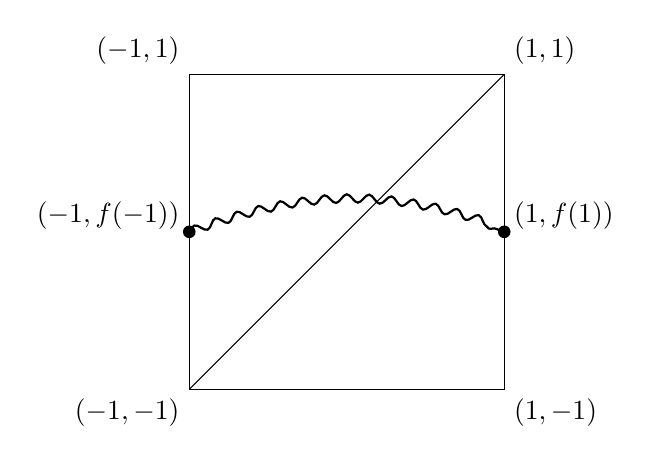
\begin{tikzpicture}[scale=2]

  % Square
  \draw (-1,-1) rectangle (1,1);

  % Diagonal
  \draw (-1,-1) -- (1,1);

  % Corner labels
  \node[above left]  at (-1,1)  {$(-1,1)$};
  \node[above right] at (1,1)   {$(1,1)$};
  \node[below left]  at (-1,-1) {$(-1,-1)$};
  \node[below right] at (1,-1)  {$(1,-1)$};

  % Points a and b
  \fill (-1,0) circle (0.04);
  \fill (1,0)  circle (0.04);

    % Wavy function line between the two points
    \draw[decorate, decoration={snake, amplitude=1.5pt, segment length=8pt}, thick]
        (-1,0) to[out=20,in=160] (1,0);

    \node[left]  at (-1,0.1) {$(-1,f(-1))$};
    \node[right] at (1,0.1) {$(1,f(1))$};

\end{tikzpicture}
    \end{center}

    However, the general case is not easy to prove, and the connectness will be a hard condition to use, the dilemma is that we do not have a good property like intermideate value theorem for any \(n\), in another word, the topology of real line is special.
\end{remark}

\begin{proof}
    Here is a proof by homology theory, which is a pure algebraic topology method, we sketch the outline here:\\
    (1) Assume that there exists a continous function \(f\) without fixed point when \(n\geq 2\), then we can construct a retraction \(r:D^n \to \sph^{n-1}\) by method of analytic geometry.\\
    (2) We claim that there is no retraction from \(D^n\) to \(\sph^{n-1}\) by homology theory, and prove it.\\
    (3) conclude the result.\\

    \textbf{Here are the details:}\\
    (1) For any \(x \in D^n\), we define that \(r(x)\) is the intersection of \(\sph^{n-1}\) and the ray line from \(f(x)\) to \(x\):
      \begin{center}
        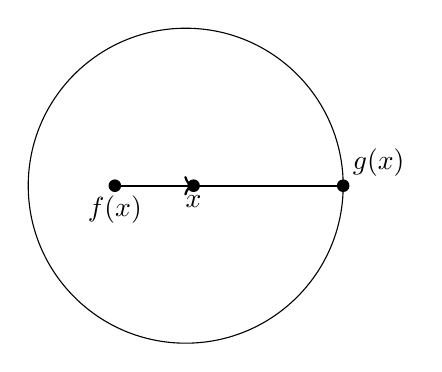
\begin{tikzpicture}[scale=2]

  % Unit ball (circle)
  \draw (0,0) circle (1);

  % Points: f(x), x, g(x) are collinear on the x-axis
  \coordinate (fx) at (-0.45,0);
  \coordinate (x)  at (0.05,0);
  \coordinate (gx) at (1,0);   % on the boundary

  % Draw the line from f(x) through x to g(x)
  \draw[thick] (fx) -- (gx);

  % Arrow from f(x) to x
  \draw[->, thick] (fx) -- (x);

  % Mark points
  \fill (fx) circle (0.04);
  \fill (x)  circle (0.04);
  \fill (gx) circle (0.04);

  % Labels
  \node[below] at (fx) {$f(x)$};
  \node[below] at (x)  {$x$};
  \node[above right] at (gx) {$g(x)$};

\end{tikzpicture}
    \end{center}
    By vector we can write
    \[r(x) = x + \lambda(x-f(x)), \quad \lambda \neq 0 \text{ iff } \|x\|\neq 1\]
    by \(\|r(x)\|=1\), we can get a quadratic equation of \(\lambda\)
    \[\|x-f(x)\|^2 \lambda^2 + 2\langle x, x-f(x) \rangle \lambda + \|x\|^2 - 1 = 0\]
    with the positive determination, we can get the exact formula of \(\lambda\), which is dependent of \(x\) continously
    \[\lambda(x) = \frac{-2\langle x, x-f(x)\rangle+2 \sqrt{\langle x, x-f(x) \rangle^2-\|x-f(x)\|^2(\|x\|^2-1)}}{2\|x-f(x)\|^2}\]
    in particular, when \(x \in \sph^1\) i.e. \(\|x\|=1\), we can get
    \[\lambda(x) = \frac{-\langle x,f(x) \rangle +  \sqrt{\langle x,f(x) \rangle^2}}{\|x-f(x)\|^2} = 0\]
    hence \(r(x) = x\), which means that \(r\) is a retratction from \(D^n\) to \(\sph^{n-1}\).\\

    (2) We prove the claim by homology theory, notice that we have the following commutative diagram:
    
% https://q.uiver.app/#q=WzAsMyxbMSwwLCJEXm4iXSxbMCwxLCJcXG1hdGhiYntTfV57bi0xfSJdLFsyLDEsIlxcbWF0aGJie1N9XntuLTF9Il0sWzEsMCwiaSJdLFswLDIsInIiXSxbMSwyLCJpZCIsMl1d
\[\begin{tikzcd}
	& {D^n} \\
	{\mathbb{S}^{n-1}} && {\mathbb{S}^{n-1}}
	\arrow["r", from=1-2, to=2-3]
	\arrow["i", from=2-1, to=1-2]
	\arrow["id"', from=2-1, to=2-3]
\end{tikzcd}\]
    then by the functoriality of homology, we have the commutative diagram:
    % https://q.uiver.app/#q=WzAsMyxbMSwwLCJIX2soRF5uKSJdLFswLDEsIkhfayhcXG1hdGhiYntTfV57bi0xfSkiXSxbMiwxLCJIX2soXFxtYXRoYmJ7U31ee24tMX0pIl0sWzEsMCwiaV8qIl0sWzAsMiwicl8qIl0sWzEsMiwiaWRfKiIsMl1d
\[\begin{tikzcd}
	& {H_k(D^n)} \\
	{H_k(\mathbb{S}^{n-1})} && {H_k(\mathbb{S}^{n-1})}
	\arrow["{r_*}", from=1-2, to=2-3]
	\arrow["{i_*}", from=2-1, to=1-2]
	\arrow["{id_*}"', from=2-1, to=2-3]
\end{tikzcd}\]
    notice that \(H_{n-1}(D^n) = 0\) and \(H_{n-1}(\sph^{n-1}) \cong \zz\), so \(i_*\) is the trivial map, and \(id_* = r_* \circ i_*\) is also the trival map, which leads to a contradiction (functor keeps idenetity map ).




\end{proof}

There are other proofs by different methods, but generally the fixed point theorem can be generalized to Banach space by the projective theory.

\begin{theorem}[Schauder]
    Let $X$ be a Banach space and let $K \subset X$ be a nonempty, closed, convex set.
If $f : K \to K$ is continuous and compact (i.e.\ $f(K)$ is relatively compact),
then $f$ has a fixed point in $K$.
\end{theorem}

\newpage
\section{Complex Analysis}
\subsection{Holomorphe function}

As a vector space \(\cc\), it is dimension 2 over \(\rr\) but dimension 1 over \(\cc\), although sometimes complex analysis is seen as a special case of real analysis in \(\rr^2\), but the differential structure is quite different.

\begin{lemma}
    Define two vector space as following:
    \[\mathcal{L}_{\cc}(\cc) = \{u: \cc \to \cc \mid \forall x,y \in \cc, \forall c \in \cc, u(x+cy) = u(x) + cu(y)\}\]
    and
    \[\mathcal{L}_{\rr}(\cc) = \{v: \cc \to \cc \mid \forall x,y \in \cc, \forall r \in \rr, v(x+ry) = v(x) + rv(y)\}\]
    where \(\mathcal{L}_{\cc}(\cc)\) is the set of \(\cc\)-linear maps from \(\cc\) to \(\cc\), and \(\mathcal{L}_{\rr}(\cc)\) is the set of \(\rr\)-linear maps from \(\cc\) to \(\cc\). Then\\

    - \(\mathcal{L}_{\rr}(\cc)\) is a vector space over \(\rr\) with dimension \(2\), and a basis is given by
    \[dz: z \mapsto z , \quad d\bar{z}: z \mapsto \bar{z}\]

    - \(\mathcal{L}_{\rr}(\cc)\) has another basis
    \[dx:z \mapsto \Re(z), \quad dy: z \mapsto \Im(z)\]
    and the relation between two basis is given by
    \[dz = dx + i dy, \quad d\bar{z} = dx - i dy\]

    - \(\mathcal{L}_{\cc}(\cc)\) is a vector space over \(\cc\) with dimenson \(1\), and it is the subspace of \(\mathcal{L}_{\rr}(\cc)\) with \(\{dz\}\) as a basis.\\
\end{lemma}
\begin{proof}
    
\end{proof}

A complex function \(f\) can be naturally seen as a real function
\[F: \rr^2 \to \rr^2, \quad (x,y) \mapsto (\Re[f(x+iy)], \Im[ f(x+iy)])\]
Hence we can consider the differentiability of \(F\) in the sense of real function, and its differentiability reflects the property of \(f\) but not equivalent, It is the difference between complex analysis and real analysis.

\begin{definition}
    Let \(U \subset \cc\) be an open set, a function \(f: U \to \cc\) is called \textbf{holomorphe} at \(z_0 \in U\) if there exists a \(\cc\)-linear map \(L \in \mathcal{L}_{\cc}(\cc)\) such that 
    \[f(z_0+h) = f(a) + L(h) + o(|h|)\]
    If \(f\) is holomorphe at any point of \(U\), then we say that \(f\) is holomorphe on \(U\), and we denote the set of all holomorphe functions on \(U\) by \(\mathcal{O}(U)\).
\end{definition}

Equivalently, we also call "holomorphe" by \textbf{"\(\cc\)-differentiable"}, immediately a complex function is called \textbf{"\(\rr\)-differentiable"} if \(L\) is \(\cc\)-linear map in the definition above, but it actually means that the correspondece real function \(F\) is differentiable in the sense of Banach space \(\rr^2\). 

In paticular \(\cc\)-differentialble is \(\rr\)-differentiable, but conversely it is not true. We consdier the example \(f(z) = \bar{z}\)
The coorespondent real function is
\[F: \rr^2 \to \rr^2, \quad (x,y) \mapsto (x,-y)\]
which is clearly \(\rr\)-differentiable at any point with the invertible Jacobian matrix
\[J_F(x,y) = \begin{pmatrix}1 & 0 \\ 0 & -1\end{pmatrix}\]
However, it is not holomorphe (\(\cc\)-differentiable) at any point: Assuming that it is holomorphe at \(z_0\), then there exists a \(\cc\)-linear map \(L\) such that
\[\overline{z_0+h} = \bar{z_0} + L(h) + o(|h|)\]
By the structure of \(\cc\)-linear map, then \(L(h)=ch\) for some \(c \in \cc\), hence
\[\frac{\bar{h}}{h} = c + \frac{o(|h|)}{h}\]
as \(h\) tends to zero, The right side tends to \(c\) while the left side does not have a limit, which is absurd. It is necessary to avoid the confusion between the two type of differentiable case, to get rid of the notation of \(dx\) and \(dy\), sometimes it is terrible.

If \(f:U \to \cc\) is \(\rr\)-differentiable, in the sense of real function, its differentible at \(a \in U\), as a \(\rr\)-linear map, can be written as
\[(D_f)_a = \frac{\partial f}{\partial x}(a) dx + \frac{\partial f}{\partial y}(a) dy\]
with two \(\rr\)-linear maps \(dx\) and \(dy\), then we can change the basis \(\{dx, dy\}\) to \(\{dz, d\bar{z}\}\):
\[(D_f)_a = \frac{\partial f}{\partial z}(a) dz + \frac{\partial f}{\partial \bar{z}}(a) d\bar{z}\]

\begin{definition}
    The \textbf{Wirtinger operators} are defined by
    \[\frac{\partial}{\partial z} = \frac{1}{2}\left(\frac{\partial}{\partial x} - i \frac{\partial}{\partial y}\right), \quad \frac{\partial}{\partial \bar{z}} = \frac{1}{2}\left(\frac{\partial}{\partial x} + i \frac{\partial}{\partial y}\right)\]
\end{definition}

Hence under the differetial operator with respect to \(z\) and \(\bar{z}\), the complex function \(f\) can be independent of \(x\) and \(y\) completely, with the following properties of differential:

\begin{enumerate}
    \item For any \(\rr\)-differentiable function \(f:U \to \cc\)
    \[\overline{\frac{\partial f}{\partial z}} = \frac{\partial \bar{f}}{\partial \bar{z}}\]
    \item For any \(\rr\)-differentiable function \(f,g:U \to \cc\),
    \[\frac{\partial (fg)}{\partial z} = f \frac{\partial g}{\partial z} + g \frac{\partial f}{\partial z} \quad \frac{\partial (fg)}{\partial \bar{z}} = f \frac{\partial g}{\partial \bar{z}} + g \frac{\partial f}{\partial \bar{z}}\]
    \item For any \(\rr\)-differentiable \(f:U \to \cc\) and \(g: f(U) \subset V \to \cc\)
    \[\frac{\partial (h \circ g)}{\partial z} = (\frac{\partial h}{\partial w}\circ g) \cdot \frac{\partial g}{\partial z} + (\frac{\partial h}{\partial \bar{w}}\circ g) \cdot \frac{\partial \bar{g}}{\partial z}\]
    and 
    \[\frac{\partial (h \circ g)}{\partial \bar{z}} = (\frac{\partial h}{\partial w}\circ g) \cdot \frac{\partial g}{\partial \bar{z}} + (\frac{\partial h}{\partial \bar{w}}\circ g) \cdot \frac{\partial \bar{g}}{\partial \bar{z}}\]

\end{enumerate}

Although the holomorphe function is different from real differntiable function, but we can not omit the realtion between them, and in many cases the correspondent real function is easier to study, hence the following proposition is important:
\begin{proposition}
    If \(U \subset \cc\) is open and \(f:U \to \cc\) is a complex function, then the following conditions are equivalent:\\
    (1) \(f\) is holomorphe on \(U\).\\

    (2) \(f\) is \(\rr\)-differentiable on \(U\) and \(\frac{\partial f}{\partial \bar{z}} = 0\) on \(U\).\\

    (3) Writing \(f = u + iv\) with real functions \(u,v:U \to \rr\), then \(u\) and \(v\) are \(\rr\)-differentiable on \(U\) and satisfy the \textbf{Cauchy-Riemann equations}:
    \[\frac{\partial u}{\partial x} = \frac{\partial v}{\partial y}, \quad \frac{\partial u}{\partial y} = -\frac{\partial v}{\partial x}\]

    In particular, if \(f\) is holomorphe at \(a = p+iq \in U\), then its \(\cc\)-derivative at \(a\) is given by
    \[f'(a) = \frac{\partial f}{\partial z}(a) = \frac{\partial f}{\partial x}(a) = 2 \frac{\partial u}{\partial z}(a)\]
    and write \(F\) as the correspondent real function of \(f\), the Jacboian of \(F\) at \((p,q)\) is
    \[\det J_F(p,q) = |f'(a)|^2\]
\end{proposition}
\begin{proof}
    
\end{proof}

In the sense of complex analysis, the constant function are a very strong condition by comparison with real analysis, hence local constant condition can imply global constant condition in some requirement of connectness.
\begin{corollaryplain}
    Let \(D \subset \cc\) be a connected open set, then the following conditions are equivalent:\\
    (1) \(f\) is constant. \qquad (2) \(f' = 0\).\qquad  (3) \(|f|\) is constant.\\
    (4) \(\Re(f)\) is constant. \qquad (5) \(\Im(f)\) is constant. 
\end{corollaryplain}

\subsection{Cauchy's Integral Formula}

By the view of manifold, \(\cc\) can be seen as a \textbf{2-dimensional real manifold} with a complex structure, hence it is natural to consider the differential form on it. Let \(f: U \to \cc\) a differenetiable function on an open set \(U \subset \cc\), then it induces a differential
\[df: U \to \mathcal{L}_{\rr}(\cc), \quad a \mapsto (Df)_a = = \frac{\partial f}{\partial z}(a) dz + \frac{\partial f}{\partial \bar{z}}(a) d\bar{z}\]

about the \(d(df) = ...\)

\begin{definitionplain}
    Let \(U\) be an open set in \(\cc\), and then we define 
    \begin{align*}
        \text{0-form}: & \quad \Omega^0(U) = C^{\infty}(U,\cc) \\
        \text{1-form}: & \quad \Omega^1(U) = \{f dz + g d\bar{z} \mid f,g \in C^{\infty}(U,\cc)\}\\
        \text{2-form}: & \quad \Omega^2(U) = \{h d\bar{z} \wedge dz \mid h \in C^{\infty}(U,\cc)\}
    \end{align*}
    and generally we define differential forms on \(U\) by
    \[\Omega(U) = \bigoplus_{k=0}^2 \Omega^k(U)\]
\end{definitionplain}




As the one of the most part in complex analysis, cauchy's integral formula shows the deep relation between the integral and holomorphe function, in this section we will give a general statement with the help of differential form, and we will see that it is a application of stoke's theorem in complex plane, i.e. Green-Riemann theorem.

\begin{theorem}[Green-Riemann] $ \\$
    Let \(K\) be a compact with smooth boundary \(\partial K\) in \(\cc\), and \(w \in \Omega^1(\mathring{K})\) be a 1-form of class \(C^1\), then
    \[\int_{K} dw = \int_{\partial K}w\] 
\end{theorem}

\begin{proof}
    
\end{proof}

The classic statement of Cauchy's integral formula is that if \(f\) is holomorphe on an open set \(U\), then for any point \(a \in U\) and a open ball \(B(a,r) \subsetneq U\), then
\[\int_{C(a,r)}fdz  = 0\]
where \(C(a,r)\) is the circle cnetre at \(a\) with radius \(r\) and positive orientation, it can be seen as the boundary of the \(B(a,r)\), and \(fdz\) is always a closed 1-form of class \(C^1\), hence by Greee-Riemann formula, the formula holds. But we can do more with the Green-Riemann theorem, it gives a more general statement about the reigion of integration.

\begin{theorem}[1912, Cauchy-Pompeiu] $ \\$
    Let \(U\) be an open subset of \(\cc\) and \(K\) is a compact of \(U\) with smooth boundary \(\partial K\), if \(f \in C^1(U)\), then we have
    \[\frac{1}{2\pi i}\int_{\partial K} \frac{f(z)}{z - a} dz + \int_{K} \frac{\partial f}{\partial \bar{z}}(z) \frac{1}{z - a} d\bar{z} \wedge dz = \begin{cases}
        f(a) & a \in \mathring{K} \\ 0 & a \in \cc-K
    \end{cases}\]
    in particular, if \(f \in \mathcal{O}(U)\) holomorphe,
    \[\int_{\partial K} fdz = 0\]
    and for any \(a \in \mathring{K}\),
    \[f^{(k)}(a) = \frac{k!}{2\pi i }\int_{\partial K} \frac{f(z)}{(z - a)^{k+1}} dz\]
\end{theorem}




\subsection{Analytic function}


previous section, it is an important properties, it claims that the local value of the power series determines the global vaule. In general, two analytic function \(f\) and \(g\), if they are equal in a local voinsinage \(V\), then for any \(x \in V\), there exists a open ball \(B(x,r)\) such that their power series expanasions are equal. The most important things is that \(V\) is not compact, so our open cover \(B(x,r)\) will bring the properties by extending, so \(f\) and \(g\) are actually equal!

The statement above is a little abstract, it is better to draw a picture from a voinsinage \(V\), then see that if we want to let \(f=g\) we just need to consider the point nearly the \(\partial V\)... 

In this section we will prove the analytic continuation, and three other important theorems in complex anaylsis, although they have various methods to porve, but here our inspiration is continuation:
\[\text{Analytic continuation} \implies \text{Isolated zero} \implies \text{Open mapping} \implies \text{Maximum modulus}\]

\begin{theorem}[analytic continuation]$ \\$
    Given an \textbf{open and connect} set \(U\) in complex plane, and \(f,g: U \to \cc\) are two holomorphic (analytic) functions. If they are equal in a voinsinage of \(U\), then \(f=g\) in whole \(U\).

    \begin{proof}
        We let \(S = \{z \in U |f^{(n)}(z) = g^{(n)}(z) \text{ for any} n \in \nn \}\), and clearly \(S = \bigcup_{n \in \nn}\{z\in U| f^{(n)}(z) = g^{(n)}(z)\}\). It is easy to verify that \(S\) is the intersection of infinite closed sets, so \(S\) is closed.

        \(S\) is also open. We take any \(z_0 \in S\), we notice that \(S\) is a subset of the voinsinage where \(f\) and \(g\) are equal, then by corollary \ref{analytic continuity series}, it implies that they have the same seires in a voinsinage of \(z_0\) contained in \(S\), then clearly \(f^{(n)}(z) = a_n = b_n = g^{(n)}(z)\) in the voinsinage, so that \(S\) must be open. What's more \(S\) is not empty, and \(U\) is connect, so \(U=S\).

    \end{proof}
\end{theorem}

\begin{remark}
        We notice that the proof is based on the topological property of the domain \(U\), so the properties of holomorphic is speacial.
\end{remark}

    One directly result of analytic continuation is the isolated zero theorem, it claims that the zero of a holomorphic function must be discrete:

\begin{theorem}[isolated zero]
        Suppose that \(U\) is \textbf{an open and connect set} in complex plane, and \(f \in H(U)\) is a non-zero holomorphic function, then\\
        - If \(z \in U\) such that \(f(z_0) = 0\), then \(f\) can be expended in a neighborhood \(\Omega \subset U\):
        \[f(z) = (z-z_0)^ng(z)\]
        where \(g\) is a non-vanishing holomorphic function in \(\Omega\). \\
        - Any zero \(z_0\) of \(f\), there exists a neighborhood such that \(z_0\) is the unique zero in the neighborhood. \\
        - The set of all zeros of \(f\) is discrete.

    \begin{proof}
            If \(z_0\) is a zero, then there exists a expanasion of power series near the \(z_0\) with 
            \[f(z) = \sum_{k \in \nn}a_k(z-z_0)^k, \quad a_0 =0\]
            So we just take \(n = \min\{i \in \nn| a_i \neq 0\}\), then 
            \[f(z) = (z-z_0)^n\sum_{k \in \nn}a_{n+k}z^k\]
            So we just take \(g(z) = \sum_{k \in \nn}a_{n+k}z^k\). It is well-defined since in a small reigon near \(z_0\) and does not contain \(z_0\) we have surely \(g(z) = \frac{f(z)}{(z-z_0)^n}\), then by analytic continuation \(g\) is holomorphic on a samll neighborhood with \(z_0\) in it, and \(g(z_0) = a_n \neq 0\). Hence by continuity, there exists a positive \(r>0\) such that 
            \[||f(z_0)|-|a_n|| \leq |f(z_0)-a_n| < |a_n| /2\]
            for any \(z \in B(z_0,r)\), which implies \(|f(z_0)| > |a_n|/2 > 0\) in the reigon, so it is non-vanishing. Just take the intersection of the previous neighborhood and \(B(z_0,r)\), then we get the \(\Omega\) we hope.

            The second statement is immediate from the first statement. For the third, if there exists a limit point \(a\) in the set of zeros, then for any small neighborhood with \(a\) in it, it will conatins infinite other zeros, which contradicts with the second statement.
    \end{proof}
\end{theorem}

    With the help of the isolated zero theorem, we can generalize the analytic continuation, locally two holomorphic function are just equal in a non-discrete set:

    \begin{theorem}[strong analytic continuation]
        Given an \textbf{open and connect} set \(U\) in complex plane, and \(f,g: U \to \cc\) are two holomorphic (analytic) functions. If they are equal in a set \(S \subset U\), and \(U\) admet an accumulation point, then \(f=g\) in \(U\).

        \begin{proof}
            Just take \(f-g\) as the new holomorphic function in U, notice it will be zero in \(S\) and \(S\) is not discrete, so \(f-g\) must be zero by isolated zero.
        \end{proof}
    \end{theorem}

    \begin{remark}
        An direct result if two holomorphic functions are equal in a non-constant convergent sequence, then they will behave equal globally.
    \end{remark}

    The other two result is the maximum modulus principle and open mapping theorem.

    \begin{theorem}[open mapping]$ \\$
        A non-constant holomorphic function defined on \textbf{an open and connect set }must be an open map.

        \begin{proof}
            Take any \(z_0 \in U\), and we will prove that \(f(z_0) \in f(U)\) must be an interior point. By isolated zero theorem, there exists \(B=B(z_0,r) \subset U\) such that in it we have
            \[f(z) - f(z_0) = (z-z_0)^ng(z)\]
            so \(f\) can be written as the composition of the following holomorphic functions:\\
            - \(u:z \mapsto (z-z_0)g^{1/n}(z)\) from \(B\) to \(\cc\).\\
            - \(v:z \mapsto z^n\) from \(\cc\) to \(\cc\).\\
            - \(t:z \mapsto z+f(z_0)\) from \(\cc\) to \(\cc\).\\
            so \(f = t \circ v \circ u\), we just need to verify the three maps are open, it can be proved via \textbf{the local inversion theorem: if the derivative is not zero at some point, then locally there exists a diffeomorphism, so the image of the point will be an interior.}

            For \(u\) we can compute \(u'(z) = g^{1/n}(z) + \frac{(z-z_0)}{n}g'(z)g^{\frac{1-n}{n}}(z)\), clearly \(u'(z_0) =g^{1/n}(z_0) \neq 0\), and \(u\) is holomorphic so class of \(C^1\), so locally there exists a diffeomorphism between neighborhoods \(U_{z_0}\) and \(V_{u(z_0)}\), so \(u(z_0)\) is a interior point of \(f(B)\).

            For \(v\) the proof is similar if we take \(z_0 \neq 0\) since \(v'(z) = nz^{n-1}\). In the case of \(z_0=0\), we take a enough samll positive \(r>0\), then \(|z| <r\) implies \(|z|^n<r^n\), so \(B(v(0),r) \subset B(0,r^n) = v(B(0,r))\), so \(v\) is open. Finally, \(t\) is clearly open. Thus after composition, \(f\) is open.
        \end{proof}
    \end{theorem}

\begin{theorem}[Maximum modulus]$ \\$
    If \(f\) in a non-constant holomorphic function on \textbf{an open and connect set} \(U\), then \(|f|\) can not attain a maximum in \(U\).\\
    -Weakly, if \(K \subset U\) is a compact set, then \(|f|_K|\) attain the maximum in the boundary:
    \[\sup_{z \in K}|f(z)| \leq \sup_{\partial K}|f(z)|\]

    \begin{proof}
        Assume that \(f\) did attain a maximum in \(z_0 \in U\), then we take a small voinsinage of \(x_0\), called \(V\), by open mapping theorem \(f(V)\) must be open with \(f(z_0)\) in it, so there exists \(r>0\) such that \(B(f(z_0),r) \subset f(D)\). We take \(\delta = sign(Re(f(z_0)))\), then \(f(z_0) + \delta\frac{r}{2} \in f(D)\), we denote it \(f(w_0)\), then \(|f(w_0)| > |f(z_0)|\) clearly, which contradicts with the assumption.

        The weakly statement is immediate since \(|f|\) is continous, so \(f(K)\) will be compact in \(\rr\), so \(|f|\) must attain a maximum in \(K\), with the strong statement we know that the maximum can not be in \(int(K)\), so in boundary.
    \end{proof}
\end{theorem}






\subsection{Infinite Product}
The form of infinite products is important in complex analysis to study the poles and zeros of functions, here is the definition:

\begin{definition}
    Let \((a_n)_{n=1}^{\infty}\) be a sequence of complex numbers. The infinite product \(\prod_{n=1}^{\infty} a_n\) is said to converge if there exists \(N \in \nn\) such that:\\
    (1) \(a_n \neq 0\) for all \(n \geq N\)\\
    (2) the sequence of partial products\((\prod_{k=n}^N a_k)_{n \geq N}\) converges to a non-zero limit as \(n \to \infty\).\\
If the limit is zero, we say the product \textbf{diverges to zero}. If the limit does not exist, we say the product diverges.
\end{definition}
we avoid the case that some terms are zero, because it will make the product zero, which is not interesting; and we notice that if the sequence \((a_n)\) converges to zero, then the product will tend to zero trivally, so we need to avoid this case too. Anyway, the definition here is delicated enough to avoid any trival case.

\begin{proposition}[The properties of convergence]
    Let \((a_n)_{n=1}^{\infty}\) be a sequence of complex numbers such that the infinite product \(\prod_{n=1}^{\infty} a_n\) converges, then:\\
    (1) \(\lim_{n \to \infty} a_n = 1\)\\
    (2-LOG) If \(a_n \in \cc-\rr_{-}\) for sufficent large \(n\), then we have equivalent conidtion for the convergence of the product: the series \(\sum_{n=1}^{\infty} \Log a_n\) converges.\\
    (3-CVA) If \(\sum_{n \in \nn} |a_n| < \infty\), then the product \(\prod_{n=1}^{\infty} 1+a_n\) converges or diverges to zero.

    \begin{proof}
        (1) is immediate form \(a_n = (\prod_{k=1}^{n}a_k/\prod_{k=1}^{n-1}a_k)\) for \(n \geq 2\).\\
        (2) By the convergence of (1), for sufficent large \(n\), \(a_n\) stays near 1, hence we can choose the principal branch such that for sufficent large \(N\)
        \[\Log \prod_{n \geq N}a_n = \sum_{n \geq N} \Log a_n\]
        (3) If \(\sum_{n \in \nn} |a_n| < \infty\), so \(a_n\) converges to zero so we can expend 
        \begin{align*}
            \Log(1+a_n) = a_n-\frac{a_n^2}{2} + o(a_n^3)
        \end{align*}
        Then by (2), the series \(\sum_{n \in \nn} \Log(1+a_n)\) converges absolutely, hence the product converges or diverges to zero.
        
    \end{proof}
\end{proposition}

With the basic technics, we can study the products of fuctions, that's the core to construct some important functions like gamma function.
\begin{definitionplain}[Convergence of product of functions] $ \\$
    Let \((f_n)_{n \in \nn}\) be a sequence of continous function on a open set \(U\)\\
    - The product \(\prod_{n \in \nn} f_n\) converges pointwise to \(F\) on \(U\) if for each \(z \in U\), the product \(\prod_{n \in \nn} f_n(z)\) converges to \(F(z)\).\\
    - The product \(\prod_{n \in \nn} f_n\) converges uniformly to \(F\) on \(U\) if there exists \(N \in \nn\) such that for all \(n \geq N\), \(f_n\) does not vanish on \(U\) and the sequence of partial products \((\prod_{k=n}^N f_k)_{n \geq N}\) converges uniformly to \(F\) on \(U\).
\end{definitionplain}
Here is the definition following above definition, the zero of the functions in sequence may cause some problems, so there are some difficult in definition. Another clear definition is from \textbf{Henri Cartan's book}, here we give as a lemma:

\begin{lemma}
    In above definition, let \(K \subset U\) as a subset, then the product \(\prod_{n \in \nn} f_n\) converges uniformly on \(K\) if \(f_n\) satisfies the following condition:\\
    (1) \((f_n)_{n \in \nn}\) coverges uniformly to \(1\) on \(K\).\\
    (2) The series \(\sum_{n \in \nn}\Log f_n\) converges normally on \(K\).

    \begin{proof}
        By (1), for sufficent large \(N\), we have \(|f_N - 1| < 1/2\), so for all \(n \geq N\), \(\Log f_n\) is well defined and  \(f_n\) does not vanish on \(K\). so for any \(z \in K\)
        \[\Log \prod_{k=n}^N |f_k| = \sum_{k=n}^N |\Log f_k| \leq \sum_{k=n}^N \|\Log f_k\|_{K}\]
        it implies that the sequence of partial products converges uniformlly on \(K\) by weierstrass M-test. 
    \end{proof}
\end{lemma}

Infinite products is a strong tool to construct function with certain zeros, for example we can constryct a function with zeros at all integers like following:
\[z \prod_{n \geq 1} (1 - \frac{z^2}{n^2})\]
It is not difficult to verify that he product converges locally uniformlly to a holomorphic function, and one holomorphic function sharing the propoerties is \textbf{sine function}, actually we can prove that they are equally up to a constant factor, which is a famous result called \textbf{Euler's sine product formula}. With the following proposition, we can completely prove the formula:
\[\sin(\pi z) = \pi z \prod_{n \geq 1} (1 - \frac{z^2}{n^2})\]
The proof can be found in [Stein 2, page 142].
\begin{proposition}
    Let \((f_n)_{n \in \nn}\) be a sequence of holomorphic functions on an open set \(\Omega \subset \cc\), and suppose that the product \(\prod_{n \in \nn} f_n\) converges  \(\Omega\) to a function \(f\) locally uniformly, then\\
    (1) \(f\) is holomorphic on \(\Omega\)\\
    (2) The zeros and multiplicities of \(f\) follows from the sequence:
    \[Z(f) = \bigcup_{n \in \nn} Z(f_n) \qquad m_f(z)= \sum_{n \in \nn} m_{f_n}(z)\] 
    (3) If \(f_n\) does not vanish on \(\Omega\) for any \(n\), then the series of meromorphic functions \(\sum_{n \in \nn} f_n'/f_n\) converges locally uniformly on \(\Omega - Z(f)\) to \(f'/f\).
\end{proposition}
\begin{proof}
    It's the result of locally uniformlly convergence on the inifinite product, notice that the proof of (3) is referred to a idenetity:
    \[\frac{(\prod_{k=1}^nf_k)'}{\prod_{k=1}^nf_k} = \sum_{k=1}^n \frac{f_k'}{f_k}\]
    which can be proved by induction. Another point is that the proof of (2) needs that the multiplicities of zeros are finite, i.e. for any \(a \in \Omega\) we have
    \[\#\{n\in \nn | f_n(a) = 0\} < \infty\]
    Which is ensured by the definition of convergence of infinite product.
\end{proof}

There are two natural question arsing from Euler's formula, one is that if we find another entire function with zeros at all integers, whether the function is same with sine function up to coefficients or anything else? The other is that if there exists a general method to construct entire function with given finite or infinite zeros? The answer is from \textbf{Weierstrass's} construction.

Firstly, the zeros of holomorphic is isolated or discrete, so we the given zeros can not have any limit point in \(\cc\), hence the problem is limited to discrete set of points. \textbf{For finite zeros, we can use the fundamental theorem of algebra to construct a polynomial with given zeros}, so the problem is limited to infinite zeros. By Borel-Weierstrass theorem, we can deuduce that the set of zeros must be unbounded.

Another point about zero is that the multiplicity of zeros must be finite. Suppose that \(f\) is an non-zero entire function, then by propoerty of analytic function, \(f\) can be expended at any point \(z_0\) as a Taylor series
\[f(z) = \sum_{n=0}^{\infty} \frac{f^{(n)}(z_0)}{n!} (z - z_0)^n\]
If \(z_0 \) is a zero with inifinite multiplicity, then \(f^{(n)}(z_0) = 0\) for all \(n \in \nn\), hence \(f \equiv 0\) in the neighborhood of \(z_0\), which implies \(f \equiv 0\) in \(\cc\) by analytic countiuation, it is absurd. Together with the above statement, if \((a_n)_{n \in \nn}\) is the sequence of zeros, then the zeros must satisfy \(\lim_{n \to \infty} |a_n| = \infty\).

With the basic analysis of zeros, now we can consrtuct the entire function by given zeros. Notice that we can not simply combine the zeros together by linear terms
\[\prod_{n \in \nn} (z-a_n)\]
The product diverges for infinite unbounded zeros, so we can copy the idea of Euler's formula, i.e.
\[\prod_{n \in \nn} (1 - \frac{z}{a_n})\]
However, we can not ensure the convergence of the product, for example we take zeros as all positive integers. To ensure the convergence we need to add some extra terms in each factor, that is called \textbf{Weierstrass's canonical factors}.

\begin{lemma}
    We define the weierstrass's canonical factor of the degree \(p\) as
    \[E_p(z) := \begin{cases}
        (1-z) & p=0 \\
        (1-z)e^{(z + \frac{z^2}{2} + \cdots + \frac{z^p}{p})} & p \in \nn
    \end{cases}\]
    then the factor has the following propoerties:\\
    (1) It is an entire function with a simple zero at \(z=1\) and no other zeros.\\
    (2) It is a function of finite order \(p+1\).\\
    (3) For \(|z| \leq r <1\), we have the estimate
    \[|E_p(z)-1| \leq C_r|z|^{p+1}\]
    for some constant \(C_r > 0\). That means the larger the \(p\) is, the convergence of \(E_p(z)\) to 1 is faster.
\end{lemma}
\begin{proof}
    (1) and (2) is clear, we prove (3).
    \begin{align*}
        \log(E_p(z)) &= \log(1-z) + z + \frac{z^2}{2} + \cdots + \frac{z^p}{p}  \\
        &= -\sum_{n=1}^{\infty} \frac{z^n}{n} + (z + \frac{z^2}{2} + \cdots + \frac{z^p}{p}) \\
        &= -\sum_{n=p+1}^{\infty} \frac{z^n}{n} = O(|z|^{p+1})
    \end{align*}
    the expansion here is ensured by \(|z| < 1\), hence
    \[E_p(z) = \exp(\log E_p(z)) = 1 + O(|z|^{p+1})\]
    by expansion of expoential function \(e^z = 1+z+o(z^2)\), so we can conlude the result.
\end{proof}

So we can response the original question by collecting the above ideas:
\begin{theorem}[Weierstrass's Factorization Theorem] $ \\$
    Let \((a_n)_{n \in \nn}\) be a sequence of complex numbers such that \(\lim_{n \to \infty} |a_n| = \infty\), and we make convention that \(E_n(\frac{z}{0}):= z\), then the infinite product
    \[f(z) = \prod_{n=1}^{\infty} E_{n}(\frac{z}{a_n})\]
    converges locally uniformly in \(\cc\) to an entire function \(f\) whose zeros are precisely the points \(a_n\), with multiplicities by counting. Moreover, if \(g\) is any other entire function with the same zeros and multiplicities, then there exists an entire function \(h\) such that
    \[g(z) = f(z)e^{h(z)}\]
    for all \(z \in \cc\).
    
\end{theorem}

Another better theorem is given by \textbf{Hadamard}, it shows the growth of the entire function will influence the construction of the function by given zeros.
\begin{theorem}[Hadamard's Factorization Theorem] $ \\$
Suppose that \(f\) is an entire function of finite order \(\rho\) with zeros \((a_n)_{n \in \nn}\) (counting multiplicities), then there exists a polynomial \(P\) of degree at most \(k=\lfloor \rho \rfloor\) such that
\[f(z) = e^{P(z)}\prod_{n=1}^{\infty} E_{n}(\frac{z}{a_n})\]
\end{theorem}

\subsection{Mellin transformation for analytic continuation}
The Mellin transformation is a integral transformation which is useful in complex analysis to study the analytic continuation of functions. For example,
the gamma function is well-defined for \(\Re(s) > 0\) by the integral
\[\Gamma(s) = \int_0^{\infty} e^{-t}t^{s-1} dt\]
Moreover, zeta function is well-defined for \(\Re(s) > 1\) by the integral \textbf{(Ex15, Chapter6, Stein 2, a easy exercise)}
\[\zeta(s) = \frac{1}{\Gamma(s)}\int_0^{\infty} \frac{t^{s-1}}{e^t - 1} dt\]
and similarly Beta function, a function has a deep relationship with Gamma function, is well-defined for \(\Re(a), \Re(b) > 0\) by the integral \textbf{(Ex7, chapter 6, Stein 2)}
\[B(a,b) = \int_0^{\infty} \frac{t^{a-1}}{(1+t)^{a+b}}  dt\]
Hence we can pay attention to the form of the integration, and then we can a form of integral transformation:
\[\int_0^{\infty}f(t)t^{z-1}dt\]
which is called \textbf{Mellin transformation} of the function \(f\), and we usually denote it by \(\mathcal{M}[f;z]\).


\subsection{Gamma function}

As we have mentioned above, the gamma function is defined by two equivalent forms, this section is to study the specific properties of gamma function.
\begin{definition}
    Let \(\gamma\) be the Euler constant, \(z \in \cc-\zz_{-}\)\\

    -infinite product definition: 
    \[\Gamma(z) = \frac{1}{ze^{\gamma z} \prod_{n \geq 1}(1+\frac{z}{n})e^{-z/n}}\]

    -integral definition:
    \[\Gamma(z) = \int_0^{\infty} t^{z-1}e^{-t} dt\]
    as the mellin transformation of \(f(t) = e^{-t}\).
\end{definition}

The Gamma function is a \textbf{meromorphic} function on \(\cc\) with poles at all \(\zz_{-} =\{0,-1,-2,\dots\} \), and its residues are
\[\mathrm{Res}(\Gamma,-n) = \frac{(-1)^n}{n!}, \quad -n \in \zz_{-}\]
The existence of poles is clear by the infinite product, but the calculation of residues is not clear, it depends on the functional equation to give a simple proof.

\begin{proposition}
    For any \(z \in \cc - \zz_{-}\)
    \[\Gamma(z+1) = z\Gamma(z)\]
    In particular, for any \(n \in \nn\), \(\Gamma(n+1) = n!\).
\end{proposition}

\begin{proof}
    
\end{proof}

\begin{remark}
    With the formula, we can verify the residues at poles easily. For any \(-n \in \zz_{-}\) and \(\Re(z) >-n-1\)
    \[\Gamma(z)(z+n) = \frac{\Gamma(z+n+1)}{z(z+1)\cdots(z+n-1)}\]
    by the functional equation, hence calculate the limit of right term at \(-n\), we can get the residue at \(-n\).
\end{remark}


Guass integration is one of the most famous integration 
\[I = \int_{0}^{\infty}e^{-x^2} dx \]
we can set \(x^2=t\), then subsitute 
\[I = \frac{1}{2} \int_{0}^{\infty} t^{-1/2}e^{-t} dt = \frac{\Gamma(1/2)}{2} \]
hence the gamma function can give the integration result, which motivates the following functional equation:
\begin{proposition}
    For any \(z \in \cc - \zz_{-}\)
    \[\Gamma(z)\Gamma(1-z) = \frac{\pi}{\sin(\pi z)}\]
    In particular, \(\Gamma(1/2) = \sqrt{\pi}\).
\end{proposition}
\begin{proof}
    
\end{proof}
\begin{proposition}[Legendre's Formula]
    For any \(z \notin \zz_{-1}\cap(\zz_{-1}-\frac{1}{2})\)
    \[\Gamma(z)\Gamma(z+\frac{1}{2}) = 2^{1-2z}\sqrt{\pi}\Gamma(2z)\]
    In particular for any \(n \in \nn\)
    \[\Gamma(n+\frac{1}{2}) = \frac{(2n)!}{4^n n!}\sqrt{\pi}\]
\end{proposition}
\begin{proof}
    
\end{proof}

In many case, we need to study the asymptotic behavior of gamma function when \(z \rightarrow \infty\), and gamma function has a deep relation with factoria, a useful equivalent formula help us to do that:
\begin{proposition}[Euler-Gauss's Formula]
    For any \(z \in \cc - \zz_{-}\)
    \[\Gamma(z) = \lim_{n \to \infty} \frac{n! n^z}{z(z+1)(z+2)\cdots(z+n)}\]
    In particular, we have the asymptotic formula:
    \[\Gamma(z+n+1) \sim_{n \rightarrow \infty} n!n^z\]
\end{proposition}

\subsection{Harmonic function}

For the function of class \(C^2\), the laplace operator is defined as
\[\Delta = \frac{\partial^2}{\partial x^2} + \frac{\partial^2}{\partial y^2}\]
By the Wirtinger operators, we can rewrite the laplace opeator as
\[\Delta = 4\frac{\partial^2}{\partial z \partial \overline{z}} = 4\frac{\partial^2}{\partial \overline{z} \partial z}\]

\begin{definition}
    Let \(U \subset \cc\) be an open set and \(K= \cc\) or \(\rr\), a function \(u: U \to K\) of class \(C^2\) is called \textbf{harmonic} if it satisfies the laplace equation:
    \[\Delta u = 0\]
    The set of complex harmonic funnction on \(U\) is denoted by \(\mathcal{H}(U,\cc)\), the set of real hamonic function on \(U\) is denoted by \(\mathcal{H}(U,\rr)\).
\end{definition}

The holomorphe function is naturally related to harmonic function in two senses:
\begin{enumerate}
    \item If \(f \) is holomorphe sur \(U\), then \(\frac{\partial f}{ \partial \bar{z}} = 0\) imples that \(\Delta = 0\).
    \item write \(f\) as \(f = u + iv\), then cauchy Riemann equation gives that
    \[u_x = v_y, \quad u_y = -v_x\]
    holomorphe ensures that \(u\) and \(v\) are of class \(C^{\infty}\) as real-differentiable functions, hence we can apply the lemma of schwartz
    \[\Delta = u_{xx}+u_{yy} = v_{xy} + (-v_{yx}) = 0\]
    and similarly \(\Delta v = 0\), hence \textbf{both real part and imaginary part of holomorphe function are harmonic functions}.
\end{enumerate}

We can see that holomorphe function is a strong condition for harmonic function.

\begin{propositionplain}
    Let \(U \subset \cc\) be an open set and \(f \in \mathcal{O}(U)\), if \(f(z) \neq 0\) for any \(z \in U\), then \(\ln|f| \in \mathcal{H}(U,\rr)\).
\end{propositionplain}

\begin{proof}
    
\end{proof}

A classic question is to find the holomorphe function by a known real part or imaginary part, it refers to the solution of Cauchy-Riemann equation, formally
\begin{definitionplain}
    Let \(u,v: U \to \rr\) be two function of class \(C^2\), then \((u,v)\) is called \textbf{a pari of harmonic conjuagets} on \(U\) if they are all harmonic functions and satisfy the Cauchy-Riemann equation.
\end{definitionplain}

Harmonic conjuagtes allows us to denote a harmonic function as the real (imaginary) part of a holomorphe function.

\begin{proposition}
    Let \(U \subset \cc\) be an open set and \(u: U \to \rr\) be a real harmonic function, then for any \(a\in U\) there exists a neighborhood \(V \subset U\) of \(a\) and a holomorphe function \(f \in \mathcal{O}(V)\) such that
    \[u = \Re(f) \text{ on } V\]
    and locally on \(V\), \(\Im(f)\) is a harmonic conjugate of \(u\).
\end{proposition}



The global existence does not hold in general, for example, we take \(u(z) = \ln|z|\) on \(U = \cc - \{0\}\)

\begin{proposition}[Simply-connectness]$ \\$
    Let \(U \subset \cc\) be a simply-connected open set and \(u: U \to \rr\) be a real harmonic function, then there exists a holomorphe function \(f \in \mathcal{O}(U)\) such that
    \[u = \Re(f) \text{ on } U\]
    generally, \(f \mapsto \Re(f)\) induces an isomrphism between function spaces:
    \[\mathcal{O}(U)/i\rr \xrightarrow{\sim} \mathcal H(U,\rr)\]
\end{proposition}


\begin{proposition}[Mean value property]$ \\$
    Let \(u:U \to \cc\) be a haromonic function on an open set \(U \subset \cc\), then for any \(a \in U\) with \(B(a,r) \subset U\) for some positive \(r>0\), we have
    \[u(a) = \frac{1}{2\pi r}\int_{C(a,r)} u(z) \, |dz| = \frac{1}{2 \pi} \int_{0}^{2\pi} u(a + re^{i\theta}) \, d \theta\]
    where \(C(a,r) = \{z \in \cc | |z-a| = r\}\) is the circle centered at \(a\) with radius \(r\), and \(|dz|\) is the length element on the circle.
\end{proposition}

\begin{proof}
    
\end{proof}

Mean value property shows that the value at a point is determined by the integration along a circle centered at the point, exactly the harmonic function is characterized by this property, that means given the information of the function along the boundary of a disk, we can get all the vaules inside the disk.

\begin{theorem}[Dirichlet problem on \(\mathbb{D}\)] $ \\$
    For any continous function \(\varphi: \mathbb{T} \to \cc\), then there exists a unique continous function \(u: \overline{\dd} \to \cc\) such that \(u\) is harmonic on \(\dd\) and \(u|_{\mathbb{T}} = \varphi\).
\end{theorem}

\begin{proof}
    
\end{proof}

\begin{corollary}
    Let \(f: U \to \cc\) be a continous function on an open set \(U \subset \cc\), then \(f\) is harmonic on \(U\) if and only if \(f\) has the mean value property on \(U\).
\end{corollary}


One of the most important properties of holomorphe function is the principal of maximum modulus, although we can get the property from analytic continuation, it is actually the properties of harmonic function:

\[\text{Maximum modulus} \Longleftarrow \text{Mean value property}\]

\begin{proposition}[principle of maximum] $ \\$
    Let \(u: U \to \rr\) be a real harmonic function on an \textbf{connected} open set \(U \subset \cc\), then \(u\) can not attain a maximum or minimum in \(U\) unless \(u\) is constant. In particular, for any compact set \(K \subset U\), we have
    \[\max_{z \in K} u(z) = \max_{z \in \partial K} u(z) \qquad \min_{z \in K} u(z) = \min_{z \in \partial K} u(z)\]
    
\end{proposition}

\begin{corollary}[Principle of maximum modulus] $ \\$
    Let \(f: U \to \cc\) be a harmonic function on an \textbf{connected} open set \(U \subset \cc\), then \(|f|\) can not attain a maximum in \(U\) unless \(f\) is constant. In particular, for any compact set \(K \subset U\), we have
    \[\|f\|_K = \|f\|_{\partial K}\]
    
\end{corollary}



\newpage

\section{Commutative Algebra}

The ring talked about in this section is always commutative ring with unity.

\subsection{Modules}

\begin{definitionplain}
    Let \(R\) be a ring, an \(R\)-module \(M\) is an abelian group \((M,+)\) together with an operation of \(R\) on \(M\):
    \[\cdot: R \times M \to M\]
    satisfying the following axioms for all \(r,s \in R\) and \(m,n \in M\):\\
    (1) \(r \cdot (m+n) = r \cdot m + r \cdot n\) \\
    (2) \((r+s) \cdot m = r \cdot m + s \cdot m\) \\
    (3) \((rs) \cdot m = r \cdot (s \cdot m)\) \\
    (4) \(1_R \cdot m = m\) 
\end{definitionplain}

    \begin{itemize}
        \item   A \(R\)-module induces a natural ring homomorphism
    \[\phi: R \to \End(M), \quad  r \mapsto \phi_r\]
    with \(\phi_r(m) = r \cdot m\). Here axiom (1) ensures \(\phi\) is well-defined (i.e. \(\phi_r\) is an endomorphism of the group), axiom (2)(3)(4) ensures \(\phi\) is a ring homomorphism. \\

    Conversely, any ring homomorphism \(\phi: R \to \End(M)\) induces a \(R\)-module structure on \(M\) by defining
    \[r \cdot m := \phi_r(m)\]
    Hence we can conclude a correspondence:
    \[\{R\text{-module structures on } M\} \leftrightarrow \{ \text{Ring homomorphisms } R \to \End(M)\}    \]

    \item  Similarly we can define the morphism between modules, if \(M,N\) are two \(R\)-modules, then a group homomorphism \(f: M \to N\) is a \(R\)\textbf{-module homomorphism} \textbf{(or R-linear)} if two condition s are satisfied:\\
    (1) \(f(m_1 + m_2) = f(m_1) + f(m_2)\) for all \(m_1, m_2 \in M\)\\
    (2) \(f(r \cdot m) = r \cdot f(m)\) for all \(r \in R\) and \(m \in M\)\\
    \end{itemize}


\begin{example}
    Here are some important example of modules:\\
    (1) Any vector space can be seen as a \(k\)-module, here \(k\) is a field.\\

    (2) Any abelian group can be seen as a \(\zz\)-module. \\

    (3) Any ideal \(I\) of a ring \(R\) can be seen as a \(R\)-module.\\

    (4) Any \(k[x]\)-module can be seen as a pair \((V,T)\) where \(V\) is a \(k\)-vector space and \(T: V \to V\) is a linear transformation. The module structure is given by
    \[(\sum_{i=0}^n a_i x^i) \cdot v := \sum_{i=0}^n a_i T^i(v)\]
    In the another view, it refers a morphism of polynomial rings:
    \[\phi: k[x] \to \End(V), \quad x \mapsto T\]
\end{example}

Another important example is algebra, it always appears in the theory of field extension.
\begin{definitionplain}
    Let \(R\) and \(A\) be two rings with a ring homomorphism \(\varphi: R \to A\), then we say \((A, \varphi)\) is a \(R\)-algebra, and we can define a \(R\)-module structure on \(A\) by
    \[r \cdot a := \varphi(r)a\]
    
\end{definitionplain}

\begin{remark}
    In particular, an \(R\)-module is not necessary a \(R\)-algebra, because the multiplication in \(A\) may not be defined in \(M\). For example, an ideal \(I \subset R\) is a \(R\)-module, but it is not a \(R\)-algebra unless \(I = R\).

    There are some properties about algebras:\\

    (1) If \(M\) is a \(A\)-module with \((A, \varphi)\) a \(R\)-algebra, then \(M\) is also a \(R\)-module. It is clearl by 
% https://q.uiver.app/#q=WzAsMyxbMCwwLCJSIl0sWzIsMCwiQSJdLFs0LDAsIlxcRW5kKE0pIl0sWzAsMV0sWzEsMl1d
\[\begin{tikzcd}
    R & A & {\End(M)}
    \arrow[from=1-1, to=1-2]
    \arrow[from=1-2, to=1-3]
\end{tikzcd}\]

(2) If \(M\) and \(N\) are two \(A\)-modules with \((A, \varphi)\) a \(R\)-algebra, then any \(A\)-module homomorphism \(f: M \to N\) is also a \(R\)-module homomorphism, i.e.
\[\Hom_{A}(M,N) \subset \Hom_{R}(M,N)\]
In particular, we can take equality if \(\varphi\) is surjective.
\end{remark}

Similar with vector spaces, we can define the submodule annd quotient module as following:
\begin{definitionplain}
    Let \(M\) be a \(R\)-module, a subset \(N \subset M\).
    \begin{itemize}
        \item N is called a submodule of \(M\) if \(N\) is also a \(R\)-module with the induced operations from \(M\). Equivalently, \(N\) satisfies the following conditions:\\
        (1) \(N\) is an additive subgroup of \(M\).\\
        (2) For any \(r \in R\) and any \(n \in N\), we have \(r \cdot n \in N\).

        \item Let \(N\) be a submodule of \(M\), then there exists a natural quotient group homomorphism \(\pi: M \to M/N\), if we add the condition that \(\pi\) is a \(R\)-module homomorphism, then we can naturally get the multiplication on \(M/N\) by
        \[r \cdot \bar{m} := r \cdot \pi(m) = \pi(rm) = \bar{rm}\]
        Then \(M/N\) is called the quotient module of \(M\) by \(N\).

        \item the \(R\)-module homomorphism \(\pi: M \to M/N\) is called the quotient map or \textbf{canonical projection}. It induced a correspondence:
        \[\{\text{submodules of } M  \text{containing } N\} \leftrightarrow \{\text{submodules  of } M/N\}\]
    \end{itemize}

\end{definitionplain}

Now we conlude the isomorphism theorems for modules, the results are similar with groups and vector spaces, so we just give the statements here without proof.
\begin{theorem}[UPQ-Module] $ \\$
    Let \(f:M \to M'\) be a \(R\)-module homomorphism, and \(N\) be a submodule of \(M\) such that \(N \subset \ker f\), then there exists a unique \(R\)-module homomorphism
    \[\bar{f}: M/N \to  f\]
    such that the following diagram commutes:
% https://q.uiver.app/#q=WzAsMyxbMCwwLCJNIl0sWzIsMCwiTSciXSxbMCwyLCJNL04iXSxbMCwyLCJcXHBpX04iLDJdLFswLDEsImYiXSxbMiwxLCJmIiwyLHsic3R5bGUiOnsiYm9keSI6eyJuYW1lIjoiZGFzaGVkIn19fV1d
\[\begin{tikzcd}
	M && {M'} \\
	\\
	{M/N}
	\arrow["f", from=1-1, to=1-3]
	\arrow["{\pi_N}"', from=1-1, to=3-1]
	\arrow["f"', dashed, from=3-1, to=1-3]
\end{tikzcd}\]
    
\end{theorem}
The results of the universal properties are three important isomoprhism for modules:
\begin{theorem}[Isomorphism Theorems for Modules] $ \\$
    Let \(M\) be a \(R\)-module, and let \(N, P\) be two submodules of \(M\), then:\\
    (1) (First Isomorphism Theorem) If \(f: M \to N\) is a \(R\)-module homomorphism, then we have the isomorphism:
    \[M/\ker f \cong f(M)\]
    (2) (Second Isomorphism Theorem) We have the isomorphism:
    \[(N+P)/P \cong N/(N \cap P)\]
    (3) (Third Isomorphism Theorem) If \(P \subset N\), then we have the isomorphism:
    \[ (M/P)/(N/P) \cong M/N\]
\end{theorem}
\begin{proof}
    Proof for (1) is directly from UPQ-Module when \(N=\ker f\). For (2), we consider diagram:
    % https://q.uiver.app/#q=WzAsNCxbMCwwLCJOIl0sWzIsMCwiTitQIl0sWzAsMiwiTi97TiBcXGNhcCBQfSJdLFsyLDIsIihOK1ApL1AiXSxbMCwxLCJpIiwwLHsic3R5bGUiOnsidGFpbCI6eyJuYW1lIjoiaG9vayIsInNpZGUiOiJ0b3AifX19XSxbMSwzLCJcXHBpX3tQfSJdLFswLDIsIlxccGlfe05cXGNhcCBQfSJdLFsyLDMsIlxcZXhpc3RzISBmIiwwLHsic3R5bGUiOnsiYm9keSI6eyJuYW1lIjoiZGFzaGVkIn19fV1d
\[\begin{tikzcd}
	N && {N+P} \\
	\\
	{N/{N \cap P}} && {(N+P)/P}
	\arrow["i", hook, from=1-1, to=1-3]
	\arrow["{\pi_{N\cap P}}", from=1-1, to=3-1]
	\arrow["{\pi_{P}}", from=1-3, to=3-3]
	\arrow["{\exists! f}", dashed, from=3-1, to=3-3]
\end{tikzcd}\]
Here we just need to verify that \(\ker(\pi_P \circ i) = N\cap P\) and \(pi_P \circ i\) is surjective, then by UPQ-Module we can get the isomorphism. For (3), we consider diagram:
% https://q.uiver.app/#q=WzAsMyxbMCwwLCJNL04iXSxbMiwwLCJNL1AiXSxbMCwyLCIoTS9OKS8oUC9O77yJIl0sWzAsMSwiXFxiYXJcXHBpX1AiXSxbMCwyLCJcXHBpX3tQL059IiwyXSxbMiwxLCJcXGV4aXN0cyEgZiAiLDIseyJzdHlsZSI6eyJib2R5Ijp7Im5hbWUiOiJkYXNoZWQifX19XV0=
\[\begin{tikzcd}
	{M/N} && {M/P} \\
	\\
	{(M/N)/(P/N)}
	\arrow["{\bar\pi_P}", from=1-1, to=1-3]
	\arrow["{\pi_{P/N}}"', from=1-1, to=3-1]
	\arrow["{\exists! f }"', dashed, from=3-1, to=1-3]
\end{tikzcd}\]
\end{proof}
where \(\bar{\pi}_P\) is induced by the natural quotient map \(\pi_P: M \to M/P\). We just need to verify that \(\ker \bar{\pi}_P = P/N\) and \(\bar{\pi}_P\) is surjective, then by (1) we can get the isomorphism.\\


Like vector spaces, we also hope to find some elemnts to generate the whole module, here is some vacabulary:
\begin{definitionplain}
    Let \(M\) be a \(R\)-module, let \((m_i)_{i \in I}\) be a family of elements in \(M\), then:\\

    (1) The family is \textbf{a generate set} of \(M\) if any element of \(M\) can be written as a \textbf{finite} linear combination of elements in the family, i.e. for any \(m \in M\), there exists a finite subset \(J \subset I\) and \(c_j \in R\), \(j \in J\), such that
    \[m = \sum_{j \in J} c_j m_j\]

    (2) The family is \textbf{linearly independent} if for any finite subset \(J \subset I\) and \(c_j \in R\), \(j \in J\), the condition \(\sum_{j \in J} c_j m_j = 0\) implies that \(c_j = 0\) for all \(j \in J\).\\

    (3) The family is a \textbf{basis} of \(M\) if it is a generate set and linearly independent.\\

    (4) The module \(M\) is called \textbf{finitely generated} if there exists a finite generate set of \(M\).

    (5) The module \(M\) is called \textbf{free} if it has a basis.
\end{definitionplain}

\begin{remark}
    Remember that "a free module is a lucky accident", not all modules are free, and even finitely generatd modules are not necessarily free. Here are some examples for clarification:\\

    (a) Any vector space is a free module, but the proof is not trival, it is something about \textbf{Zorn's lemma (Axiom of choice.)}. In particular, we have implication
    \[\{\, 
  \begin{array}{c}
    \text{finite generated} \\
    \text{$k$-module}
  \end{array}
\,\}
  = \{\text{finite-dimensional vector space}\} \implies \text{free}\]

    (b) An example that a finitely generated module is not free: let \(R = \zz\), \(M = \zz/2\zz\) as a \(\zz\)-module, then \(M\) is finitely generated by \(\{1+2\zz\}\), but it is not free since it is not a base by
    \[2 \cdot \bar{1} = \bar{2} = \bar{0}\]
    here \(2\) is non-zero.\\

    (c) In a \(R\)-module \(M\), we define the \textbf{torsion} to be the element \(m\in M\) such that 
    \[r \cdot m = 0 \quad \text{for some } r \in R-\{0\}\]
    The torsion elements will obstruct the module to be free, in example (2) we can see that \(\bar{1}\) is a torsion element.\\

    (d) An submodule of a finitely generated module is not necessarily finitely generated, for example, let \(R = k[x_1, x_2, \cdots]\) be the polynomial ring of infinite variables over a field \(k\), then \(R\) is a finitely generated module over itself, but the ideal \(I = \langle x_1, x_2, \cdots \rangle\) is not finitely generated.
\end{remark}

With the basic knowledge of modules, we can define the the category of modules
\[\cat{\mathbf{Mod}_R}{R\text{-modules } }{ R\text{-linear maps}}\]

We define the product of modules as following:
\begin{definitionplain}
    Let \((M_i)_{i \in I}\) be a family of \(R\)-modules, then the \textbf{product module} is defined by
    \[\prod_{i \in I} M_i := \{(m_i)_{i \in I} \mid m_i \in M_i\}\]
    with the operations defined by
    \[(m_i)_{i \in I} + (n_i)_{i \in I} := (m_i + n_i)_{i \in I}\]
    and
    \[r \cdot (m_i)_{i \in I} := (r \cdot m_i)_{i \in I}\]
    for any \(r \in R\).\\
\end{definitionplain}
    There exists a natural projection (a \(R\)-module homomorphism) \[\pi: \prod_{i \in I} M_i \to M_i, \quad \pi((m_i)_{i \in I}) = m_j \text{ for some fixed } j \in I\]
    We can conclude that the product of modules satisfies the universal property of product in category \(\mathbf{Mod_R}\).
    \begin{proposition}
        Let \(f: N \to \prod_{i \in I} M_i\) be a \(R\)-module homomorphism, then there exists a unique \(R\)-module homomorphism \(\tilde{f}: N \to M_i\) such that \(\pi_i \circ f = \tilde{f}\) for all \(i \in I\). Equivalently, we have a natural isomoprhism
        \[\Hom_R(N, \prod_{i \in I} M_i) \cong \prod_{i \in I} \Hom_R(N, M_i)\]
    \end{proposition}
    \begin{proof}
        
    \end{proof}

    Moreover, we can define the dual sturcture of product, that is the direct sum of modules.
    \begin{definitionplain}
        Let \((M_i)_{i \in I}\) be a family of \(R\)-modules, then the \textbf{direct sum module} is defined by
        \[\bigoplus_{i \in I} M_i := \{(m_i)_{i \in I} \mid m_i \in M_i, \text{ and } m_i \neq 0 \text{ for finitely many } i\}\]
        with the operations defined by
        \[(m_i)_{i \in I} + (n_i)_{i \in I} := (m_i + n_i)_{i \in I}\]
        and
        \[r \cdot (m_i)_{i \in I} := (r \cdot m_i)_{i \in I}\]
        for any \(r \in R\).\\
    \end{definitionplain}

    \begin{remark} $\\$

        (1) \(\bigoplus_{i \in I}M_i\) is a submodule of \(\prod_{i \in I} M_i\). In particular, if the index set is finite, then they are same.\\

        (2) There exists a projection (a \(R\)-module homomorphism) \[\pi: \bigoplus_{i \in I} M_i \to M_i, \quad \pi((m_i)_{i \in I}) = m_j \text{ for some fixed } j \in I\]
        However, the projection is not natural in general, because it does not satisfy the universal property of product. For example we consider \(I=\nn\) and \(M_i=M= \zz\), if we decide the application in component by \(f_i: \zz \to \zz, \quad z \mapsto z\), then by universal property we can get a application \(f\) such that \(\pi_i \circ f = f_i\) for all \(i\). But \(f\) is not well-defined in direct sum since the image of \(1 \in \zz\) is \((1,1,1,\cdots)\) which is not in \(\bigoplus_{i \in I} M_i\).\\

        (3) There exists a natural injection (a \(R\)-module homomorphism) \[\iota : M_j \to \bigoplus_{i \in I} M_i, \quad i(m) = (0,\cdots,0,m,0,\cdots)\text{ for some fixed } j \in I\]
        We can conclude that the direct sum of modules satisfies the universal property of \textbf{coproduct} in category \(\mathbf{Mod_R}\).
    \end{remark}

    \begin{proposition}
        Let \(f_i: M_i \to N\) be a \(R\)-module homomorphism for all \(i \in I\), then there exists a unique \(R\)-module homomorphism \(\tilde{f}: \bigoplus_{i \in I} M_i \to N\) such that \(\tilde{f} \circ \iota_i = f_i\) for all \(i \in I\). Equivalently, we have a natural isomoprhism
        \[\Hom_R(\bigoplus_{i \in I} M_i, N) \cong \prod_{i \in I} \Hom_R(M_i, N)\]
    \end{proposition}
    \begin{proof}
        We can define \(\tilde{f}\) by 
        \[\tilde{f}((m_i)_{i \in I}) = \sum_{i \in I} f_i(m_i)\]
        for all \((m_i)_{i \in I} \in \bigoplus_{i \in I} M_i\). It is easy to see that \(\tilde{f}\) is well-defined (direct sum supports on finitely many non-zero components) and \(R\)-linear. Moreover, we have
        \[\tilde{f} \circ \iota_i(m) = \tilde{f}((0,\cdots,0,m,0,\cdots)) = f_i(m)\]
        for all \(m \in M_i\), which shows \(\tilde{f}\) is a desired homomorphism. For the uniqueness, if there exists another solution \(f\), then \( (\tilde{f}-f) \circ \iota_i = 0\) for each \(i \in I\), hence for any \((m_i)_{i \in I} \in \bigoplus_{i \in I} M_i\), we have
        \[(\tilde{f}-f)((m_i)_{i \in I}) = (\tilde{f}-f)(\sum_{i \in I} \iota_i(m_i)) = \sum_{i \in I} (\tilde{f}-f) \circ \iota_i (m_i) = 0\]
        it implies \(\tilde{f} = f\).
    \end{proof}

    The properties of direct sum and product can be concludes by the diagram as following:\\
    --product:
    % https://q.uiver.app/#q=WzAsNCxbMiwyLCJcXHByb2RfaU1faSJdLFs0LDIsIk1faiJdLFswLDIsIk1fayJdLFsyLDAsIk4iXSxbMywwLCJmIiwwLHsic3R5bGUiOnsiYm9keSI6eyJuYW1lIjoiZGFzaGVkIn19fV0sWzAsMiwiXFxwaV9rIl0sWzAsMSwiXFxwaV9qIiwyXSxbMywyLCJcXGV4aXN0cyEgZl9rIiwyXSxbMywxLCJcXGV4aXN0cyEgZl9qIl1d
\[\begin{tikzcd}
	&& N \\
	\\
	{M_k} && {\prod_iM_i} && {M_j}
	\arrow["{\exists! f_k}"', from=1-3, to=3-1]
	\arrow["f", dashed, from=1-3, to=3-3]
	\arrow["{\exists! f_j}", from=1-3, to=3-5]
	\arrow["{\pi_k}", from=3-3, to=3-1]
	\arrow["{\pi_j}"', from=3-3, to=3-5]
\end{tikzcd}\]
 and\\
--direct sum (coproduct):
% https://q.uiver.app/#q=WzAsNCxbMiwyLCJcXGJpZ29wbHVzX2lNX2kiXSxbNCwyLCJNX2oiXSxbMCwyLCJNX2siXSxbMiwwLCJOIl0sWzAsMywiXFxleGlzdHMhIGYiLDIseyJzdHlsZSI6eyJib2R5Ijp7Im5hbWUiOiJkYXNoZWQifX19XSxbMiwwLCJcXGlvdGFfayIsMl0sWzEsMCwiXFxpb3RhX2oiXSxbMiwzLCJmX2siXSxbMSwzLCJmX2oiLDJdXQ==
\[\begin{tikzcd}
	&& N \\
	\\
	{M_k} && {\bigoplus_iM_i} && {M_j}
	\arrow["{f_k}", from=3-1, to=1-3]
	\arrow["{\iota_k}"', from=3-1, to=3-3]
	\arrow["{\exists! f}"', dashed, from=3-3, to=1-3]
	\arrow["{f_j}"', from=3-5, to=1-3]
	\arrow["{\iota_j}", from=3-5, to=3-3]
\end{tikzcd}\]

\subsection*{Sum of modules}
Let \(M\) be a \(R\)-module, and let \(E \subset M\) be a subset, then we can define the module generated by \(E\) as following:
\[M(E) := \{a_1e_1+\dots+a_ne_n \mid n\in \nn, a_i\in R, e_i \in M\}\]
in particular, if \(E= \{a\}\), then we denote \(Ra := M(E)\) to be the \textbf{cyclic module }generated by \(a\). Hence \(M(E)\) is actually the finite sum of linear combinations of elements in \(E\), so we can define the sum of modules as following:
\begin{definitionplain}
    Let \((M_i)_{i \in I}\) be a family of submodules of a \(R\)-module \(M\), then the \textbf{sum} of modules is defined as the generated module by the union of the submodules \((M_i)_{i \in I}\), i.e.
    \[\sum_{i \in I} M_i := \{\sum_{i \in J} m_{i} \mid J \subset I \text{ finite}, m_{i} \in M_i\}\]
\end{definitionplain}
Naturally, we consider the inclusion map \(\phi: M_i \hookrightarrow M_i\) for each \(i \in I\), then by the universal properties of direct sum, there exists a unique \(R\)-module homomorphism
\[\Phi: \bigoplus_{i \in I}M_i \to M, \quad (m_i)_{i \in I} \mapsto \sum_{i \in I}m_i\]
Then we can conclude that the image of \(\Phi\) is exactly the sum of modules \(\sum_{i \in I} M_i\):
\[\sum_{i \in I}M_i = \im \Phi\]

\begin{definition}
    A sum of modules \(\sum_{i \in I} M_i\) is called a \textbf{(internal) direct sum}, if the homomorphism \(\Phi: \bigoplus_{i \in I}M_i \to M\) above is injective. In this case, an isomoprhism is induced:
    \[\sum_{i \in I} M_i \cong \bigoplus_{i \in I}M_i\]
\end{definition}

\begin{remark}
    Equivalently, the family of submodules \((M_i)_{i \in I}\) is a direct sum if for any finite subset \(J \subset I\), the following condition holds:
    \[\sum_{i \in J} m_i = 0 \implies m_i = 0 \text{ for all } i \in J, m_i \in M_i\]
    In particular, if \(I\) is \textbf{finite}, then the sum \(\sum_{i=1}^n M_i\) is a direct sum if and only if
    \[M_i \cap \sum_{j \neq i}M_j = \{0\} \quad \text{for all } i=1,2,\cdots,n\]
    The definition of external direct sum is actually the direct sum defined at first, i.e. let \((M_i)_{i \in I}\) be a family of \(R\)-modules, then the direct sum \(\bigoplus_{i \in I} M_i\) is the \textbf{(external) direct sum} of the submodules. If we choose exactly the subomodules of the same modules, then the external direct sum will be reduced to the internal direct sum.
\end{remark}

A question raised here is that: for a module \(M\), if we take a submodule \(N\), can we find another submodule \(P\) such that \(M = N \oplus P\) such that \(M\) has a good decomposition? The answer is not always true, and we define that the submodule \(N\) is \textbf{direct summand} if such \(P\) exists.
\begin{example} $\\$
    (1) \(\zz\) is a module over itself, and let \(2\zz\) be the submodule of \(\zz\), then we can find that \(2\zz\) is not direct summand. (Reason: any submodule of \(\zz\) is of the form \(n\zz\) for some \(n \in \nn\), then \(2\zz \cap n\zz\)=\{0\} iff \(n=0\).)\\

    (2) Any subspace of a \textbf{vector space} is direct summand, because any vector space has a basis. If \(V\) is a vector space with a basis \(\{v_i\}_{i \in I}\), and let \(W \subset V\) be a subspace with \(W = \operatorname{Span}(\{v_i\}_{i \in J})\) with \(J \subset I\), then we can define the complement subspace by \(U = \operatorname{Span}(\{v_i\}_{i\in I-J})\).\\

    (3) Simarly with (2), any submodule of a \textbf{free module} is direct summand.\\
\end{example}
An condition can be given here to determine whether a submodule is direct summand or not.
\begin{proposition}
    Let \(M\) be a \(R\)-module, and let \(N \subset M\) be a submodule, then the following conditions are equivalent:\\
    (1) \(N\) is direct summand of \(M\)\\
    (2) \(M/N\) is isomorphic to a submodule of \(M\).\\
    (3) There exists a homomorphism (\textbf{section}) \(s: M/N \to M\) such that \(\pi \circ s = \id_{M/N}\), where \(\pi: M \to M/N\) is the canonical projection.\\
    (4) There exists a homomorphism (\textbf{retraction}) \(\rho: M \to N\) such that \(\rho(x) = x\) for all \(x \in N\).\\
\end{proposition}

\begin{proof}
    (1) \(\implies\) (2): Let \(P\) be a submodule such that \(M = N \oplus P\), then by the second isomorphism theorem we have
    \[M/N = (P+M)/N \cong P/(P \cap N) \cong P\]
    since direct sum ensures that \(P \cap N = \{0\}\).\\

    (2) \(\implies\) (3): Let \(P \subset M\) be a submodule such that \(M/N \cong P\), then the canonical projection \(\pi: M \to M/N\) restricts to an isomorphism \(\pi|_P: P \to M/N\), hence we can define the section \(s: M/N \to M\) by \(s^{-1} = (\pi|_P)^{-1}\), and immediately we have \(\pi \circ s = \id_{M/N}\).\\

    (3) \(\implies\) (1): Let \(s: M/N \to M\) be a section, then we can define a homomorphism \(\rho: M \to M\) by \(\rho = \id_M - s \circ \pi\), then we will show that it is a retraction onto \(N\). For any \(m \in M\), we have 
    \[\pi\circ\rho(m) = \pi(m) - \pi \circ s \circ \pi(m) = \pi(m) -\pi(m) = \bar{0}\]
    which implies that \(\im \rho \subset N\). Moreover, for any \(x \in N\), we have \(\rho(x) = n - s\circ\pi(x) = n - s(\bar{0}) = n \)
    hence we finish the proof.\\

    (4) \(\implies\) (1): Let \(\rho: M \to N\) be a retraction, then we will prove that \(M = N \oplus \ker \rho\). For any \(m \in M\), we have
    \[m = m-\rho(m) + \rho(m)\]
    where m-\(\rho(m) \in \ker \rho\) and \(\rho(m) \in N\), hence \(M = N + \ker \rho\). Moreover, we can caclulate the intersection to prove the dierectness:
    \[N \oplus \ker\rho = \{x \in N | \rho(x) = 0\} = \{0\}\]
\end{proof}

\begin{remark}
    It is a motivation to consider the decomposition of the exact sequence. Let
    \[0 \longrightarrow N 
\xrightarrow{f} 
M 
\xrightarrow{g} 
P 
\longrightarrow 0
\]
    be a short exact sequence of \(R\)-modules, then the following conditions are equivalent:\\
    (1) There exists an isomorphism \(M \cong N \oplus P\).\\
    (2) There exists a section \(s: P \to M\) such that \(g \circ s = \id_P\).\\
    (3) There exists a retraction \(r: M \to N\) such that \(r \circ f = \id_N\).\\
    If one of the condition holds, then the s.q.e is called \textbf{split}. The proof is similar with the previous proposition, we just need to notice that \(f\) is injective and \(g\) is surjective in a s.e.q.
\end{remark}

\subsection*{Free module}
For the convience of notation, we define the product of copies of a commutative ring \(A\) as following:
\[A^I := \prod_{i \in I}A \quad \text{and} \quad A^{(I)} := \bigoplus_{i \in I}A\]
for any index set \(I\). In particular, if \(I = \{1,2,\cdots,n\}\) is finite, then \(A^I = A^{(I)} = A^n\).

\begin{remark}
    Recall that a module is free if it has a basis, i.e. a linearly independent generate set. 

    (1) \(A^{(I)}\) is a free \(A\)-module with the standard basis as following:
    \[e_k := (\delta_{k,i})_{i \in I} = (\dots,0,\underset{k\text{-th}}{1},0,\dots)\]
    for all \((a_i)_{i\in I} \in A^{(I)}\), we have \[(a_i)_{i \in I} = \sum_{i \in I} a_i e_i = \sum_{i \in J}a_ie_i\]
    where \(J\) is the finite subset of \(I\) such that \(a_i \neq 0\), so the family is a set of generators. Moreover, if \(\sum_{i \in J} a_i e_i = 0\), then \(a_i = 0\) for all \(i \in J\), so the family is linearly independent.\\

    (2) \(A^I\) is not a free \(A\)-module if \(I\) is infinite. For example, let \(I = \nn\), then consider the element \((1,1,1,\cdots) \in A^I\), it can not be expressed as a finite combination of the standard basis elements above. However, the proof is not trival here, we will do it later.\\
\end{remark}

As we have constructed, \(A^{(I)}\) is a \textbf{standard model} as a free module, it refers to the following universal property:

\begin{proposition}[UP-Free module] $ \\$
    Let \(M\) be a free \(A\)-module with a family of elements \(\{m_i\}_{i \in I}\), there exists a unique morphism of \(A\)-modules \(\Phi: A^{(I)} \to M\) such that \(\Phi(e_i) = m_i\) for all \(i \in I\).
    % https://q.uiver.app/#q=WzAsMyxbMCwwLCJBIl0sWzIsMCwiQV57KEkpfSJdLFsyLDIsIk0iXSxbMCwxLCJcXGlvdGFfaSIsMCx7InN0eWxlIjp7InRhaWwiOnsibmFtZSI6Imhvb2siLCJzaWRlIjoidG9wIn19fV0sWzEsMiwiXFxQaGkiLDAseyJzdHlsZSI6eyJib2R5Ijp7Im5hbWUiOiJkYXNoZWQifX19XSxbMCwyLCJcXHBoaV9pIiwyXV0=
\[\begin{tikzcd}
	A && {A^{(I)}} \\
	\\
	&& M
	\arrow["{\iota_i}", hook, from=1-1, to=1-3]
	\arrow["{\phi_i}"', from=1-1, to=3-3]
	\arrow["\Phi", dashed, from=1-3, to=3-3]
\end{tikzcd}\]
Equivalently, it induces a natural isomoprhism by \(\Phi \mapsto (\phi(e_i))_{i \in I}\)
    \[\Hom_A(A^{(I)}, M) \cong \prod_{i \in I} M\]

    
\end{proposition}

\begin{proof}
    The proof is similar to the properties of linear map \textbf{(the choice of images of basis determines a unique linear map)}. For any \((a_i)_{i \in I} \in A^{(I)}\), we can define \[\Phi((a_i)_{i \in I}) = \sum_{i \in I} a_i m_i\]
    It is easy to verify that \(\Phi\) is well-defined (direct sum supports on finitely many non-zero components) and \(A\)-linear. For the uniqueness, if there exists another morphism \(\Psi: A^{(I)} \to M\) such that \(\Psi(e_i) = m_i\) for all \(i \in I\), then for any \((a_i)_{i \in I} \in A^{(I)}\), we have
    \[\Psi((a_i)_{i \in I}) = \Psi(\sum_{i \in I} a_i e_i) = \sum_{i \in I} a_i \Psi(e_i) = \sum_{i \in I} a_i m_i = \Phi((a_i)_{i \in I})\]
    hence \(\Psi = \Phi\). Hence we can conclude that the two \(A\)-linear maps are the same if and only if they have the same images of the basis elements, which implies the natural isomorphism.
\end{proof}

Hence we can generalize the statement of the generating set and basis by the language of morphisms.
\begin{corollary}
    Let \(M\) be an \(A\)-module, and let \(I\) be an index set, then\\
    (1) \(M\) is \textbf{generated} by \(\{m_i\}_{i \in I}\) if and only if the morphism \(\Phi: A^{(I)} \to M\) defined by \(\Phi(e_i) = m_i\) for all \(i \in I\) is surjective.\\
    (2) \(\{m_i\}_{i \in I}\) is \textbf{linearly independent} set of \(M\) if and only if the morphism \(\Phi: A^{(I)} \to M\) defined by \(\Phi(e_i) = m_i\) for all \(i \in I\) is an injective.\\
    (3) \(\{m_i\}_{i \in I}\) is a \textbf{basis} of \(M\) if and only if the morphism \(\Phi: A^{(I)} \to M\) defined by \(\Phi(e_i) = m_i\) for all \(i \in I\) is an isomorphism.\\
    (4) \(M\) is a \textbf{finitely generated} \(A\)-module if and only if there exists a surjective morphism \(\Phi: A^n \to M\) for some \(n \in \nn\).
\end{corollary}


    If \(M\) is a free \(A\)-module and finitely generated, then we can define "dimension" of \(M\)  by proving the following statement:


    \begin{lemmaplain}
        Let \(M\) be a free \(A\)-module, and let \(\{m_1,\cdots,m_n\}\) and \(\{n_1,\cdots,n_k\}\) be two bases of \(M\), then \(n=k\).
    \end{lemmaplain}
    \begin{proof}
    \end{proof}

    \subsection{Polynomial and Series}
    As we know that a polynomial can be defined as following:
    \[\zz[X] = \{a_nx^n+\dots+ a_1x + a_0 \mid a_i \in \zz\}\]
    It is clearly a free \( \zz \)-module with basis \(\{x^n \mid n \in \nn\}\), that means \(\zz^{(\nn)} \cong \zz[X]\) as modules. Moreover, we notice that the polynomial is furthermore a ring, so it is a \(\zz\)-algebra, hence the operations should be extended here to generalize the definition of polynomial ring.

    \begin{definition}
        Let \(A^{(\nn)}\) be a free \(A-module\) with basis \((e_i)_{i \in \nn} = (\delta_j,i)_{i \in \nn}\), then we can define a multiplication on it by make conservation:
        \[e_n \cdot e_m = e_{n+m} \quad \text{for all } n,m \in \nn\]
        and develop it for any elements
        \[(a_i)_{i \in \nn} \cdot (b_i)_{i \in \nn} = (c_i)_{i \in \nn} \quad \text{with} \quad c_i = \sum_{l+k=i} a_l b_k\]
        Then \(A^{(\nn)}\) is a \(A\)-algebra with ring homomorphism
        \[\varphi: A \to A^{(\nn)}, \quad a \mapsto ae_0 = (a,0,0,\ldots)\]
    \end{definition}

    \begin{remark} $ \\$

        (1) It is easy to verify that the multiplication is well-defined, i.e. the result is still in \(A^{(\nn)}\) since only finitely many \(a_i\) and \(b_i\) are non-zero. 

        (2) The multiplicative identity is \(e_0\), since for any \((a_i)_{i \in \nn} \in A^{(\nn)}\), we have
        \[e_0 \cdot \sum_{i \in \nn} a_i e_i = \sum_{i \in \nn} a_i (e_0 \cdot e_i) = \sum_{i \in \nn} a_i e_i = (a_i)_{i \in \nn}\]

        (3) The multiplication is associative, commutative and distributive with respect to addition, which can be verified by direct calculation.
        
        with the work of (1)(2)(3), we can conclude that \(A^{(\nn)}\) is a commutative ring with unity, hence it is a \(A\)-algebra.
    \end{remark}

    Then we can construct the polynomial ring as following:
    \begin{definition}
        Let \(A^{(\nn)}\) be the \(A\)-algebra defined above, we identify it as the \textbf{polynomial ring} \(A[X]\) over \(A\) by making the following notation:\\
        - basis: \(X^n :\equiv e_n\) for all \(n \in \nn\) with \(1_A = X^0 :\equiv e_0\).\\
        - elements: \( f(X) = \sum_{i \in \nn} a_i X^i :\equiv (a_i)_{i \in \nn} \) for all \((a_i)_{i \in \nn} \in A^{(\nn)}\).\\
        - addition: \(\sum_n a_nX^n +\sum_n b_nX^n = \sum_n (a_n+b_n)X^n\).\\
        - multiplication: \((\sum_n a_nX^n) \cdot (\sum_n b_nX^n) = \sum_n c_n X^n\) with \(c_n = \sum_{l+k=n} a_l b_k\).\\

        Or equivalently, if we define the polynomial ring as what we usually do, then we can get the isomorphism \(A[X] \cong A^{(\nn)}\) by sending \(X^n\) to \(e_n\) for all \(n \in \nn\).
    \end{definition}

    More generally, we can define the polynomial ring with multiple variables, it is similarlt with what we have done just now, we need to extend the the multiplication of free-module on any reasonable index set.
    \begin{definitionplain}
        Let \((N,+,0)\) be an associative monoid with identity, we can define a multiplication on the free \(A\)-module \(A^{(N)}\) with basis \((e_n)_{n \in N} = (\delta_{k,n})_{n \in N}\) by
        \[e_u \cdot e_v = e_{u+v}\quad \text{for all } u,v \in N\]
        and develop it for any elements
        \[(a_n)_{n \in N} \cdot (b_n)_{n \in N} = (c_n)_{n \in N} \quad \text{with} \quad c_n = \sum_{u+v=n} a_u b_v\]
        Then \(A^{(N)}\) is a \(A\)-algebra with ring homomorphism 
        \[\varphi: A \to A^{(N)}, \quad a \mapsto ae_0\]
        and we call it the \textbf{polynomial ring} over \(A\) with index monoid \(N\), denoted by \(A[N]\).
    \end{definitionplain}

    In particular, if we take \(N = \nn\) we can get the polynomial ring in one variable \(A[X]\). If we take \(N = \nn^n\) with the component-wise addition, then we can get the polynomial ring in \(n\) variables \(A[X_1,\cdots,X_n]\) by identifying the basis element \(e_{(k_1,\cdots,k_n)}\) with \(X_1^{k_1}X_2^{k_2}\cdots X_n^{k_n}\) for all \((k_1,\cdots,k_n) \in \nn^n\), then we can get the algebra of polynomial as following:\\
    - elements:
    \[f(X_1,...,X_n) = \sum_{(k_1,\dots,k_n) \in \nn^n} a_{(k_1,\dots,k_n)} X_1^{k_1}X_2^{k_2}\cdots X_n^{k_n} = \sum_{\kappa \in \nn} a_{\kappa} X^{\kappa}\]
    where only finitely many \(a_{\kappa}\) are non-zero.\\

    - addition:
    \[(\sum_{\kappa \in \nn} a_{\kappa} X^{\kappa}) + (\sum_{\kappa \in \nn} b_{\kappa} X^{\kappa}) = \sum_{\kappa \in \nn} (a_{\kappa} + b_{\kappa}) X^{\kappa}\]
    - multiplication:
    \[(\sum_{\kappa \in \nn} a_{\kappa} X^{\kappa}) \cdot (\sum_{\kappa \in \nn} b_{\kappa} X^{\kappa}) = \sum_{\kappa \in \nn} c_{\kappa} X^{\kappa} \quad \text{with } c_{\kappa} = \sum_{\lambda + \mu = \kappa} a_{\lambda} b_{\mu}\]
    where the addition \(\lambda + \mu\) is defined by component-wise addition in \(\nn^n\). The verification here is omitted for brevity, the process is similar to the one-variable case.

    Polynomial is a natural object in algebra, in a certainn vacabulary, we say that polynomial ring \(A[X]\) is a free commutative \(A\)-algebra, it refers to the following universal properties:
    \begin{proposition}[UP-Poly] $ \\$
        For any \(A\)-algebra \(B\) with elements \(b_1,...,b_n\), there exists a unique morphism of \(A\)-algebras \(\Phi: A[X_1,...,X_n] \to B\) such that \(\Phi(X_i) = b_i\) for all \(i=1,2,...,n\).

        Or equivalently, it induces a natural bijection by \(\Phi \mapsto (\Phi(X_1),...,\Phi(X_n))\)
        \[\Hom_{A\text{-alg}}(A[X_1,...,X_n], B) \cong B^n\]
        The inverse is given by evaluation map \((b_1,\dots,b_n) \mapsto \ev_{(b_1,\dots,b_n)}\)
        , where \(\ev_{(b_1,\dots,b_n)}: A[X_1,...,X_n] \to B\) is defined by
        \(ev_{(b_1,\dots,b_n)(f)} = f(b_1,\dots,b_n)\).
    \end{proposition}  
    \begin{proof}
        For any \(f(X_1,...,X_n) = \sum_{\kappa \in \nn^n} a_{\kappa} X^{\kappa} \in A[X_1,...,X_n]\), we can define
        \[\Phi(f) = \sum_{\kappa \in \nn^n} a_{\kappa} b^{\kappa} \in B\]
        where \(b^{\kappa} = b_1^{k_1} b_2^{k_2} \cdots b_n^{k_n}\) for \(\kappa = (k_1,...,k_n) \in \nn^n\). It is easy to verify that \(\Phi\) is well-defined (only finitely many \(a_{\kappa}\) are non-zero) and a morphism of \(A\)-algebras. Moreover, we have
        \[\Phi(X_i) = \Phi(e_{(0,...,1,...,0)}) = b_i\]
        for all \(i=1,2,...,n\), which shows that \(\Phi\) is a desired morphism. For the uniqueness, if there exists another solution \(\Psi\), then for any \(f(X_1,...,X_n) = \sum_{\kappa \in \nn^n} a_{\kappa} X^{\kappa} \in A[X_1,...,X_n]\), we have
        \[\Psi(f) = \Psi(\sum_{\kappa \in \nn^n} a_{\kappa} X^{\kappa}) = \sum_{\kappa \in \nn^n} a_{\kappa} \Psi(X^{\kappa}) = \sum_{\kappa \in \nn^n} a_{\kappa} b^{\kappa} = \Phi(f)\]
        hence we finish the proof.
    \end{proof}

\subsection{Tensor product}

\begin{definition}
    Let \(M\) and \(N\) be two \(A\)-modules, the \textbf{tensor product} of \(M\) and \(N\) over \(A\) is an \(A\)-module \(M \otimes_A N\) together with a bilinear map
    \[t : M \times N \to M \otimes_A N, \quad (m,n) \mapsto m \otimes n\]
    such that the following Unniversal properties (UPQ-TENSOR) holds:
    % https://q.uiver.app/#q=WzAsMyxbMCwwLCJNIFxcdGltZXMgTiJdLFswLDIsIk1cXG90aW1lc19BTiJdLFsyLDAsIlAiXSxbMCwyLCJmIl0sWzAsMSwidCIsMl0sWzEsMiwiXFxiYXJ7Zn0iLDIseyJzdHlsZSI6eyJib2R5Ijp7Im5hbWUiOiJkYXNoZWQifX19XV0=
\[\begin{tikzcd}
	{M \times N} && P \\
	\\
	{M\otimes_AN}
	\arrow["f", from=1-1, to=1-3]
	\arrow["t"', from=1-1, to=3-1]
	\arrow["{\bar{f}}"', dashed, from=3-1, to=1-3]
\end{tikzcd}\]
    for any \(A\)-module \(P\) and any bilinear map \(f: M \times N \to P\), there exists a unique \(A\)-linear \(\bar{f}: M \otimes_A N \to P\) such that \(f = \bar{f} \circ t\), i.e. \(\bar{f}(a \otimes b) = f(a,b)\).
\end{definition}

    The definition is concluded by some work to give a good construction

    (1) The existence of tensor product can be constructed by taking the free module \(A^{(M\times N)}\) and its submodule \(R\) generated by the following elements:
    \[\begin{cases}
        e_{m+m',n}-e_{m,n}-e_{m',n} \\
        e_{m,n+n'}-e_{m,n}-e_{m,n'} \\
        e_{am,n}-a e_{m,n}, \\
        e_{m,an}-a e_{m,n}
    \end{cases}\]
    where \(m,m' \in M, n,n' \in N, a \in A\), and \((e_{m,n})_{(m,n)\in M\times N}\) is the standard basis of \(A^{(M\times N)}\). Then we can define
    \[M \otimes_A N := A^{(M\times N)}/R\]
    with \(m\otimes n:=\overline{e_{m,n}}\). then some verification needs here to show that the construction satisfies the universal property.\\

    (2) The tensor product is unique up to isomorphism, i.e. if \((T,t)\) and \((T',t')\) are two tensor products of \(M\) and \(N\), then the universal properties induce two morphism \(j:T \to T'\) and \(j': T' \to T\) with the following diagram:
    % https://q.uiver.app/#q=WzAsNCxbMCwyLCJNXFx0aW1lcyBOIl0sWzIsMiwiVCciXSxbMiwwLCJUIl0sWzIsNCwiVCJdLFswLDEsImInIiwxXSxbMCwyLCJiIiwyXSxbMCwzLCJiIl0sWzIsMSwiaiIsMix7InN0eWxlIjp7ImJvZHkiOnsibmFtZSI6ImRhc2hlZCJ9fX1dLFsxLDMsImonIiwyLHsic3R5bGUiOnsiYm9keSI6eyJuYW1lIjoiZGFzaGVkIn19fV1d
\[\begin{tikzcd}
	&& T \\
	\\
	{M\times N} && {T'} \\
	\\
	&& T
	\arrow["j"', dashed, from=1-3, to=3-3]
	\arrow["b"', from=3-1, to=1-3]
	\arrow["{b'}"{description}, from=3-1, to=3-3]
	\arrow["b", from=3-1, to=5-3]
	\arrow["{j'}"', dashed, from=3-3, to=5-3]
\end{tikzcd}\]
    then \(j\circ j':T \to T\) a morpshim satisfying \(b = (j \circ j') \circ b\), by the uniqueness of universal property we have \(j \circ j' = \id_T\). Similarly, we can get \(j' \circ j = \id_{T'}\), hence \(T \cong T'\).\\

    (3) The concret construction of tensor product is not important, the nice universal property allows us to treat a multilinear map as a linear map, usually we call \(M \otimes_A N\) as <<tensor>>, and \(m \otimes n \in M\otimes_A N\) as <<tensor element>>.\\

Some basic algebraic properties of tensor product can be concluded as following, isomorphism here should be understood to aviod the abusion of equality:
\begin{lemmaplain}
    The letter we use are \(A\)-modules, then we have the following isomorphisms of \(A\)-modules:\\

    (1) \(A \otimes_A M \cong M\) with the isomoprhism \(a \otimes m \mapsto am\).\\

    (2) \(M \otimes_A N \cong N \otimes_A M\) with the isomorphism \(m \otimes n \mapsto n \otimes m\).\\

    (3) \((M \otimes_A N) \otimes_A P \cong M \otimes_A (N \otimes_A P)\) with the isomoprhism \((m \otimes n) \otimes p \mapsto m \otimes (n \otimes p)\).\\

    (4) \(M \otimes_A (N \oplus P) \cong (M \otimes_A N) \oplus (M \otimes_A P)\) with the isomoprhism \(m \otimes (n,p) \mapsto (m\otimes n, m\otimes p)\) \\
\end{lemmaplain}

\begin{remark}
    Pay attention to the abuse of the equality, sometimes we write \(=\) instead of \(\cong\) to simplify the notation.\\
    (1) the first result can be generalized to \(A^n \otimes_A M \cong M^n\).\\
    (2) the last result can be generalized to 
    \[M \otimes_A (\bigoplus_{i \in I}M_i) \cong \bigoplus_{i \in I} (M \otimes_A M_i)\]
    where \(I\) is any index set, with the isomorphism we can conclude that tensor product can preserve the free module structure by isomoprhism
    \[A^{(I)} \otimes_A M \cong M^{(I)}\]
    which covers the first remark. Hence we can conlude: \(\mathbf{Mod_A}\) with tensor product \(\otimes_A\) forms a \textbf{monoidal category}.
    \begin{definitionplain*}
        A monoidal category contains following data:\\
        (1) a category \(\mathcal{C}\).\\
        (2) a bifunctor \(\otimes: \mathcal{C} \times \mathcal{C} \to \mathcal{C}\).\\
        (3) an unit object \(I \in \mathcal{C}\) having two natural isomorphisms.
        \[I \otimes X \cong X \cong X \otimes I\]
        (4) a natural isomorphism (associator)
        \[X\otimes Y \otimes Z \cong X \otimes (Y \otimes Z)\]
        (5) These ismoprhism satisfy the Maclane axiom and triangle axiom.

    \end{definitionplain*}
\end{remark}

We can generalize the universal property to construct the correspondence between multilinear maps and linear maps from the tensor product as following:
\begin{proposition}[UPQ-MULTI-TENSOR] $ \\$
    Let \(M_1,\dots,M_k\) be \(A\)-modules, then for any \(A\)-module \(P\), there exists a natural isomorphism
    \[ \mathrm{Hom}_A(M_1 \otimes_A \cdots \otimes_A M_k, P) \cong \mathrm{Mult}_A(M_1 \times \cdots \times M_k, P) \]
    with the bijection \(f \mapsto f(-\otimes-\dots-\otimes-)\)

\end{proposition}

The tensor product of two module is a larger module containg both information of two object in parallel way, hence the morphism of two tensor product is similarly a "product" of morphisms of two modules, which is the tensor product of morphisms:
\begin{proposition}
    Let \(f:M \to M'\) and \(g:N \to N'\) be two morphisms of \(A\)-modules, then there exists a unique morphism of \(A\)-modules
    \[f \otimes g : M \otimes_A N \to M' \otimes_A N', \quad m \otimes n \mapsto f(m) \otimes g(n)\]
\end{proposition}

Review that if \(f: A \to B\) be a ring homomorphism, and \(M\) is a \(B\)-module, then it is reasonable to view \(M\) as an \(A\)-module by
\[a \cdot m := f(a)m ,\quad \forall a \in A\]
and we say that \(A\)-module \(M\) is obtained from \(B\)-module \(M\) by \textbf{restriction of scalars} along \(f\). Conversely, if \(M\) is an \(A\)-module, then we can construct a \(B\)-module by tensor product:
\begin{proposition}[Extension of scalars] $ \\$ 
    Let \(M\) be an \(A\)-module, and \(N\) be a \((A,B)\)-bimodule, then \(N \otimes_A M\) is a \(B\)-module with the unique sturcture defined by
    \[b \cdot (n \otimes m) : = (bn) \otimes m, \quad \forall b \in B, n \in N, m \in M\]
    In particular, if \(B\) is a \(A\)-algebra, then \(B \otimes_A M\) is a \(B\)-module with a natural map
    \[\tau: M \to B \otimes_A M, \quad m \mapsto 1_B \otimes m\]

\end{proposition}


Hence for any \(A\)-algebra \(B\) and any \(A\)-module \(M\), we define the module obtained by \textbf{extension of scalar from \(A\) to \(B\)} as following
\[M_B : = B \otimes_A M\]
Sometimes we need to caculate tensor product under different ring, it is useful to do some identificaion:
\begin{lemma}[Mixed associativity of tensor product] $ \\$
    Let \(M\) be a \(A\)-module, \(N\) be a \(B\)-module and \(P\) be a \((A,B)\)-bimodule, then there exists a natural isomorphism
    \[M \otimes_A (P \otimes_B N) \cong (M \otimes_A P) \otimes_B N\]
    In particualr, if \(B\) is an \(A\)-algebra, then there exists a natural isomorphism
    \[M \otimes_A N \cong M_B \otimes N\]
\end{lemma}


And we can talk more about morphism after extension of scalars, than restriction of scalars:
\begin{proposition}[UPA-Extension of scalars] $ \\$
    Let \(B\) be an \(A\)-algebra, \(M\) be a \(A\)-module and \(N\) be a \(B\)-module, then there exists a natural isomorphism by \(f \mapsto \varphi_f,\quad \varphi_f(m) = f(1\otimes m)\) 
    \[\Hom_{B}(M_B,N) \xrightarrow{\sim} \Hom_{A}(M,N)\]
    with the inverse given by \(g \mapsto \psi_g, \quad \psi_g(b \otimes m) = b \cdot g(m)\).

\end{proposition}

\begin{remark}
    It is the adjoint properties in category of module, we consider a ring homomorphism \(f:A \to B\), then the restriction of scalar can be described as a functor by
    \[\cat{\mathrm{Res}_A^B: \mathbf{Mod}_B \to \mathbf{Mod}_A}{B\text{-module}M \mapsto A\text{-module}M}{\Hom_B(M,N) \subset \Hom_A(M,N)}\]
    It is a forgetful functor, since it forgets the extra structure of \(B\)-module. Conversely, the extension of scalars can be described as a functor by
    \[\cat{B\otimes_A-: \mathbf{Mod}_A \to \mathbf{Mod}_B}{M \mapsto M_B}{f \mapsto \id_B \otimes f}\]
    Hence by the above proposition, the isomoprhism can be rewritten as
    \[\Hom_{B}(B \otimes_A M,N) \cong \Hom_{A}(M, \mathrm{Res}_A^B(N))\]\
    which shows that extensior of scalar can be seen as the \textbf{left adjoint} functor of restriction of scalar in the sense of category:
    \[B\otimes_A- \dashv \mathrm{Res}_A^B\]
\end{remark}

We have seen that extension of scalars is a left adjoint functor, hence it is more meaningful to discuss its functoriality than a forgetful functor, and indeed it behaves well in exactness:
\begin{lemma}
    Let
    % https://q.uiver.app/#q=WzAsNCxbMCwwLCJNIl0sWzEsMCwiTSciXSxbMiwwLCJNJyciXSxbMywwLCIwIl0sWzAsMSwiZiJdLFsxLDIsImciXSxbMiwzXV0=
\[\begin{tikzcd}
	M & {M'} & {M''} & 0
	\arrow["f", from=1-1, to=1-2]
	\arrow["g", from=1-2, to=1-3]
	\arrow[from=1-3, to=1-4]
\end{tikzcd}\]
    be an exact sequence of \(A\)-modules, and let \(N\) be another \(A\)-module, it induces an exact sequence of \(A\)-modules
    % https://q.uiver.app/#q=WzAsNCxbMCwwLCJNXFxvdGltZXNfQU4iXSxbMSwwLCJNJ1xcb3RpbWVzX0FOIl0sWzIsMCwiTScnXFxvdGltZXNfQU4iXSxbMywwLCIwIl0sWzAsMSwiZiJdLFsxLDIsImciXSxbMiwzXV0=
\[\begin{tikzcd}
	{M\otimes_AN} & {M'\otimes_AN} & {M''\otimes_AN} & 0
	\arrow["f\otimes \id_N", from=1-1, to=1-2]
	\arrow["g\otimes \id_N", from=1-2, to=1-3]
	\arrow[from=1-3, to=1-4]
\end{tikzcd}\]
    Equivalently, the functor \( - \otimes_A N: \mathbf{Mod}_A \to \mathbf{Mod}_A\) is a right exact functor.
    
\end{lemma}
\begin{proof}
    
\end{proof}

Hence which motivates us to classify the modules like projective modules or injective modules to guarantee the exactness after tensor product.

\begin{definition}
    An \(A\)-module \(N\) is called a \textbf{flat module} if the functor \(- \otimes_A N: \mathbf{Mod}_A \to \mathbf{Mod}_A\) is an exact functor, i.e. it preserves the exactness of any exact sequence of \(A\)-modules.

    - In particular, if \(N = B\) is a \(A\)-algebra, then we say that \(B\) is a \textbf{flat algebra} over \(A\) if \(B\) is flat as an \(A\)-module.
\end{definition}

Flat algebra is a good concept for extension of scalars, for example let \(M\) be an \(A\)-module, then the natural map
\[\tau: M \to M_B = B \otimes_A M\]
is not necessary a inclusion. For example we consider \(\zz\)-module \(M = \zz/(3)\) and \(B = \zz/(2)\), then \(M_B = 0\) shows a collapse as a case of bad extension. However, \textbf{faithful flatness} can avoid this problem.

\subsection*{Category of Algebra}

As we have discussed before, for a commutative ring \(A\), all commutative \(A\)-algebras forms a category
\[\cat{\mathbf{CAlg}_A}{(B,f) \text{ or } A \xrightarrow{f} B}{h:(B,f) \to (C,g) \text{ s.t. } h \circ f = g} \]

We will see that tensor product can be described as the product with universal property in this category.
\begin{proposition}[UP-cproduct-tensor]
    we have natural isomorphism
    \[\Hom_{A-alg}(B \otimes_A C, D) \cong \Hom_{A-alg}(B,D) \times \Hom_{A-alg}(C,D)\]
\end{proposition}

With the universal property, we can conclude some basic identifications

\begin{claim}
    \[A/I \otimes_A A/J \cong A/(I+J) \]
\end{claim}
\begin{proof}
    By the universal property
    \[\Hom_{A-alg}(A/I\otimes_A A/J,R) \cong \Hom_{A-alg}(A/I,R) \times \Hom_{A-alg}(A/J,R)\]
    and morphisms \(f:A/I \to R\) and \(g:A/J \to R\) are uniquely \textbf{(verify)} determined by a morphism \(T:A \to R\) with \(I \subset \ker T\) and \(J \subset \ker T\), and it is equivalent to \(I+J \subset \ker T\), since \(I+J\) is the smallest ideal containing both \(I\) and \(J\), hence it uniquely determined a morphism \(\bar{T}: A/I+J \to R\).
\end{proof}

\begin{claim}
    \[A[X,Y] \cong A[X] \otimes_A A[Y]\]
\end{claim}
\begin{proof}
    Review the universal property of polynomial gives
    \[\Hom_{A-alg}(A[X_1,\dots,X_n],R) \cong R^n\]
    In particular \(n=1\) gives \(\Hom_{A-alg}(A[X],R) \cong R\), hence 
    \[\Hom_{A-alg}(A[X_1,\dots,X_n],R) \cong \prod_{i=1}^n \Hom_{A-alg}(A[X_i],R)\]
    hence we can conlude the result.
\end{proof}
\begin{claim}
    \[A[X] = A \otimes_{\zz} \zz[X] \]
    which shows that any polynomial ring is the result of extension of scalars.
\end{claim}




\subsection{Ideal}
Ideal is something like normal subgroups in group theory, it is important to reflect the structure and relationship of rings. Here is the definition:
\begin{definition}
    Let \(R\) be a ring, a subset \(I \subset R\) is called a ideal of \(R\) if the following conditions are satisfied:\\
    (1) \(I\) is an additive subgroup of \(R\), that is for any \(a,b \in I\), we have \(a-b \in I\).\\
    (2) For any \(r \in R\) and any \(a \in I\), we have \(ra \in I\) and \(ar \in I\).
\end{definition}

    Here is something to add as the properties, proof is not diffcult:
    \begin{enumerate}
        \item Ideal \(I \subset R\) can be seen as an \(R\)-submodule of \(R\), roughly speaking, it can be seen as a "vector subspace". (The union of ideals is not necassary an ideal)

        \item An ideal generated by a subset \(S \subset R\) is defined by 
    \[\langle S \rangle := \bigcap_{I \text{ ideal}, S \subset I} I\]
    it is the smallest ideal containing \(S\), and we can verify that
    \[\langle S \rangle = \{\sum_{\text{finite}} r_i s_i \mid r_i \in R, s_i \in S\}\]
    In particular, a \textbf{principal ideal} is an ideal of the form \((a) = \langle \{a\} \rangle\), i.e a ideal generated by a single element (or it is a cyclic \(R\)-module).

        \item A useful statement: If a unit \(r \in I\), then \(I = R\).

        \item The operation of ideal: \(IJ \subset I\cap J \subset I \subset \langle I\cup J \rangle\)
    \end{enumerate}


In this section, many different ideals will be introduced.
\begin{lemma}
    Let \(I \subset R\) be an ideal of a ring \(R\), then 
    \[I = \sqrt{I} = \{a \in R \mid \exists n \in \nn^*, a^n \in I\}\]
    defines an ideal of \(R\), called the \textbf{radical} of \(I\).
\end{lemma}

\begin{definition}
    Let \(I \subset R\) be an ideal of a ring \(R\), we say that\\

    -\(I\) is a \textbf{maximal ideal} if it is a proper ideal such that for any ideal \(J\) of \(R\) satisfying \(I \subset J \), we have either \(J = I\) or \(J = R\).\\

    -\(I\) is a \textbf{prime ideal} if it is a proper ideal such that for any \(a,b \in R\) satisfying \(ab \in I\), we have either \(a \in I\) or \(b \in I\).\\

    -\(I\) is called a \textbf{radical ideal} if \(I = \sqrt{I}\).\\

    The set of all prime ideals of \(R\) is called the \textbf{spectrum} of \(R\), denoted by \(\mathrm{Spec}(R)\); The set of all maximal ideals of \(R\) is denoted by \(\mathrm{Max}(R)\).
\end{definition}

Here are some important remarks:
\begin{enumerate}
    \item Any ring has at least one maximal ideal, the proof will depend on 
    Zorn's lemma.

    \item It is necessary to verify that radical ideal is indeed an ideal of \(R\), and it satisfy \(I \subset \sqrt{I}\).

    \item The nilpotent elements of a ring \(R\) is an element \(a \in R\) such that there exists \(n \in \nn^*\) satisfying \(a^n = 0\), and a ring is called \textbf{reduced} if its nilpotent elements is only \(0\). It is easy to verify that the set of nilpotent element is a radical ideal, and we call it the \textbf{nilradical} of \(R\), denoted by \(\mathrm{Nil}(R)\):
    \[\mathrm{Nil}(A) = \sqrt{(0)}\]

    \item A exercise: \(I \subsetneq \sqrt{I} \iff \mathrm{Nil}(A/I) \neq \{\bar{0}\}\)

    \item A exercise: \(\mathrm{Nil}(A/I) = \sqrt{I}/I\)

    \item prime ideals or maximal ideals are radical with:
    \[\sqrt{\mathfrak{I}} = \mathfrak{I}, \quad \forall \mathfrak{I} \in \mathrm{Max}(R) \cup \mathrm{Spec}(A)\]
\end{enumerate}

Quotient rings gives us a good way to describe this ideals via the characterizations of rings:
\begin{proposition}
    Let \(I \subset R\) be an ideal of a ring \(R\), then\\
    (a) \(I\) is a maximal ideal if and only if the quotient ring \(R/I\) is a field.\\

    (b) \(I\) is a prime ideal if and only if the quotient ring \(R/I\) is an integral domain.\\

    (c) \(I\) is a radical ideal if and only if the quotient ring \(R/I\) is a reduced ring.\\
\end{proposition}

The raidcal ideal has a deep relation with prime ideals, one can characterize the radical ideal by the intersection of prime ideals:

\begin{lemma}
    Let \(I \subsetneq\) R be an ideal of a ring \(R\), then 
    \[\sqrt{I} = \bigcap_{\substack{\mathfrak{p} \in \mathrm{Spec}(R) \\ I \subset \mathfrak{p}}} \mathfrak{p}\]
    In particular, if \(I = 0\) we can conconlude that nilradical is the intersection of all prime ideals:
    \[\mathrm{Nil}(R) = \bigcap_{\mathfrak{p} \in \mathrm{Spec}(R)} \mathfrak{p}\]
\end{lemma}
\begin{proof}
    
\end{proof}

The insection of ideals gives a equivalent definition of nilradical ideal, similarly we can define \textbf{Jacobson radical} by the intersection of maximal ideals:

\[\mathrm{Jac}(R) = \bigcap_{\mathfrak{m} \in \mathrm{Max}(R)} \mathfrak{m}\]

An important property of Jacbosion radical is the following:
\begin{lemma}
    Let \(R\) be a ring, then for any \(a \in R\), we have
    \[a \in \mathrm{Jac}(R) \iff \forall b \in R, 1 - ab \text{ is a unit in } R\]
\end{lemma}

\begin{proof}
    
\end{proof}

with the Jacoboson radical, we can use the condition of finitely generated module, which is a certain techinc lemma in commutative alegbra but useful in many situations:
\begin{theorem}[Nakayama] $ \\$
    Let \(M\) be a finitely generated \(A\)-module, and \(I \subset \mathrm{Jac}(A)\) be an ideal of \(A\). If \(IM = M\), then \(M = 0\).
\end{theorem}
\begin{proof}
    
\end{proof}

Notice that the condition \(IM = M\) is equivalent to the quoitent module \(M/IM = 0\), a better understanding of Nakayama lemma can be based on the tensor product:
\begin{lemma}
    Let \(M\) be a \(A\)-module, and \(I \subset A\) be an ideal of \(A\). Then there exists a natural isomorphism \(\bar{m} \mapsto 1 \otimes m\)
    \[M/IM \cong (A/I) \otimes_A M\]
\end{lemma}

In particular, Nakyama lemma gives a useful support to show that the module over local ring has many good properties like field.



\subsection{Noetherian ring}

Some basic properties about finitely generated modules is useful, because we always need to claim whether a module is finitely generated or not.
\begin{proposition} \label{typefini}
Let \(M\) be a \(R\)-module, and \(N \subset M\) be a submodule:\\
(1) If \(M\) is finitely generated, then quotient module \(M/N\) is also finitely generated.\\

(2) If \(N\) and \(M/N\) are finitely generated, then \(M\) is also finitely generated.\\

(3) If \(M_i\) is finitely generated \(R\)-modules for all \(i=1,2,\cdots, n\), then the product module \(\prod_{i=1}^n M_i\) is also finitely generated.\\

(4) Let \(M\) be \(A\)-module, and \((A,\phi)\) be a \(R\)-algebra, then if \(M\) is finitely generated as a \(R\)-module, then \(M\) is also finitely generated as a \(A\)-module.
\end{proposition}
\begin{proof}
    (1) Let \((m_1, m_2, \cdots, m_n)\) be a finite generate set of \(M\), then we claim that \((\bar{m_1}, \bar{m_2}, \cdots, \bar{m_n})\) is a finite generate set of \(M/N\). For any \(\bar{m} \in M/N\), there exists \(c_i \in R\) such that
    \[m = \sum_{i=1}^n c_i m_i\]
    hence
    \[\bar{m} = \sum_{i=1}^n c_i \bar{m_i}\]
    it implies the result.\\
    (2) Let \((n_1, n_2, \cdots, n_k)\) be a finite generate set of \(N\), and let \((\bar{m_1}, \bar{m_2}, \cdots, \bar{m_l})\) be a finite generate set of \(M/N\). We claim that \((n_1, n_2, \cdots, n_k, m_1, m_2, \cdots, m_l)\) is a finite generate set of \(M\). For any \(m \in M\), there exists \(c_j \in R\) such that
    \[\bar{m} = \sum_{j=1}^l c_j \bar{m_j}\]
    hence
    \[m - \sum_{j=1}^l c_j m_j \in N\]
    so there exists \(d_i \in R\) such that
    \[m - \sum_{j=1}^l c_j m_j = \sum_{i=1}^k d_i n_i\]
    it implies that
    \[m = \sum_{i=1}^k d_i n_i + \sum_{j=1}^l c_j m_j\]
    hence the result.

    (3) Let \((m_{i1}, m_{i2}, \cdots, m_{in_i})\) be a finite generate set of \(M_i\) for each \(i=1,2,\cdots,r\), then the finite set (order is \(n_1+\cdots+n_r\))
    \[\{(0,\cdots,0,m_{ij},0,\cdots,0) \mid i=1,2,\cdots,r; j=1,2,\cdots,n_i\}\]
    is a generate set of \(\prod_{i=1}^r M_i\).

    (4) Let \((m_1, m_2, \cdots, m_n)\) be a finite generate set of \(M\) as a \(R\)-module, then for any \(m \in M\), there exists \(c_i \in R\) such that
    \[m = \sum_{i=1}^n c_i \cdot m_i = \sum_{i=1}^n \phi(c_i) m_i\]
\end{proof}

The statement (2) can be generalized to a exact sequence as following:
\begin{corollary}
Let \(0 \to N \to M \to P \to 0\) be an exact sequence of \(R\)-modules, then
\[\{N,P\} \text{ finitely generated} \implies M \text{ finitely generated}\]
\end{corollary}

However, we can not say more about the implication because the submodule of a finitely generated module is not necessarily finitely generated. We should make some restriction on the module such that some good properties can be ensured, that is called \textbf{Noetherian module}.
\begin{definitionplain}
    A \(R\)-module \(M\) is called a \textbf{Noetherian module} if it satisfies the following equivalent conditions:\\
    (1) Any submodule of \(M\) is finitely generated.\\
    (2) Any ascending chain of submodules of \(M\)
    \[N_1 \subset N_2 \subset N_3 \subset \cdots\]
    stabilizes, i.e. there exists \(k \in \nn\) such that for all \(n \geq k\), \(N_n = N_k\).\\
    (3) Any non-empty set of submodules of \(M\) has a maximal element with respect to inclusion.

\end{definitionplain}

The equivalent of the conditions need a proof here for clarification.
\begin{proof}

\end{proof}

Immediate with the definition, we can get some properties of Noetherian modules like proposition \ref{typefini}:
\begin{itemize}
    \item Let \(0 \to N \to M \to P \to 0\) be an exact sequence of \(R\)-modules, then
     \[\{N,P\} \text{ Noetherian} \iff M \text{ Noetherian}\]
    in particular, let \(N\) be a submodule of \(M\), then
    \[M \text{ Noetherian} \iff \{N, M/N\} \text{ Noetherian}\]

    \item Let \(M_i\) be Noetherian \(R\)-modules for all \(i=1,2,\cdots, n\), then the product module \(\prod_{i=1}^n M_i\) is also Noetherian.

    \item Let \(M\) be a \(A\)-module, and \((A,\phi)\) be a \(R\)-algebra, then \(M\) is Noetherian as a \(A\)-module if it is Noetherian as a \(R\)-module.
\end{itemize}

Noetherian condition is very important in commutative algebra, because it ensures that many bad situations will not happen. For example, in a locally ring \((R,m)\), we only have one chain of ideals 
\[\cdots I_2 \subset I_1 \subset m\]
so which ensures the maximal ideal \(m\) is finitely generated, and other ideals will be generated by part of the generators of \(m\).

\begin{definition}
    Let \(R\) be a commutative ring, \(R\) is called a \textbf{Noetherian ring} if it is Noetherian as a \(R\)-module, i.e. it satisfies one of the following equivalent conditions:\\
    (1) Any ideal of \(R\) is finitely generated.\\
    (2) A.C.C condition on ideals.\\
    (3) Any non-empty set of ideals has a maximal element with respect to inclusion.
\end{definition}
\begin{remark}
    Many rings we meet are Noetherian rings:\\

    (a) Any field \(k\) is a Noetherian ring, because the only ideals are \(\{0\}\) and \(k\).\\

    (b) Any principal ideal domain (PID) is a Noetherian ring, because any ideal is generated by a single element.\\

    (c) The extension of \(\zz\) is a Noetherian ring, for example 
    \(\zz[\sqrt{2}]\) and \(\zz[i]\). The result can be generalized to the following proposition.\\
\end{remark}

\begin{proposition}
    Let \(R\) be a Noetherian ring, and \(M\) is a finitely generated \(R\)-algebra, then \(M\) is also a Noetherian ring.
\end{proposition}
\begin{proof}
    Let \(\{m_1,\dots ,m_n\}\) be a set of generators of \(M\) as a \(R\)-module, then define  \(R^n := \prod_{i=1}^n R\) to be the product \(R\)-module. It is clear that \(R^n\) is a Noetherian module since \(R\) is a Noetherian module as a \(R\)-module, then we can define a natural surjection of \(R\)-modules by
    \[\varphi: R^n \to M, \quad (a_1,...,a_n) \mapsto \sum_{i=1}^{n} a_i m_i\]
    It is actually a \(R\)-module homomorphism, so by the first isomorphism can conclude that \(R^n/\ker \varphi \cong M\), then the quotient module of the Noetherian module \(R^n\) is also Noetherian, hence \(M\) is a Noetherian ring.
\end{proof}

The idea of the proof is important, In the proof we try to construct a module isomorphic to \(M\), so we define a natural object \(R^n\) and a natural morphism \(\varphi\) to \(M\), we can find that the propoerty of \(R^n\) is so nice that we can transfer the property to \(M\) by the isomorphism theorem, i.e. \(R^n\) is a free object.

The statement without the finiteness condition is not correct, for example we consider rational number \(\qq\), it is not finitely generated as a \(\zz\)-module, and it is not a noetheriam ring since we can find a chain of ideals:
\[\zz \subset \frac{1}{2}\zz \subset \cdots \subset \frac{1}{2^n}\zz \subset \cdots\]
it will not stop, so \(\qq\) is not a Noetherian ring.
\begin{theorem}[Hilbert's Basis Theorem]
    If \(A\) is a Noetherian ring, then the polynomial ring \(A[X]\) is also Noetherian.
\end{theorem}

\subsection{UFD}
In this section we will study the commutative ring with nice factorization properties, which allows us to define arithemtic sturcture as what we have done in \(\zz\).

\begin{definitionplain}
    An integral domain \(A\) is called \textbf{unique factorization domain (UFD)} if it satisfies the following conditions:\\

    (Ex): \(A\) is a factorization ring: any non-unit element \(a \in A-\{0\}\) can be written as a finite product of irreducible elements.\\

    (Un): The factorization is unique up to order and unit factors, i.e. if
    \[x = p_1p_2\dots p_r = p_1'p_2'\dots  p_{r'}'\]
    Then \(r = r'\) and there exists a permutation \(\sigma \in S_r\) such that \(p_i\) and \(p_{\sigma(i)}'\) are \textbf{associate} (equal up to a unit) for all \(i=1,2,\cdots,r\).
\end{definitionplain}

\begin{remark}
    Here is some example of UFD:\\

    (1) \(\zz\) is a UFD by the fundamental theorem of arithmetic.\\ 

    (2) \(\zz[\sqrt{-5}]\) is not a UFD since
    \[6 = (1-\sqrt{-5})\times(1+\sqrt{-5}) = 2 \times 3\]
    where \(2,3,1\pm\sqrt{-5}\) are irreducible elements. pay attention that many algebraic number rings are not UFDs.\\

    (3) The elementary number theory is based on the division with remainder, with that we can develop the fundamental theorem of arithmetic in \(\zz\), similarly we can define the division with remainder in the polynomial ring over a field \(K[X]\), which allows us to conclude that \(K[X]\) is a UFD. This is an informal proof, we will talk about it later in Euclidean domains.\\

    (4) An interesting example is \(\mathcal{O}(\cc)\), the ring of all entire function on \(\cc\), in complex analysis we have Euler's formula
    \[\sin(\pi z) = \pi z \prod_{n \geq 1}(1-\frac{z^2}{n^2})\]
    where \(\sin (\pi z)\) is not a unit but it can write as an infinite product of irreducible elements, hence \(\mathcal{O}(\cc)\) is not a UFD. 
\end{remark}

Review the example (2) above, we notice here is a difference betweenn prime elemennts annd irreducible elements:
\[2 \mid 6 \nRightarrow 2 \mid 1+\sqrt{-5}\]
Hence \(2\) is not a prime elements. However, in \(\zz\) all irreducible elements are essentially prime elements, which leads to the proof of FTA according to the properties of prime numbers (Euclid's lemma). This motivates us to redefine UFD in another way:

\begin{proposition}
    If \(A\) is a FD (factorization domain), then the following conditions are equivalent:\\
    (1) \(A\) is a UFD.\\
    (2) Euclid's lemma holds in \(A\): irreducible elements are prime elements. \\
    (3) Gauss's lemma holds in \(A\): \((a \mid bc \quad \land \quad gcd(a,b) =1 ) \implies (a \mid c)\)
\end{proposition}

\subsection*{Valuation}
Valuation is a useful too to study the local properties of commutative rings, in \(\zz\) it relects the divisbility of integers by prime numbers, which is a fundamental tool in number theory, we define it on UFD, but the definition can be generalized to FD although some good properties may not hold.
\begin{definitionplain}
    Let \(A\) be a UFD, and let \(p \in A\) be an irreducible (prime) element, then we define the p-adic valuation a function \(v_p:A-\{0\} \to \nn\) by
    \[v_p(a) = \max \{n : p^n \mid a\}\]
    and we make convention that \(v_p(0) = +\infty\).
\end{definitionplain}

\begin{remark}
    The following statement can be seen as a lemma for the definition, we suppose that \(A\) is just a FD here, and \(p\) is a prime element:\\

    (1) For any \(a \in A-\{0\}\), the set \(E = \{n: p^n \mid a\} \subset \nn\) is finite, esure the existence of the maximum such that \(v_p(a)\) is well-defined.\\

    (2) If \(v_p(a) = n\) the maximum of \(E\) above, then there exists a unique element \(b \in A-\{0\}\) such that \(a = p^n b\) and \(p \nmid b\).
\end{remark}

The valuation has some nice properties as following, pay attention that the proof is independent of the UFD property:
\begin{propositionplain}
    Let \(v_p\) be a p-adic valuation on a UFD \(A\), then for any \(a,b \in A\), the following conditions hold:\\
    (1) \(v_p(ab) = v_p(a) + v_p(b)\)\\
    (2) \(v_p(a+b) \geq \min\{v_p(a), v_p(b)\}\), with equality if \(v_p(a) \neq v_p(b)\)\\
\end{propositionplain}

with the help of valuation, we can give some characterizations of elements in UFD, sometimes it rewrites the definitions of some concepts we meet in elementary number theory.
\begin{propositionplain}
    Let \(A\) be a UFD\\

    (1) an element \(a \in A\) is a \textbf{unit} if and only if \(v_p(a) = 0\) for all irreducible elements \(p \in A\).\\

    (2) an element \(a \in A\) is an \textbf{irreducible} element if and only if there exists an irreducible element \(p \in A\) such that \(v_p(a) = 1\) and \(v_q(a) = 0\) for all irreducible elements \(q \neq p\).\\

    (3) two elements \(a,b \in A\) are \textbf{associate} if and only if \(v_p(a) = v_p(b)\) for all irreducible elements \(p \in A\).\\

    (4) two elements \(a,b \in A\), the \textbf{divisibility} \(a \mid b\) if and only if \(v_p(a) \leq v_p(b)\) for all irreducible elements \(p \in A\).\\

    (5) an element \(a \in A\) with factorization \(a = p_1p_2\dots p_r\) into irreducible elements, then \(v_p(a)\) is the number of factors \(p_i\) that are associate to \(p\).\\

    (6) Let \(P\) be the set of representatives of the associate classes of irreducible elements in \(A\), then for any \(a \in A-\{0\}\) there exists a unique unit \(u \in A\) such that
    \[a = u \prod_{p \in P} p^{v_p(a)}\]

    (7) The \textbf{greatest common divisor} of two elements \(a,b \in A\) is given by
    \[\gcd(a,b) = \prod_{p \in P} p^{\min(v_p(a),v_p(b))}\]

    (8) The \textbf{least common multiple} of two elements \(a,b \in A\) is given by
    \[\operatorname{lcm}(a,b) = \prod_{p \in P} p^{\max(v_p(a),v_p(b))}\]
\end{propositionplain}
\begin{proof}
    
\end{proof}

\begin{remark}
    In a noetherian intger or a FD, none of the above properties may hold true, that is the reason why we restrict our discussion about valuation techinic on UFD. For example we consider the ring \(\zz[\sqrt{-5}]\) again, then some counterexample will happenn:\\

    - take \(a=2(1+\sqrt{-5})\) and \(b = 6\), then (4) fails since \(v_2(a) = 1\) but \(v_2(b) = 2\), however \(a \nmid b\).\\

    - take \(6 = (1+\sqrt{-5})(1-\sqrt{-5})\), then (5) fails since \(v_2(6) = 1\) but there is only one factor \(2\) in the factorization of \(6\).\\

    - take \(a = 6\), then (6) fails so that (7) and (8) also fail, since
    \[\prod_{p\in P}p^{v_p(a)} = 2 \times 3 \times (1+\sqrt{-5}) \times (1-\sqrt{-5}) = 36 \neq 6\]
\end{remark}

As the consequence of the valuation tool, we prove the transfert theorem of UFD, the traditional proof is based on the study of primitive polynomial, and it is a bit complicated.

\begin{theorem}[Guass's Theorem] $ \\$
    If \(A\) is a UFD, then the polynomial ring \(A[X]\) is also a UFD.
\end{theorem}
\begin{proof}
    
\end{proof}

\subsection{Localization}
Localization is a technique to extend a commutative ring by inverting some elements, such that we can study the local properties of the original ring. For example, we want to view \(2\) as a unit in some algebraic ring, it is natural to consider \(\zz[\frac{1}{2}]\) such that \(2^{-1} = \frac{1}{2}\).

\begin{definitionplain}
    Let \(A\) be a ring, a subset \(S \subset A-\{0\}\) is called a \textbf{multiplicative subset} if \(1 \in S\) and for any \(s,t \in S\), we have \(st \in S\).\\
\end{definitionplain}

with the multiplicative subset, we choose the elements we want to invert, then we can construct the localization of the ring as following:
\begin{lemma}
    Let \(A\) be a ring and \(S\) be a multiplicative subset of \(A\).\\

    - We define a equivalent realtion \(\sim\) on \(A \times S\) by
    \[(a,s)\sim (a',s') \iff \exists t \in S, t(as'-a's) = 0\]
    it induces a quotient set denoted by \(S^{-1}A = (A \times S)/\sim\).\\

    (1-addition) we can define an addition on \(S^{-1}A\) by
    \[\frac{a}{s} + \frac{a'}{s'} := \frac{as' + a's}{ss'}\]
    with a additive identity \(\frac{0}{1}\).\\

    (2-multiplication) we can define a multiplication on \(S^{-1}A\) by
    \[\frac{a}{s} \cdot \frac{a'}{s'} := \frac{aa'}{ss'}\]
    with a multiplicative identity \(\frac{1}{1}\).\\

    Then \(S^{-1}A\) is a ring with the operations above, called the \textbf{localization} of \(A\) at \(S\).\\

\end{lemma}
\begin{proof}
    
\end{proof}

\begin{remark}
    There exists a natural ring homomorphism onto any localization of \(A\):
    \[\ell: A \to S^{-1}A, \quad a \mapsto \frac{a}{1}\]
    which shows that any localization of \(A\) is a \(A\)-algebra. And we can verify the kernel of \(\ell\) is given by
    \[\ker \ell = \{a \in A \mid \exists s \in S, sa = 0\}\]
    it is actually some zero divisors of \(A\) "killed" by some elements in \(S\). Hence if \(A\) is an \textbf{integral domain}, then \(\ell\) is injective, and \(\frac{a}{s} = 0\) if and only if \(a = 0\).
\end{remark}

As a \(A\)-algebra object, the localization satisfies the universal properties a little like "analytic continuation" in complex analysis, it refers to extend the morphism to a larger initial object:
\begin{proposition}[UP-Localization] $ \\$
    Let \(S^{-1}A\) be the localization of a ring \(A\), then for any \(A\)-algebra \((B,f)\) such that \(f(S) \subset B^\times\), then there exist a unique morphism of \(A\)-algebras \(\bar{f}: S^{-1}A \to B\) such that the \(\bar{f} \circ \ell = f\).
    % https://q.uiver.app/#q=WzAsMyxbMCwwLCJBIl0sWzIsMCwiQiJdLFswLDIsIlNeey0xfUEiXSxbMCwyLCJcXGVsbCIsMl0sWzAsMSwiZiJdLFsyLDEsIlxcYmFye2Z9IiwyLHsic3R5bGUiOnsiYm9keSI6eyJuYW1lIjoiZGFzaGVkIn19fV1d
\[\begin{tikzcd}
	A && B \\
	\\
	{S^{-1}A}
	\arrow["f", from=1-1, to=1-3]
	\arrow["\ell"', from=1-1, to=3-1]
	\arrow["{\bar{f}}"', dashed, from=3-1, to=1-3]
\end{tikzcd}\]
    
\end{proposition}

\begin{proof}
    
\end{proof}

\begin{remark}
    There are some consequennces of the universal property above:\\

    (1) For a \(A\)-module \(M\), if we consider \(B = \End(M)\) and \(f\) is the structure morphism of \(M\), then UP induces a natural morphsim \(\bar{f}\) if any element in \(S\) acts as an automorphism on \(M\), i.e. for any \(s\in S\), the map \(f(s):M \to M\) is bijective. Hence \(M\) can be viewed as a \(S^{-1}A\)-module by defining
    \[\frac{a}{s} \cdot m := f(a) \circ f(s)^{-1}(m)\]
    for any \(\frac{a}{s} \in S^{-1}A\) and \(m \in M\).\\

    (2) Conversely, any \(S^{-1}A\)-module can be trivally viewed as a \(A\)-module since \(S^{-1}A\) is a \(A\)-algebra. Hence a correspondence about morphisms of module can be concluded here if the condition in (1) hols:
    \[\Hom_{A}(M,N) = \Hom_{S^{-1}A}(M,N)\]

    (3) If we set \(B=S^{-1}A\) itself, then the UP implies that the uniqueness of the endomorphism of localization, i.e.
    \[\End_{A\text{-alg}}(S^{-1}A) =\{\id\}\]
    which shows that the localization in a cononcial construction.
\end{remark}

Another important respects of localization is about correspondence of ideals, which allows us to identify the ideals in the localization, it is the base of the study of local rings.

    Let \(S^{-1}A\) be the localization of a ring \(A\) at a multiplicative subset \(S\), then there exists two maps
    \begin{align*}
    \{I \subset A \text{ ideal} \mid I\cap S = \emptyset\} &\longleftrightarrow \{J \subset S^{-1}A \text{ ideal} \}\\
    I & \longmapsto S^{-1}I := \{\frac{a}{s} \mid a \in I, s \in S\}\\
    \ell^{-1}(J) & \longleftarrow  J
    \end{align*}
\begin{proof}
    
\end{proof}

However, the correspondence above may not be a bijection, so it is not nice to do some identificaion:
\[\ell^{-1}(S^{-1}I) = \{a \in A \mid \frac{a}{1} \in S^{-1}I\} = \{a\in A \mid \exists t \in S, ta \in I\}\]
If the ideal here is prime, then we can get a better result that \(\ell^{-1}{(S^{-1}I)} = I\), hence we can conlude a good corresponence as following:
\begin{proposition}
    Let \(S^{-1}A\) be the localization of \(A\), and define 
    \[D(S) := \{p \in \spec(A) \mid p \cap S = \emptyset\}\]
    then there exists a bijection
    \[\spec(S^{-1}A) \to D(S), \quad \mathfrak{p} \mapsto \ell^{-1}(\mathfrak{p})\]
\end{proposition}

\begin{remark} $ \\$

    (1) \(D(S)\) is not empty if \(S^{-1}A \neq 0\) (which map happen if \(o\in S\), but we aviod it by definition), the reason is that any ring has at least one maximal ideal by Zorn's lemma, hence by bijection we can at least find one element in \(D(S)\).\\

    (2) The statement (1) can be concluded to be a techinic lemma to prove the existence of prime ideals in any ring, which is a fundamental result in commutative algebra:
    \begin{lemmaplain*}
        Let \(S\) be a multiplicative subset of a ring \(A\), if \(I \subsetneq A\) is an ideal such that \(I \cap S = \emptyset\), then there exists a prime ideal \(p \subset A\) such that \(I \subset p\) and \(p \cap S = \emptyset\).
    \end{lemmaplain*}
\end{remark}

The quotient of localization is another basic question as a object of ring. Here we make some remarks to avoid talk too much in the proof of main propoition below, and it gives a clear motivation to the construction:

Let \(I\) be a ideal of \(A\) such that \(I \cap S = \emptyset\) disjoint, then by above correspondence we can know that \(S^{-1}I\) is actually an ideal of localization \(S^{-1}A\), so it makes sense to define the quotient ring \(S^{-1}A/S^{-1}I\).

On the other hand, we consider natural morphism \(\pi:A \to A/I\), then \(\bar{S} = \pi(S)\) is a multiplicative subset (verify) of \(A/I\) if \(I \cap S = \emptyset\), then we can do localization on \(A/I\) at \(\bar{S}\) to get the ring \(\bar{S}^{-1}(A/I)\).

So a immediate question is that the two objects above are isomorphic or not? It is essentially that the quoitent of localization is again a localization, and it is the localization of the quotient of initial ring.
\begin{proposition}[UPQ-Localization]
    Let \(S^{-1}A\) be a localization of a ring \(A\), and \(I\) is a ideal of \(A\) such that \(I \cap S = \emptyset\), then there exists a natural isomorphism of rings
    \[\bar{S}^{-1}(A/I) \cong S^{-1}A/S^{-1}I\]
\end{proposition}
\begin{proof}
    
\end{proof}

The localization can be extended to modules in a natural way, which allows us to study the local properties of modules over commutative rings.
\begin{definitionplain}
    Let \(M\) be a \(A\)-module, with \(S^{-1}A\) the localization of \(A\), then we define the \textbf{localization} of \(M\) at \(S\) to be a \(S^{-1}A\)-module
    \[S^{-1}M := M \times S / \sim\]
    with the equivalence
    \[(m,s) \sim (m',s') \iff \exists t \in S, \quad  t\cdot (s'm - sm') = 0_M\]
    and similarly we denote the class of \((m,s)\) by \(\frac{m}{s}\).\\
\end{definitionplain}

the process of localization is actullay a type of extension of scalar when we see \(M\) as a subset of \(S^{-1}M\), hence we can apply the tensor product here to give isomorphic construction of localization of modules:
\begin{proposition}[localization-module] $ \\$
    The inclusion \(M \hookrightarrow S^{-1}M\) induces a natural isomorphism of \(S^{-1}A\)-modules
    \[S^{-1}M \cong S^{-1}A \otimes_A M\]
\end{proposition}
\begin{proof}
\end{proof}


    The structure shows the essential difference of localization of modules and rings here, the localization of \textbf{intergal domian} is process of extension, it adds some new elements to the ring such that it can be the inverse of some elements; while the localization of modules is a process of extension of scalar, or by the proposition above it is a tensor product, which means that 
    \begin{center}
        \textbf{localization of modules is not necessarily larger than the initial module!}
    \end{center}
    here is some examples:




    
    \begin{lemma}
        Let \(M\) be a \(A\)-module, and \(S\) be a multiplicative subset of \(A\), then the following conditions are equivalent:\\
        (1) \(S^{-1}M = 0\)\\
        (2) for any \(m \in M\), there exists \(s \in S\) such that \(s \cdot m = 0_M\)

        \begin{proof}
            \((1) \implies (2)\): for any \(m \in M\), we have \(\frac{m}{1} = 0\) in \(S^{-1}M\), by the definition of equivalence, there exists \(s \in S\) such that \(s \cdot (1\cdot m - 1 \cdot 0_M) = 0_M\), hence \(s \cdot m = 0_M\).\\

            \((2) \implies (1)\): for any \(\frac{m}{s} \in S^{-1}M\), by the condition there exists \(t \in S\) such that \(t \cdot m = 0_M\), then by the definition of equivalence we have
            \[\frac{m}{s} = \frac{t \cdot m}{t \cdot s} = \frac{0_M}{t \cdot s} = 0\]
            hence \(S^{-1}M = 0\).
        \end{proof}
    \end{lemma}

    (1) If \(G\) is an finite abelian group, then any element has finite order, for example \(g \in G\) with order \(n\), then \(n\cdot g = g^n = 0\) which implies that 
    \[\qq \otimes_{\zz}G = S^{-1}G = 0\]
    which is a example that the localization of module is even vanishing.\\

    (2) In the previous example, the choice \(\qq\) is a little large such that we can not get any interesting result, here we condier \(G = \zz/15\zz\) and we condier the localization \(\zz_{(3)}\), i.e. take multiplicative subset \(S = \zz - 3\zz\), then
    \[\zz_{(3)} \otimes_{\zz} G \cong S^{-1}\zz/3\zz \oplus S^{-1}\zz/5\zz \cong \zz/3\zz\]
    It is easy to the result by the lemma above. The result can be generalized to any finite abelian group \(G\)
    \[\zz_{(p)} \otimes_{\zz} G \cong G_p\]
    where \(G_p\) is the p-primary component of \(G\), which is an example that the localization module is smaller.\\

    (3) A \(A\)-module \(M\) induce a map \(\psi:A \to \End(M)\) by 
    \[\psi_a: (m \mapsto a\cdot m) \in \End(M)\]
    then the localization \(S^{-1}M = M \) if and only if \(\psi_s\) is bijective for any \(s \in S\), a simple example is that
    \[\qq \otimes_{\zz} \qq = \qq\]

    Localization is a strong tool to study the local properties of commutative rings and modules without changing the global structure too much, and conversely we can study the global structure by gluing the local structures togther, in number thoery it is called the \textbf{local-global principle}, which is a fundamental idea in modern number theory.

    \begin{proposition}
        The \textbf{localization of ring} preserves the following properties:\\
        (1) reduced ring \qquad (2) integral domain \qquad  (3) Noetherian ring\\ (4) UFD \qquad (5) integral closed
    \end{proposition}
    \begin{proof}
        
    \end{proof}

    Finally, the examples of localization will be introduced as the techinic base.

    \begin{example}
        Let \(A\) be a ring, and \(f\) be an non-nilpotent element of \(A\), then \(S = \{f^n, n \in \nn\}\) is a multiplicative subset of \(A\), and the localization is called the \textbf{localization of \(A\) at \(f\)}, denoted by \(A[f^{-1}]\). Here are some examples:\\

        (1) \(\zz[\frac{1}{2}]\) is the localization of \(\zz\) at \(2\).\\

        (2) Laurent polynomial ring \(A[X,X^{-1}]\) is the localization of polynomial ring \(A[X]\) at \(X\).\\

        (3) \textbf{The localization at a point is just to omit the information at this point.} Let \(M\) be a \(\zz\)-module with \(2\) is a torsion element (for example \(M = \zz/(6)\)), then the localization of module \(M\) at point \(2\) allows us to view \(2\) as a unit, hence in \(M[2^{-1}]\)
        \[2x = 0 \implies x=0\]
        we loose the information about \(2\) as a torsion element after localization, which is actually the important characterizations of \(2\) in \(\zz\)-module \(M\).
    \end{example}

    The requiremenet that \(f\) is non-nilpotent ensures that \(0 \notin S\), hence it is necessary to avoid the form of \(\frac{a}{0}\). tHE structure OF localization at a single elemet is easier to study, and it is clearly that \(f^{-1}\) as the element in \(A[f^{-1}]\) is always not intergal, but it can be write as a solution of a linear equation:
    \begin{lemma}
        Let \(A\) be a ring, and \(f \in A\) be a non-nilpotent element
        \[A[f^{-1}] \cong A[X]/(fX-1)\]
    \end{lemma}

    \begin{example}
        Let \(\mathfrak{p}\) be a prime ideal of a ring \(A\), then \(S = A - \mathfrak{p}\) is a multiplicative subset of \(A\) \textbf{(verify!)}, and the localization is called the \textbf{localization of \(A\) at \(\mathfrak{p}\)}, denoted by \(A_{\mathfrak{p}}\). Here are some examples:\\

        (1) For any integral domian \(A\), the localization \(A_{(\{0\})}\) is the field of fractions of \(A\).\\

        (2) Notice \(2\zz\) is a prime ideal of \(\zz\), then the localization is
        \[\zz_{(2)} = \{\frac{a}{b} \in \qq \mid a,b \in \zz, b \notin 2\zz\} \]
        In the view of valuation it is
        \[\zz_{(2)} = \{x \in \qq \mid v_2(x) \geq 0\}\]
        while
        \[\zz[2^{-1}] = \{x \in \qq \mid v_2(x) < 0 \}\]
        In a PID, the localization at a prime ideal \((p)\) is opposite to the localization at a point, i.e. it will keep all the information about \(p\) to give a extension.\\ 

        (3) for any ring \(A\) and any maximal ideal \(\mathfrak{m}\), the localization \(A_{\mathfrak{m}}\) is a local ring with unique maximal ideal \(\mathfrak{m}A_{\mathfrak{m}}\).\\
    \end{example}

    In particular, the prime ideals of localization at a prime ideal havs a nice description:

    \begin{lemma}
        Let \(A\) be a ring and \(\mathfrak{p}\) be a prime ideal of \(A\), then there exists a bijective correspondece
        \[\spec(A_{\mathfrak{p}}) \to \{\mathfrak{q} \in \spec(A) \mid \mathfrak{q} \subset \mathfrak{p}\}\]
        In particualr, \(\mathfrak{p}A_{\mathfrak{p}}\) is the unique maximal ideal of \(A_{\mathfrak{p}}\), i.e.\(A_{\mathfrak{p}}\) is a \textbf{local ring}.
    \end{lemma}
    \begin{proof}
        
    \end{proof}

    The fraction field of a integral domian \(A\) is the localization of \(A\) at \(S = A-\{0\}\), and trivally the set contains all zero-divisors of \(A\), hence it motivates a general case
    \begin{example}
        For any ring \(A\), we deefine \(A_{reg}\) to be the set of all regular elements (non-zero divisors) of \(A\), then \(A_{reg}\) is a multiplicative subset of \(A\) \textbf{(verify!)}, the localization is called the \textbf{total ring of fractions} of \(A\), and it is denoted by \(Q(A)\). Here are some examples:\\

        (1) If \(A\) is an integral domain, then the total ring of fractions is just the fraction field of \(A\).\\

        (2) Let \(A = \zz/6\zz\), then the regular elements are \(\{1,5\}\), hence the total ring of fractions is
        \[Q(A) = \left\{\frac{a}{1}, \frac{a}{5} \mid a \in \zz/6\zz\right\} \]
        notice that \(5^2 = 1 \mod 6\), then \(\frac{a}{5} = \frac{5a}{1}\), which shows that \(Q(A) = A\).\\
    \end{example}

    Total ring of fractions can be seen as the "biggeest localization" of a ring \(A\) such that \(A \to Q(A)\) is a inclusion.


\subsection{Local ring and Valuation ring}



\newpage
\section{Affine Algebraic Geometry}
The object of this section is to give a basic \textbf{geometry-algebra correspondence} between affine algebraic varieties and a polynomial ring over a field, which can be concluded by the following graph:
% https://q.uiver.app/#q=WzAsNCxbMCwwLCJrXm4iXSxbMywwLCJcXG1hdGhjYWx7T30oa15uKSJdLFszLDMsImtbWF8xLC4uLixYX25dIl0sWzAsMywiXFxtYXRoYmJ7QX1ebl9rIl0sWzAsMSwiXFxtYXRoY2Fse099Il0sWzIsMSwiXFxtYXRocm17Q2hhcn0oayk9MCIsMix7InN0eWxlIjp7InRhaWwiOnsibmFtZSI6ImFycm93aGVhZCJ9LCJib2R5Ijp7Im5hbWUiOiJkYXNoZWQifX19XSxbMiwzLCJcXG1hdGhybXtTcGVjfSJdLFswLDMsIlxcdGV4dHtOdWxsc3RlbGxlbnNhdHp9IiwyLHsic3R5bGUiOnsidGFpbCI6eyJuYW1lIjoiYXJyb3doZWFkIn0sImJvZHkiOnsibmFtZSI6ImRhc2hlZCJ9fX1dXQ==
\[\begin{tikzcd}
	{k^n} &&& {\mathcal{O}(k^n)} \\
	\\
	\\
	{\mathbb{A}^n_k} &&& {k[X_1,...,X_n]}
	\arrow["{\mathcal{O}}", from=1-1, to=1-4]
	\arrow["{\text{Nullstellensatz}}"', dashed, tail reversed, from=1-1, to=4-1]
	\arrow["{\text{infinite field}}"', dashed, tail reversed, from=4-4, to=1-4]
	\arrow["{\mathrm{Spec}}", from=4-4, to=4-1]
\end{tikzcd}\]

Firstly we should clarify the isomorphism of polynomial functions and the formal polynomial in certain condition, which allows us to freely use to two objects without confusion.
\begin{definitionplain}
    A formal polynomial is a element of the polynomial ring \(k[X_1,\dots,X_n]\) over a field \(k\), while a polynomial function is a function with a formal polynomial expression, i.e. a map
    \[f: k^n \to k, \quad (x_1,...,x_n) \mapsto \sum_{i=0}^{n}a_i x_i\]
    and we denote the set of all polynomial functions on \(k^n\) by \(\mathcal{O}(k^n)\).\\
\end{definitionplain}

It is easy to verify that \(\mathcal{O}(k^n)\) is a \(k\)-algebra type fini, hence by the universal property of polynomial, there exists a unique surjective \(k\)-linear map
\[\mathrm{ev}:k[X_1,\dots,X_n] \to \mathcal{O}(k^n), \quad X_i \mapsto \pi_i: (x_1,...,x_n) \mapsto x_i\]
In particular, when \(k\) is an \textbf{infinite field}\textbf{ (verify and find counterexample)}, the map \(\mathrm{ev}\) is also injective, hence it is an isomorphism of \(k\)-algebras, which allows us to abuse the notation of polynomial functions and polynomials.

A classic question in old algebraic geometry is to study the solution of the polynomial equations over some field \(k\), for example the famous Fermat's last theorem is to study the integer solutions of the equation
\[x^n + y^n = z^n\]
if we see it as a polynoimial equation over the field \(\qq\). generally, if we have a set of polynoimial equations
\begin{equation}\label{eq:poly-equations}
    \begin{cases}
    f_1(x_1,\dots,x_n) = 0\\
    f_2(x_1,\dots,x_n) = 0\\
    \vdots \\
    f_m(x_1,\dots,x_n) = 0
    \end{cases}
\end{equation}
then it induces a subset of \(k^n\), called algebraic subsets:
\begin{definitionplain}
    Let \(k\) be a field, and \(I\) is a ideal (subset) of the polynomial ring \(k[X_1,\dots,X_n]\), then we define the \textbf{algebraic subset} of \(k^n\) defined by \(I\) to be
    \[V(I) := \{(a_1,\dots,a_n) \in k^n \mid f(a_1,\dots,a_n) = 0, \forall f \in I\}\]
    it is also called the \textbf{variety} defined by \(I\).\\
\end{definitionplain}

\begin{remark} \label{varietymakestop}
    we should remark that the following facts\textbf{(verify!)}: \\
\[V(S) = V((S)), \quad \text{(S) is the ideal generated by S}\]
then the common zeros of \(f_1,\dots,f_m\) is just the algebraic subsets defined by the ideal \((f_1,\dots,f_m)\).\\

Moreover, some algebraic facts should be known\textbf{(verify)}:\\

(1) \(V(1) = \emptyset\) and \(V(0) = k^n\) as two trivial cases.\\

(2) \(V(I)\cup V(J) = V(IJ) = V(I \cap J)\) for any two ideals.\\

(3) \(\cap_{k}V(I_k) = V(\sum_k I_k)\) for any index.
\end{remark}


Conversly, for any subset \(V \subset k^n\), we can try to find the largest sets of polynomials vanishing on \(V\), which leads to the definition of \textbf{vanishing ideal}:
\[I(V) = \{f \in k[X_1,...,X_n] \mid f(a) = 0,  \forall a \in V\}\]
equivalently, conisder the ideal of polynomial functions, it makes sense to conisder the restriction:
\[I(V) = \{f \in \mathcal{O}(k^n) \mid f|_V = 0\}\]


\begin{remark}
    Here are some facts:\\

    (1) \(I(k^n) = \{0\}\) and \(I(\emptyset) = k[X_1,...,X_n]\) as two trival case.\\

    (2) vanishing ideal \(I(V)\) is a radical ideal, \textbf{should know}
    \[\text{maximal ideal} \subset \text{prime ideal} \subset \text{radical ideal}\]

    (3) \textbf{antitone Galois connection:}\\


    (4) \(V= V(I(V)) \) for any subset \(V \subset k^n\):\\

    It is clear that \(V \subset V(I(V))\), for avoid confusion of notation in traditional proof, we define a set \(\mathcal{J}=\{I \subset K[X_1,\dots,X_n] \text{ ideal } \mid f|_V = 0, \forall f \in I\}\), then the set is a partial order set under inclusion, it is easy to verify that \(I(V)\) is a maximal element in it, i.e. each chain in \(\mathcal{J}\) will stop at \(V(I(V))\):
    \[I_1 \subset I_2 \subset \dots \subset I(V)\]
    then immediately apply \(V(-)\), we can get a decrasing chain of algebraic subsets:
    \[V \subset V(I(V)) \subset \dots \subset V(I_2) \subset V(I_1)\]
    \(V(I(V))\) must be the minimal element in the chain, hence \(V(I(V)) = V\).\\

    (5) \(I \subset \sqrt{I} \subset I(V(I))\) for any ideal \(I \subset k[X_1,...,X_n]\):\\

    For example we take \(I = (X^2)\) in \(k[X]\), it is clearly that the common zeros is 0, but the vanising ideal of \(\{0\}\) is \((X)\), strictly larger than \((X^2)\).

\end{remark}

Here we need a strong condition of field such that we can get a correpsondence betwween algebraic subsets and vanishing ideals, which motivates the Hilbert's zero theorem (Nullstellensatz), we review the original statement here:
\begin{theorem}[1893]
    Let \(f_1,...,f_m\) be the polynomials of \(\mathcal{O}(\cc^n)\), and \(V\) is the set of common zeros of \(f_1,...,f_m\) in \(\cc^n\), and it is non-empty, then for any other polynomial \(g \in \mathcal{O}(k^n)\)
    \[g(x) = 0, \forall x \in V \iff g^k \in (f_1,\dots,f_m) \text{ for some } k \in \nn\]
\end{theorem}
We will give a general proof later, but firstly we can see how it makes sense. In above we have shown that \(\sqrt{I} \subset I(V(I))\), the other side of inclusion is to ask: when we take a polynomial \(g\) vanishing on \(V(I)\), i.e. the common zeros of some polynomials, what can we say about \(g\)? Clearly, \(I = (f_1,\dots,f_m)\) since we know 
\[V(\{f_1,\dots,f_m\}) = V((f_1,\dots,f_m))\]
then the theorem gives the answer when \(k = \cc\), it shows that \(g \in \sqrt{I}\), hence we have
\[I(V(I)) = \sqrt{I} = I ?\]
the first equality holds by the theorem, but the second equality holds under the condition that \(I\) is a radical ideal, which shows that the zeros of polynomials has a closed relationship with the radical ideals in certain condition, i.e. algebraic closed fields. Here we give the general statement of zero theorem:

\begin{theorem}[weak Nullstellensatz]
    Let \(k\) be a field, and \(M\) be a maximal ideal of the polynomial ring \(k[X_1,\dots,X_n]\), then the residue field \(k[X_1,\dots,X_n]/M\) is a \(k\)-algebra of type fini. 
    
    In paticular if \(k\) is algebraically closed, then the residue field is isomorphic to \(k\) itself, with \(M \) of the form
    \[M = (X-a_1,...,X-a_n), \quad (a_1,...,a_n) \in k^n\]
 \end{theorem}
\begin{proof}
    
\end{proof}

With the weak nullstellensatz, we can give the correspondence we expect:
\begin{corollary}
    If \(k\) is algebraically closed, and then\\
    (1) For any ideals \(I,J \subset K[X_1,\dots,X_n]\), \(V(I) = V(J) \iff \sqrt{I} = \sqrt{J}\).\\
    (2) application \(I \mapsto V(I)\) and \(V \mapsto I(V)\) induces a bijection
    \[\{\text{radical ideal of } K[X_1,\dots,X_n]\} \longleftrightarrow \{\text{algebraic variety of } k^n\}\]
    and
    \[\{\text{maximal ideal of } K[X_1,\dots,X_n]\} \longleftrightarrow \{\text{one-point variety } of k^n\}\]
\end{corollary}
\begin{proof}
    (1) \(\Leftarrow\) is clear. Conversely, a radical ideal \(I\) can be written as the intersection of some maximal ideals\textbf{(verify)},
    \[\sqrt{I} = \bigcap_{I \subset \mathfrak{m} } \mathfrak{m}\]
    then by weak nullstellensatz \(V(\mathfrak{m}) = \{a\}\) for some point of \(k^n\), hence \(I \subset \mathfrak{m}\) if and only if \(a \in V(I)\), i.e.
    \[\sqrt{I} = \bigcup_{a \in V(I)} \mathfrak{m}_a\]
    where notice that \(a=(a_1,\dots,a_n) \mapsto (X-a_1,\dots,X-a_n) = \mathfrak{m}_a\) gives a bijection by nullstellensatz. Hence \(V(I) = V(J)\) gives the same radical ideal.\\

    (2) For any algebraic subset \(V \subset k^n\), by definition \(I(V)\) is a radical ideal, and \(V(I(V)) = V\) holds without any condition. Conversely, if \(I = K[X_1,\dots,X_n]\), then \(V(I) = \emptyset\) and \(I(V(I)) = I(\emptyset) = I\). If \(I \subsetneq K[X_1,\dots,X_n]\), then there exits at least one maximal ideal \(\mathfrak{m}\) such that \(I \subset \mathfrak{m}\) by Zorn's lemma, hence \(V(I) \neq \emptyset\), hence we can apply (1) to \(V(I(V(I))) = V(I)\), then \(\sqrt{I(V(I))} = \sqrt{I}\), both are radical ideals, hence we can get the result.
\end{proof}
\begin{remark}
    Actually, we can say more about the original zero theorem, If \(I = (f_1,\dots,f_m)\) forms a proper ideal, then there exists there exists a maximal ideal \(\mathfrak{m}\) containing it, similarly techincs as above shows that there exists a common zeros of \(f_1,\dots,f_m\) in \(k^n\) if \(k\) is algebraically closed. Hence the original zero theorem holds without assumption of non-empty common zeros , generally it is called the \textbf{strong Nullstellensatz}:
    \[V(I) = \emptyset \iff I = A\]
    Indeed it reflects the fact about zeros: if a set of polynomials has common zeros if and only if the polynomials forms a proper ideal, i.e. there does not exists some coefficients \(c_i \in k\) such that \[\sum_i c_i f_i = 1\]
\end{remark}

A immediate question is that how to describe the prime ideals in terms of algebraic variety, it is more meaningful when consider the Zariski topology, here we suppose that \(I(V)\) is a prime ideal of \(K[X_1,\dots,X_n]\), then for any \(f,g \in K[X_1,...,X_n]\),
\begin{align*}
    fg \in I(V) &\iff f \in I(V) \text{ or } g \in I(V)\\
    &\iff V \subset V(f) \text{ or } V \subset V(g)\\
    &\implies V \subset V(f)\cup V(g)\\
\end{align*}
If we want complete above implication, some other condition is needed here.
\begin{definitionplain}
    An algebraic subset \(V \subset k^n\) is called \textbf{irreducible} if for any algebraic subsets \(V_1,V_2 \subset k^n\) such that
    \[V = V_1 \cup V_2\]
    then \(V = V_1\) or \(V = V_2\).\\
\end{definitionplain}

The condition is a little like connectness in topology, hence it is more natural to consider a irreducible space in Zariski topology, here we just finish the correspondence via the condition:

\begin{proposition}
    Let \(k\) be an algebraically closed field, then there exists a bijection
    \[\{\text{prime ideal of } K[X_1,\dots,X_n]\} \longleftrightarrow \{\text{irreducible algebraic variety of } k^n\}\]
\end{proposition}
\begin{proof}
    Let \(I\) be a prime ideal of \(K[X_1,\dots,X_n]\), then we need to show that \(V(I)\) is irreducible. If \(V(J)\) and \(V(L)\) are two algebraic subsets such that
    \[V(I) = V(J) \cup V(L) = V(JL)\]
    then by the correspondence of radical ideals, we have \(\sqrt{I} = \sqrt{JL}\), \(I\) is prime so it is radical, hence \(I = JL\), then by the definition of prime ideal, \(J \subset I\) or \(L \subset I\), hence \(V(I) \subset V(J)\) or \(V(I) \subset V(L)\), which shows that \(V(I)\) is irreducible.\\

    Let \(V\) be an irreducible algebraic subset of \(k^n\), then we need to show that \(I(V)\) is a prime ideal. For any \(f,g \in K[X_1,\dots,X_n]\) such that
    \[fg \in I(V) \iff V \subset V(fg) = V(f) \cup V(g)\]
    then by irreducibility of \(V\), we have \(V \subset V(f)\) or \(V \subset V(g)\), hence \(f \in I(V)\) or \(g \in I(V)\), which shows that \(I(V)\) is prime.
\end{proof}

So far we have built the basic correspondence between variety and ideals, to say something geomtry, we need to consider the topology of the affine space \(k^n\) under the condition of algebraically closed, Review the properties of algebraic varieties in remark \ref{varietymakestop}, we can see that the algebraic varieties naturally defined closed sets of \(k^n\), hence it induces a topology on \(k^n\), and we call it the \textbf{Zariski topology}. Now we will conclude some data of the topological properties:

\begin{enumerate}[(a)]
    \item It is diffcult to describe the open sets in Zariski topology exactly, but we can define a basis of open sets as following:
    \[D(f) := k^n \setminus V(f) = \{x \in k^n \mid f(x) \neq 0\}\]
    for any polynomials \(f \in K[X_1,...,X_n]\), it is called the principal open subset defined by \(f\), and \textbf{the set of all principal open subsets forms a basis of Zariski topology(verify)}. It is easy to verify some properties of principal open subsets:\\
    (1) \(D(0) = \emptyset\) and \(D(1) = k^n\).\\
    (2) \(D(f) \cap D(g) = D(fg)\) for any polynomials \(f,g\).\\
    (3) \(D(f) = \emptyset \iff f\) is nilpotent.\\

    \item When n=1, the Zariski topology on \(k\) is just the cofinite topology: for any finite subset \(F = \{c_1,...,c_n\}\subset k\), we can find that \(f(X) = (X-c_1)\cdots(X-c_n)\) vanishes exactly on \(F\), hence \(V(f) = F\), which shows that any finite subset is closed, and there does not exist a polynomial vanishing at inifinitely many points in \(k[X]\), hence all possible closed sets are
    \[\mathcal{F} = \{k,\emptyset,\text{finite subsets}\}\]
    which is exactly the cofinite topology, it is a natural example to understand the Zariski topology. \textbf{Pay attention} that when \(n\geq 2\), the Zariski topology is not the cofinite topology, a example is that 
    \[V(X_1) = \{(0,a_2,\dots,a_n) \mid a_i \in k\}\]\\
    it is an infinite closed subset of \(k^n\), hence 
    \[\text{cofinite topology} < \text{Zariski topology} < \text{Euclidean topology}\]
    when “<" means “is coarser than".\\

    \item\textbf{ The Zariski topology is a \(T_1\)-space}, i.e. any single point is closed. Indeed, and point \(a \in k^n\) can be seen uniquely as a maximal ideal \(\mathfrak{m}_a = (X_1 - a_1,...,X_n - a_n)\) by nullstellensatz. Howerver, \textbf{the Zariski topology is not \(T_2\) (Hausdorff)}, consider any two points \(a,b \in k^n\), and two non-empty set principal open subsets \(D(f), D(g)\) containing them respectively, then
    \[D(f) \cap D(g) = \emptyset \iff D(fg) = \emptyset\]
    which implies that \(fg\) is nilpotent, then \(f\) or \(g\) is nilpotent,
    which contradicts the assumption that \(D(f),D(g)\) are non-empty. Hence any two non-empty open subsets of Zariski topology always intersect, which shows that it is not Hausdorff.\\
    
    \item \textbf{The Zariski topology is quasi-compact}, i.e. any open cover has a finite subcover( easy to verify).
    
    \item \textbf{The Zariski topology is connected}: Suppose that \(k^n = U \cup V\) are two non-empty disjoint open subsets, then the open basis allows to choose non-empty open sets \(D(f)\) and \(D(g)\) such that \(D(f)\cap D(g)\), then disjoint condition shows that \(D(fg) = \emptyset\), hence \(fg\) is nilpotent, then \(D(f) =\emptyset\) or \(D(g) = \emptyset\), which leads to contradiction.
\end{enumerate}
\newpage
We can do more with the help of nullstellensatz, we condier a non-emprty varitey \(V \subset k^n\), we can consider the quotient ring \(K[X_1,\dots,X_n]/I(V)\), it means we kill all polynomial functions vanishing on \(V\), hence we can view it as the set of polynomial functions on \(V\):
\begin{definitionplain}
    Let \(V \subset k^n\) be an algebraic subset, then a function \(f: V \to k\) is called a \textbf{polynomial function} on \(V\) if there exists a polynomial function \(\tilde{f} \in \mathcal{O}(k^n)\) such that \(f = \tilde{f}|_V\). We denote the set of all polynomial functions on \(V\) by \(\mathcal{O}(V)\).\\
\end{definitionplain}

The restriction induces a natural surjective morphism of \(k\)-algebras
\[r: \mathcal{O}(k^n) \to \mathcal{O}(V), \quad f \mapsto f|_V\]
with the kernel \(\ker r = I(V)\), hence by the isomorphism of quotient we have
\[K[X_1,\dots,K_n]/I(V) \cong \mathcal{O}(k^n)/I(V) \cong \mathcal{O}(V)\]
and we call \(\mathcal{O}(V)\) the \textbf{coordinate ring} of the variety \(V\), the following corollary reflects the name of "coordinate", it reflects all the information of the variety:
\begin{proposition}[UPQ-Coordinate ring] $ \\$
    Let \(V \subset k^n\) be an algebraic subset with \(k\) algebraically closed, then for any \(k\)-algebra \(A\), there exists a natural bijection 
    \[V \longleftrightarrow \Hom_{k-alg}(\mathcal{O}(V),k)\]
    by mapping a point \(a \in V\) to the evaluation map \(\mathrm{ev}_a\):
    \[\mathrm{ev}_a: \mathcal{O}(V) \to k, \quad f \mapsto f(a)\]
\end{proposition}
\begin{proof}
    In particular, if \(V = k^n\), then \(k^n \cong \Hom(\mathcal{O}(k^n),k)\) is just the dual property of polynomial ring.
\end{proof}
\begin{remark}
    In particular, if \(V = \{a\}\) is a single point, then the coordinate ring \(\mathcal{O}(V) \cong k\) itself, and then \textbf{the endomorphism of a \(k\)-algerba is unique}\textbf{(verify!)}, i.e.
    \[\Hom_{k-alg}(A,A) = \{id\}\]
    which satisfy the fact here, furthermore we notice that
    \[\mathcal{O}(k^n)/I(V) \cong \mathcal{O}(V) \cong k\]
    hence \(I(V)\) must be a maximal ideal, without the assumption of algebraically closed field, we can not get bijection between points and maximal ideals.
\end{remark}

We should notice that the coordinate ring actually reflects the geometric information of variety in the way of algebra, for example we condiser two algebraic subsets
\[V_1 = \{(x,0) \in k^2 \mid x \in k\} \quad V_2 = \{(x,x,x) \in k^3 \mid x\in k\}\]
clearly that they are all strignt lines in affine spaces with different dimensions, and we can calculate their coordiate rings:
\[\mathcal{O}(V_1) \cong k[X,Y]/(Y) \cong k[X], \quad \mathcal{O}(V_2) \cong k[X,Y,Z]/(X-Y,Y-Z) \cong k[X]\]
hence the coordiante rings reflects the the functoriality of \(\mathcal{O}\), from a geometric object to an algebraic object. To complete the functoriality of morphism, we naturally define the morphism between varieties:
\begin{definitionplain}
    Let \(V \subset k^n\) and \(W \subset k^m\) be two algebraic subsets, then a map \(\varphi: V \to W\) is called a \textbf{polynomials} if it is a restriction of a polynomials map \(k^n \to k^m\)
    \[(x_1,\dots,x_n) \mapsto (f_1(x_1,\dots,x_n),\dots,f_m(x_1,\dots,x_n))\]
    where \(f_i \in \mathcal{O}(k^n)\).
\end{definitionplain}

Indeed such a map is continous under Zariski topology \textbf{(verify!)}, which allows us to construct a sub-category of \(\mathbf{Top}\), called t\textbf{he category of affine algebraic varieties over \(k\)}:
\[\cat{\mathbf{Aff}_k}{\text{algebraic variety } V \subset k^n}{\text{polynomial functions } f: V\subset k^n \to W \subset k^m}\]

with this definition, then as a functor \(\mathcal{O}\) maps each object to a coordinate ring, exactly a \(k\)-algebra of type fini, here we denote it by \(\mathbf{Alg}_k^{\text{fini}}\).\\

On the level of morphisms, each polynoimial function \(\varphi:k^n \to k^m\) induces a morphism of \(k\)-algebra like dual map:
\[\varphi^*: \mathcal{O}(k^m) \to \mathcal{O}(k^n), \quad f \mapsto f\circ \varphi \]
hence furthermore let \(\varphi|V:V \to W\) be the restriction, then it induces a morphism of coordiante rings by quoitent:
% https://q.uiver.app/#q=WzAsNCxbMCwwLCJcXG1hdGhjYWx7T30oa15tKSJdLFsyLDAsIlxcbWF0aGNhbHtPfShrXm4pIl0sWzAsMiwiXFxtYXRoY2Fse099KFcpIl0sWzIsMiwiXFxtYXRoY2Fse099KFYpIl0sWzAsMSwiXFx2YXJwaGleKiJdLFswLDIsIlxccGlfVyIsMl0sWzEsMywiXFxwaV9WIl0sWzIsMywiIiwyLHsic3R5bGUiOnsiYm9keSI6eyJuYW1lIjoiZGFzaGVkIn19fV1d
\[\begin{tikzcd}
	{\mathcal{O}(k^m)} && {\mathcal{O}(k^n)} \\
	\\
	{\mathcal{O}(W)} && {\mathcal{O}(V)}
	\arrow["{\varphi^*}", from=1-1, to=1-3]
	\arrow["{\pi_W}"', from=1-1, to=3-1]
	\arrow["{\pi_V}", from=1-3, to=3-3]
	\arrow[dashed, from=3-1, to=3-3]
\end{tikzcd}\]
It is easy to check:
\begin{align*}
    \varphi^*(f) \in I(V) &\iff f \circ \varphi \in I(V) \\
    &\iff f(\varphi(a)) = 0, \forall a \in V\\
    &\iff f(b) = 0, \forall b \in W \quad\\
    &\iff f \in I(W)
\end{align*}
hence it induces a unique morphism of \(k\)-algebras
\[\varphi^*: \mathcal{O}(W) \to \mathcal{O}(V), \quad f+I(W) \mapsto f \circ \varphi + I(V)\]

Hence we finish the consturction of functor completely
\[\mathcal{O}: \mathbf{Aff}_k \to \mathbf{Alg}_k^{\text{fini}}\]
without the assumption that \(k\) is algebraically closed, the functor will not be an equivalence, actually we need another condition to ensure that, which makes us can give a one-side correpsondence completely:
\begin{theorem}
    Let \(k\) be an algebraically closed field, then the functor \(\mathcal{O}\) gives a contravariant equivalence to the reduced \(k\)-algebras of type fini:
    \[\mathbf{Aff}_k \cong (\mathbf{Alg}_k^{\text{fini, red}})^{\text{op}}\]
\end{theorem}







































\end{document}

